% =========================
% NeurIPS 2025-style Survey Draft
% A Survey on Time-Dependent Graph Generation: Discrete-Time and Continuous-Time Perspectives
% =========================
\PassOptionsToPackage{numbers,compress}{natbib}
\documentclass{article}

% -------------------------
% NeurIPS 2025 style
% -------------------------
\usepackage{neurips_2025}

% -------------------------
% Core packages
% -------------------------
\usepackage[utf8]{inputenc}
\usepackage[T1]{fontenc}
\usepackage{microtype}
\usepackage{hyperref}
\usepackage{url}
\usepackage{xcolor}

\usepackage{graphicx}
\usepackage{booktabs}
\usepackage{tabularx}
\usepackage{array}

\usepackage{amsmath,amssymb,amsfonts}
\usepackage{mathtools}
\usepackage{nicefrac}
\usepackage{bbm}
\usepackage{bm}

\usepackage{enumitem}
\usepackage{natbib}
\usepackage{dblfloatfix}
\usepackage{tikz}
\usetikzlibrary{shapes.arrows}
\usetikzlibrary{positioning,shapes.geometric,arrows.meta,calc}
\usetikzlibrary{arrows.meta,positioning,calc,fit,shapes.misc}
\usepackage{graphicx} % for \resizebox
\usetikzlibrary{positioning,fit,backgrounds}
 \usepackage{xcolor}
\usepackage{float}
\usepackage{subcaption}
\usepackage[table]{xcolor}
% -------------------------
% Formatting helpers
% -------------------------
\raggedbottom
\newcommand{\placeholder}{%
  \par\noindent{\color{gray}\small\textit{[Placeholder text. To be filled.]}}\par
}

% -------------------------
% Title
% -------------------------
\title{Graph Generation In Continuous-Time and Discrete-Time: A Comparative Survey}

% -------------------------
% Authors
% -------------------------
\author{
  Quang Nguyen \\
  School of Computing\\
  The Australian National University, ACT 2601 \\
  \texttt{quang.nguyen@anu.edu.au}
  \And
  Muhammad Farhan \\
  School of Computing\\
  The Australian National University, ACT 2601 \\
  \texttt{muhammad.farhan@anu.edu.au}
  \And
  Asiri Wijesinghe \\
  School of Computing\\
  The Australian National University, ACT 2601 \\
  \texttt{u6537967@alumni.anu.edu.au}
}

\begin{document}

\maketitle
\begin{abstract}
Time-dependent generative modeling views graph generation as a progressive transformation from a simple base distribution to a target graph distribution through an explicit temporal process. In graph generation, this perspective encompasses both discrete-time and continuous-time formulations, including autoregressive construction, discrete-step diffusion, and iterative refinement, as well as ODE-based flows, SDE-based diffusion and score-based models, and continuous-time Markov chain approaches based on jump processes. This survey reviews graph generative models through this temporal perspectives and provides a comparative analysis of discrete-time and continuous-time perspectives in terms of their dynamics, state spaces, intermediate-state constructions, training objectives, and sampling procedures. We further summarize common evaluation practices, benchmark datasets, and major application domains, and discuss open challenges including scalability, permutation symmetry, structural constraint satisfaction, and the lack of standardized empirical comparison.
\end{abstract}

% =========================


\section{Introduction}
\label{sec:intro}

\subsection{Motivation}
\label{sec:motivation}

Graph generative modeling has advanced rapidly in recent years, spanning a broad range of paradigms, including autoregressive models \cite{uria2016nade}, variational autoencoders \cite{kingma2014vae}, adversarial approaches \cite{goodfellow2014gan}, diffusion models \cite{ho2020ddpm}, flow-based methods \cite{lipman2023flowmatching}, and bridge-based \cite{debortoli2021dsb} formulations. Within this broader landscape, a growing subset of methods formulates graph generation as an explicit time-evolution process. In these approaches, generation is modeled through a sequence of intermediate graph states indexed either by discrete time steps or by a continuous time variable. This viewpoint includes discrete-time diffusion and iterative refinement methods, as well as continuous-time formulations such as continuous normalizing flows, flow-matching methods, score-based and diffusion models in continuous time, Schr\"odinger bridge methods, and continuous-time Markov chain approaches based on jump processes.


A time-dependent perspective is especially valuable for graph generation because it provides a common language for progressive construction, iterative denoising, deterministic transport, stochastic diffusion, and discrete jump processes. Rather than treating these families as isolated techniques, this viewpoint highlights a shared modeling question: how to define and learn a trajectory that transforms a simple reference distribution into the target graph distribution. It also clarifies how different model families instantiate generation trajectories and how graph-specific constraints shape their design.


Existing surveys have established useful taxonomies and evaluation protocols for graph generation, but many either predate these developments or discuss only their early forms \cite{faez2021deep,zhu2022survey,guo2022systematic,bonifati2020graph}. More recent surveys often focus on narrower subfamilies, most notably diffusion-based methods, or on specific application domains such as molecular generation \cite{liu2023generative,chen2024diffusion,wang2025diffusion}. As a result, the literature still lacks a survey centered on graph generation methods defined by explicit temporal evolution and on the relationship between discrete-time and continuous-time formulations.


A related challenge concerns evaluation and benchmarking. Recent studies \cite{thompson2022evaluation} suggest that the assessment of graph generative models remains highly sensitive to the choice of datasets and metrics, making comparisons across model families difficult and sometimes inconsistent. These issues become even more pronounced when comparing methods with different time parameterizations, state spaces, simulators, and sampling costs. This further motivates a survey that considers methodological design and evaluation practice together.

In this survey, we review graph generative models from the perspective of explicit temporal evolution. Our goal is to compare discrete-time and continuous-time formulations, clarify how their main method families are related, identify their principal graph-specific modeling choices, and review current practice in evaluation, benchmarking, and applications.

\subsection{Definition and Scope}
\label{sec:definition_scope}

e define \emph{time-dependent graph generative model} as an umbrella term for methods that generate graphs through an explicit temporal process transforming a simple base distribution into a target graph distribution. Depending on the state space and modeling assumptions, these dynamics may be deterministic, stochastic, or jump-based, and may be represented by discrete transition kernels, velocity fields, drift and score parameterizations, or transition-rate operators.

Our scope includes both discrete-time and continuous-time formulations. The discrete-time side includes discrete-step diffusion and denoising models, as well as iterative graph editing or refinement methods. The continuous-time side includes ODE-based flows (including continuous normalizing flows), SDE-based diffusion and score-based models, Schr\"odinger bridge formulations, discrete-state continuous-time Markov chain methods, and hybrid models built around these mechanisms. In both cases, we focus on approaches in which explicit temporal dynamics play a central role in the generative, training, or sampling procedure. We exclude standard latent-variable, adversarial, and autoregressive graph generative models unless they are equipped with an explicit time-evolution mechanism.

\subsection{Contributions}
\label{sec:contributions}

The main contributions of this survey are as follows:
\begin{itemize}[leftmargin=*]
    \item We review time-dependent graph generative models across both discrete-time and continuous-time formulations.
    \item We organize existing methods using a comparative taxonomy based on time representation, evolution law, state space, intermediate-state construction, training objective, and graph-specific modeling considerations.
    \item We summarize evaluation protocols, benchmark datasets, and representative application domains, and discuss open challenges and possible future directions for time-dependent graph generation.
\end{itemize}

\subsection{Organization of the Survey}
\label{sec:organization}

Fig.~\ref{fig:survey_organization} presents the overall organization of this survey. The rest of this paper is structured as follows. Sec.~\ref{sec:prelim} reviews background on time-dependent generative modeling, including discrete-time and continuous-time formulations, together with related transport-based perspectives. Sec.~\ref{sec:unifying_view} presents a unifying view of time-dependent graph generation. Sec.~\ref{sec:discrete_time} and Sec.~\ref{sec:continuous_time} review the main discrete-time and continuous-time method families, respectively. Sec.~\ref{sec:comparative_taxonomy} compares the two perspectives and discusses their connections. Sec.~\ref{sec:eval} summarizes evaluation protocols and practical considerations, Sec.~\ref{sec:applications} reviews applications, and Sec.~\ref{sec:open} discusses open problems and future directions.



   \definecolor{myblue}{RGB}{210,230,255}
\begin{figure*}[t]

\centering
\begin{tikzpicture}[
    font=\small,
    x=1cm, y=1cm,
    sectionnum/.style={
        circle,
        draw,
        thick,
        fill=black!80,
        text=white,
        minimum size=1.0cm,
        font=\scriptsize
    },
    sectionbox/.style={
        rounded corners=5pt,
        draw,
        fill=myblue,
        minimum width=3.9cm,
        minimum height=0.75cm,
        align=center,
       font=\tiny
    },
mainlabel/.style={
    circle,
    draw=none,
    shading=axis,
    left color=gray!25,
    right color=gray!75,
    minimum size=1.2cm,
    align=center,
    font=\bfseries\footnotesize
},
    branch/.style={thin},
    subtext/.style={
        anchor=west,
        align=left,
        font=\scriptsize
    }
]

% Left main label
\node[mainlabel] (paper) at (0,0) {Survey\\Roadmap};

% Vertical backbone
\draw[thick] (2.2,5.0) -- (2.2,-5.0);
\draw[thick] (paper.east) -- (2.2,0);

% -------------------------
% 1. Introduction
% -------------------------

\node[sectionbox] (s1) at (4.0,5.2) {INTRODUCTION};
\node[sectionnum] (n1) at (2.0,5.2) {1};


\draw[branch] (s1.east) -- ++(0.25,0) |- ++(0.25,0.32);
\draw[branch] (s1.east) -- ++(0.25,0) -- ++(0.25,0);
\draw[branch] (s1.east) -- ++(0.25,0) |- ++(0.25,-0.32);
\node[subtext] at (6.45,5.52) {Motivation};
\node[subtext] at (6.45,5.20) {Scope and contributions};
\node[subtext] at (6.45,4.88) {Organization of the survey};

% -------------------------
% 2. Background and preliminaries
% -------------------------
\node[sectionbox] (s2) at (4.0,3.9) {BACKGROUND};
\node[sectionnum] (n2) at (2.0,3.9) {2};


\draw[branch] (s2.east) -- ++(0.25,0) |- ++(0.25,0.32);
\draw[branch] (s2.east) -- ++(0.25,0) -- ++(0.25,0);
\draw[branch] (s2.east) -- ++(0.25,0) |- ++(0.25,-0.32);
\node[subtext] at (6.45,4.22) {Graph generation basics};
\node[subtext] at (6.45,3.90) {Discrete-time and continuous-time views};
\node[subtext] at (6.45,3.58) {ODE, SDE, and CTMC foundations};

% -------------------------
% 3. Unifying taxonomy
% -------------------------
\node[sectionbox] (s3) at (4.0,2.6) {UNIFYING TAXONOMY};
\node[sectionnum] (n3) at (2.0,2.6) {3};


\draw[branch] (s3.east) -- ++(0.25,0) |- ++(0.25,0.32);
\draw[branch] (s3.east) -- ++(0.25,0) -- ++(0.25,0);
\draw[branch] (s3.east) -- ++(0.25,0) |- ++(0.25,-0.32);
\node[subtext] at (6.45,2.92) {State space and representation};
\node[subtext] at (6.45,2.60) {Intermediate-state construction};
\node[subtext] at (6.45,2.28) {Evolution law and sampling};

% -------------------------
% 4. Discrete-time methods
% -------------------------
\node[sectionbox] (s4) at (4.0,1.3) {DISCRETE-TIME METHODS};
\node[sectionnum] (n4) at (2.0,1.3) {4};


\draw[branch] (s4.east) -- ++(0.25,0) |- ++(0.25,0.32);
\draw[branch] (s4.east) -- ++(0.25,0) -- ++(0.25,0);
\draw[branch] (s4.east) -- ++(0.25,0) |- ++(0.25,-0.32);
\node[subtext] at (6.45,1.62) {Autoregressive and iterative generation};
\node[subtext] at (6.45,1.30) {Discrete diffusion and denoising};
\node[subtext] at (6.45,0.98) {Stepwise refinement strategies};

% -------------------------
% 5. Continuous-time methods
% -------------------------
\node[sectionbox] (s5) at (4.0,0) {CONTINUOUS-TIME METHODS};
\node[sectionnum] (n5) at (2.0,0) {5};


\draw[branch] (s5.east) -- ++(0.25,0) |- ++(0.25,0.32);
\draw[branch] (s5.east) -- ++(0.25,0) -- ++(0.25,0);
\draw[branch] (s5.east) -- ++(0.25,0) |- ++(0.25,-0.32);
\node[subtext] at (6.45,0.32) {ODE- and flow-based models};
\node[subtext] at (6.45,0.) {SDE and score-based models};
\node[subtext] at (6.45,-0.32) {CTMC, bridge, and transport formulations};


% -------------------------
% 6. Comparison
% -------------------------
\node[sectionbox] (s6) at (4.0,-1.3) {COMPARISON};
\node[sectionnum] (n6) at (2.0,-1.3) {6};


\draw[branch] (s6.east) -- ++(0.25,0) |- ++(0.25,0.32);
\draw[branch] (s6.east) -- ++(0.25,0) -- ++(0.25,0);
\draw[branch] (s6.east) -- ++(0.25,0) |- ++(0.25,-0.32);
\node[subtext] at (6.45,-0.98) {Time space and trajectory construction};
\node[subtext] at (6.45,-1.30) {Training objective and sampling  behavior};
\node[subtext] at (6.45,-1.62) {Graph constraints};


% -------------------------
% 7. Evaluation
% -------------------------
\node[sectionbox] (s6) at (4.0,-2.6) {EVALUATION};
\node[sectionnum] (n6) at (2.0,-2.6) {7};


\draw[branch] (s6.east) -- ++(0.25,0) |- ++(0.25,0.32);
\draw[branch] (s6.east) -- ++(0.25,0) -- ++(0.25,0);
\draw[branch] (s6.east) -- ++(0.25,0) |- ++(0.25,-0.32);
\node[subtext] at (6.45,-2.28) {Datasets and benchmarks};
\node[subtext] at (6.45,-2.60) {Metrics and evaluation criteria};
\node[subtext] at (6.45,-2.92) {Protocols and comparison issues};

% -------------------------
% 7. Applications
% -------------------------
\node[sectionbox] (s7) at (4.0,-3.9) {APPLICATIONS};
\node[sectionnum] (n7) at (2.0,-3.9) {8};


\draw[branch] (s7.east) -- ++(0.25,0) |- ++(0.25,0.32);
\draw[branch] (s7.east) -- ++(0.25,0) -- ++(0.25,0);
\draw[branch] (s7.east) -- ++(0.25,0) |- ++(0.25,-0.32);
\node[subtext] at (6.45,-3.58) {Molecular and chemical graphs};
\node[subtext] at (6.45,-3.90) {Social, knowledge, and structured graphs};
\node[subtext] at (6.45,-4.22) {Emerging domains};

% -------------------------
% 8. Open challenges
% -------------------------
\node[sectionbox] (s8) at (4.0,-5.2) {OPEN CHALLENGES};
\node[sectionnum] (n8) at (2.0,-5.2) {9};


\draw[branch] (s8.east) -- ++(0.25,0) |- ++(0.25,0.32);
\draw[branch] (s8.east) -- ++(0.25,0) -- ++(0.25,0);
\draw[branch] (s8.east) -- ++(0.25,0) |- ++(0.25,-0.32);
\node[subtext] at (6.45,-4.88) {Scalability and efficiency};
\node[subtext] at (6.45,-5.20) {Validity, constraints, and theory};
\node[subtext] at (6.45,-5.52) {Benchmarking and future directions};

% -------------------------
% 9. Conclusion
% -------------------------
\node[sectionbox] (s9) at (4.0,-6.5) {CONCLUSION};
\node[sectionnum] (n9) at (2.0,-6.5) {10};



\end{tikzpicture}
\caption{Organization of the survey.}
\label{fig:survey_organization}
\end{figure*}



% =========================
\section{Background and Preliminaries}
\label{sec:prelim}

\subsection{Problem Setting and Notation}
\label{sec:problem_notation}

We study \emph{graph generation}: given i.i.d.\ samples $\mathcal{D}=\{G^{(i)}\}_{i=1}^N \sim p_{\mathrm{data}}$, the goal is to learn a generative model $p_\theta$ that approximates the data distribution over graphs. A graph is denoted by $G=(V,E,X)$, where $V=\{1,\dots,n\}$ is the node set with $|V|=n$, $E\subseteq V\times V$ is the edge set, and $X\in\mathbb{R}^{n\times d}$ contains optional node features. When convenient, we represent $G$ by an adjacency matrix $A\in\{0,1\}^{n\times n}$ together with node features $X$.

We use $x$ to denote a generic graph representation, for example $x=(A,X)$, with $x\sim p_{\mathrm{data}}$. Time-dependent generative models introduce a temporal variable and define a family of intermediate states that transforms a simple base distribution $p_0$ into the target distribution $p_1=p_{\mathrm{data}}$. Depending on the model class, the corresponding time-dependent generator may take the form of a sequence of transition kernels, a velocity field, a drift/diffusion process, or a transition-rate operator.

\subsection{Discrete-Time and Continuous-Time Formulations}
\label{sec:dt_vs_ct}

Time-dependent graph generation methods can be broadly organized according to whether the generative process evolves over a finite sequence of steps or over a continuous time variable.

Discrete-time models define generation through a finite chain of states,
\begin{equation}
x_0 \to x_1 \to \cdots \to x_T,
\end{equation}
where each transition may represent sequential construction, iterative denoising, masking, editing, or graph refinement. The evolution is specified step by step, either through learned transition operators, prescribed corruption schedules, or factorized generation rules.

Continuous-time models instead define an evolution indexed by $t \in [0,1]$, yielding a family of intermediate states $\{x_t\}_{t\in[0,1]}$. Depending on the modeling assumptions and state space, the dynamics may be deterministic, stochastic, or jump-based, and may be expressed through velocity fields, drift--diffusion dynamics, or transition-rate operators.

This distinction is not absolute. Discrete-time methods can often be interpreted as discretizations or finite-step counterparts of continuous-time processes, while continuous-time models ultimately require numerical or stochastic simulation through finitely many steps during sampling. In this survey, we therefore treat discrete-time and continuous-time formulations as two complementary views of time-dependent graph generation rather than as completely separate paradigms.

\subsection{State Spaces}
\label{sec:state_spaces}


Time-dependent generative models are defined not only by how time is parameterized, but also by the
state space on which the temporal process evolves. In this survey, the state space refers to the space
of intermediate states traversed by the generator over time. This space need not coincide exactly
with the space of final outputs: a model may ultimately generate discrete graphs while evolving
through a continuous relaxation or a latent representation during training or sampling.

In graph generation, several state-space choices are common. Some methods operate directly in
discrete graph space, where each state is itself a graph or a partially corrupted graph. Others evolve
continuous relaxations of adjacency matrices, node/edge attributes, or related graph variables, making
gradient-based learning and continuous dynamics more natural. A third class defines the temporal
process in a latent space and maps terminal states back to graphs through a decoder. Hybrid models
combine these choices, for example by coupling continuous latent dynamics with discrete graph-level
updates.

This design choice is especially important for graphs because it influences what kinds of dynamics can
be defined and how graph constraints are handled. Discrete graph spaces align naturally with
combinatorial validity and exact editing operations, but are harder to optimize with continuous tools.
Continuous or relaxed spaces enable ODE- and SDE-based formulations and differentiable training,
but they often require additional mechanisms to recover valid discrete structures. Latent spaces may
improve scalability or representation power, but can make structural interpretation and constraint
control less direct. For this reason, state space serves as one of the main comparative axes throughout
the survey.




\subsection{Common Mathematical Tools}
\label{sec:math_tools}

This subsection summarizes the main mathematical tools used throughout time-dependent graph generation. Rather than developing each framework in detail, we introduce the basic formulations that recur across later sections. We first review the main \emph{dynamical formulations} used to describe temporal evolution, and then briefly discuss several \emph{training and transport perspectives} that help connect different model families.

\subsubsection{Dynamical formulations}

\paragraph{Discrete-time dynamics.}
In discrete-time generative modeling, a state evolves through a finite sequence of updates,
\begin{equation}
z_0 \to z_1 \to \cdots \to z_T,
\end{equation}
where $z_t \in \mathcal{X}$ denotes the state at step $t$. In graph generation, $z_t$ may denote a graph, a partially corrupted graph, or an intermediate representation. A stochastic discrete-time process is specified by transition kernels $K_t(z' \mid z)$, which define the probability of moving from state $z$ at step $t$ to state $z'$ at step $t+1$. The corresponding marginals evolve as
\begin{equation}
p_{t+1}(z') = \sum_{z \in \mathcal{X}} K_t(z' \mid z)\, p_t(z).
\label{eq:prelim_discrete_kernel}
\end{equation}
This viewpoint underlies many stepwise graph generators, including iterative denoising, refinement, and editing-based models.

\paragraph{ODE-based flows.}
In continuous-time deterministic modeling, samples evolve according to an ordinary differential equation
\begin{equation}
\frac{d}{dt} z_t = v(z_t,t),
\label{eq:prelim_ode}
\end{equation}
where $v$ is a time-dependent velocity field. If $Z_0 \sim p_0$, then solving this ODE defines a continuous trajectory and induces a family of intermediate distributions $\{p_t\}_{t\in[0,1]}$. When densities exist, the same evolution can be described at the distribution level by the continuity equation
\begin{equation}
\partial_t p_t(x) + \nabla \cdot \bigl(p_t(x)\, v(x,t)\bigr)=0.
\label{eq:prelim_continuity}
\end{equation}
ODE-based formulations are most natural when generation takes place in a continuous latent space or in a continuous relaxation of graph variables.

\paragraph{SDE-based diffusion dynamics.}
A stochastic continuous-time evolution is often modeled by a stochastic differential equation
\begin{equation}
d z_t = f(z_t,t)\, dt + g(t)\, d w_t,
\label{eq:prelim_sde}
\end{equation}
where $f$ is a drift term, $g$ controls the noise scale, and $w_t$ is Brownian motion. In generative modeling, such dynamics are commonly used to define a forward noising process together with a reverse-time process for generation. A central object in this formulation is the score function $\nabla_x \log p_t(x)$, which describes how the density changes locally over time \cite{song2021sde,ho2020denoising,song2020ddim}. As in the ODE case, these methods are most natural in continuous latent or relaxed state spaces rather than in purely discrete graph spaces.

\paragraph{Discrete-state continuous-time Markov chains.}
When the state space is discrete, continuous-time evolution can instead be modeled by a continuous-time Markov chain (CTMC). Let $\mathcal{X}$ be a discrete space of graph states. A CTMC is specified by transition rates
\begin{equation}
Q_t(x,x'), \qquad x,x' \in \mathcal{X}, \; x \neq x',
\label{eq:prelim_ctmc_rates}
\end{equation}
with diagonal terms chosen so that each row sums to zero,
\begin{equation}
Q_t(x,x) = - \sum_{x' \neq x} Q_t(x,x').
\label{eq:prelim_ctmc_diag}
\end{equation}
The marginal distribution then evolves according to the master equation
\begin{equation}
\frac{d}{dt} p_t(x) = \sum_{x' \neq x} p_t(x') Q_t(x',x) - p_t(x)\sum_{x' \neq x} Q_t(x,x').
\label{eq:prelim_master_equation}
\end{equation}
This formulation is particularly relevant when graphs remain discrete throughout generation and evolve through jump-like events such as edge insertion, deletion, relabeling, or local rewriting.

\subsubsection{Training and bridge-based perspectives}

\paragraph{Score matching and denoising.}
Diffusion and score-based methods are typically trained by learning local information about perturbed data distributions. In continuous settings, this is often expressed through denoising score matching, where a model $s_\theta(x_t,t)$ is trained to predict the score of an intermediate noisy distribution:
\begin{equation}
\mathcal{L}_{\mathrm{DSM}}(\theta)
=
\mathbb{E}_{t,\,x_0,\,x_t}
\left[
\left\| s_\theta(x_t,t) - \nabla_{x_t}\log p_t(x_t \mid x_0) \right\|_2^2
\right].
\label{eq:prelim_dsm}
\end{equation}
At a high level, this objective teaches the model how to reverse a corruption process so that sampling can proceed by iterative denoising \cite{song2021sde,ho2020denoising}. In this survey, score-based training is important mainly as a general learning principle that connects diffusion models across discrete-time and continuous-time settings.

\paragraph{Flow matching.}
Flow matching is a training perspective for learning time-dependent dynamics by directly regressing a model toward a target local evolution along a prescribed probability path. In its simplest form, a model $v_t(\cdot;\theta)$ is trained to match a target vector field $u_t$ along intermediate states:
\begin{equation}
\mathcal{L}_{\mathrm{FM}}(\theta)
=
\mathbb{E}_{t \sim \mathcal{U}[0,1],\, x \sim p_t}
\left[
\|v_t(x;\theta)-u_t(x)\|_2^2
\right].
\label{eq:prelim_fm}
\end{equation}
The key idea is that one can train from local targets along a chosen path, rather than by simulating the full trajectory during learning \cite{lipman2022flowmatching}. In this survey, flow matching is useful primarily as a unifying viewpoint: different models may differ in their state spaces and paths, while still sharing the same general principle of matching local temporal evolution.

\paragraph{Bridge-based perspectives.}
Schr\"odinger bridge formulations provide a bridge-based viewpoint on generative modeling: rather than specifying only the endpoint distributions, they characterize a stochastic evolution whose marginal law starts from a source distribution $p_0$ and matches a target distribution $p_1$ at the final time. More broadly, bridge-based perspectives emphasize how endpoint distributions are connected through a family of intermediate probability laws under an underlying reference dynamics. Although relatively few graph generative models are formulated explicitly in this language, this viewpoint remains useful in the survey as a conceptual lens for discussing endpoint coupling, intermediate-state design, and the contrast between deterministic trajectories and stochastic generation.
% =========================


\section{A Unifying View of Time-Dependent Graph Generation}
\label{sec:unifying_view}

\subsection{General Template}
\label{sec:general_template}

Despite their diversity, time-dependent graph generative models can be described through a common structural template. At a high level, a model starts from a simple source or reference distribution, evolves through intermediate states over time, and ends in a graph sample intended to follow the data distribution. Figure~\ref{fig:general_template_tdgg} summarizes the main components that recur across these models.



The template in Figure~\ref{fig:general_template_tdgg}  begins from a \emph{base or reference distribution}, defines a \emph{time parameterization}, evolves in a chosen \emph{state space}, constructs a family of \emph{intermediate states}, specifies an \emph{evolution law}, and finally applies a \emph{sampling procedure} to produce a graph sample. The \emph{training objective} determines how the evolution law is learned, while \emph{graph-specific design choices} reflect how this general template is specialized to graph domains. This view is useful because many seemingly different models differ less in overall goal than in how they instantiate these common components.


\begin{figure*}[htbp]
\centering
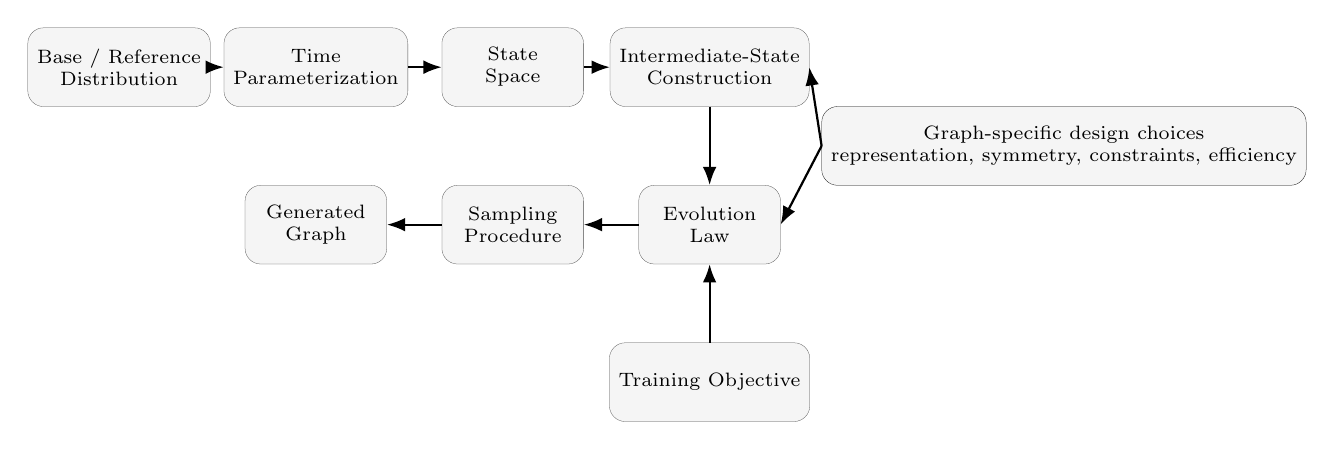
\begin{tikzpicture}[
    >=Latex,
    font=\scriptsize,
    box/.style={
        draw=black!70,
        rounded corners=2mm,
        ultra thin,
        minimum width=1.8cm,
        minimum height=1.0cm,
        align=center,
        fill=gray!8
    },
    side/.style={
        draw=black!70,
        rounded corners=2mm,
         ultra thin,
        minimum width=2.1cm,
        minimum height=1.0cm,
        align=center,
       fill=gray!8
    },
    note/.style={
        draw=black!70!black,
        rounded corners=2mm,
        ultra thin,
        minimum width=2.4cm,
        minimum height=1.0cm,
        align=center,
        fill=gray!8
    },
    annobox/.style={
        rounded corners=1.5mm,
        thin,
        inner sep=2pt,
        font=\scriptsize,
        align=center
    },
    arr/.style={->, thick}
]

% main pipeline: first row
\node[box] (base) at (0,0) {Base / Reference\\Distribution};
\node[box] (time) at (2.5,0) {Time\\Parameterization};
\node[box] (state) at (5.0,0) {State\\Space};
\node[box] (path) at (7.5,0) {Intermediate-State\\Construction};

% main pipeline: second row (right to left order)
\node[box] (out) at (2.5,-2.0) {Generated\\Graph};
\node[box] (sample) at (5.0,-2.0) {Sampling\\Procedure};
\node[box] (evo) at (7.5,-2.0) {Evolution\\Law};

\draw[arr] (base) -- (time);
\draw[arr] (time) -- (state);
\draw[arr] (state) -- (path);
\draw[arr] (path.south) -- ++(0,-0.4) -| (evo.north);
\draw[arr] (evo) -- (sample);
\draw[arr] (sample) -- (out);

% side components
\node[side] (train) at (7.5,-4.0) {Training Objective};
\draw[arr] (train.north) -- (evo.south);

\node[note] (graphspec) at (12.0,-1.0) {Graph-specific design choices\\representation, symmetry, constraints, efficiency};
\draw[arr] (graphspec.west) -- (path.east);
\draw[arr] (graphspec.west) -- (evo.east);

\end{tikzpicture}
\caption{General component template of time-dependent graph generative models.}
\label{fig:general_template_tdgg}
\end{figure*}

\subsection{Comparative Taxonomy of Time-Dependent Graph Generation}
\label{sec:taxonomy}

Building on the general template above, we organize time-dependent graph generative models through a comparative taxonomy. The goal of this taxonomy is not to define disjoint families, but to provide a compact structural map of the design space. In the remainder of the survey, this taxonomy serves mainly as an \emph{organizational guide}: it helps us group and order methods in Secs.~\ref{sec:discrete_time}, \ref{sec:continuous_time}, and \ref{sec:comparative_taxonomy}. Figure~\ref{fig:taxonomy_tdgg} summarizes the main axes.

\begin{figure*}[t]
\centering
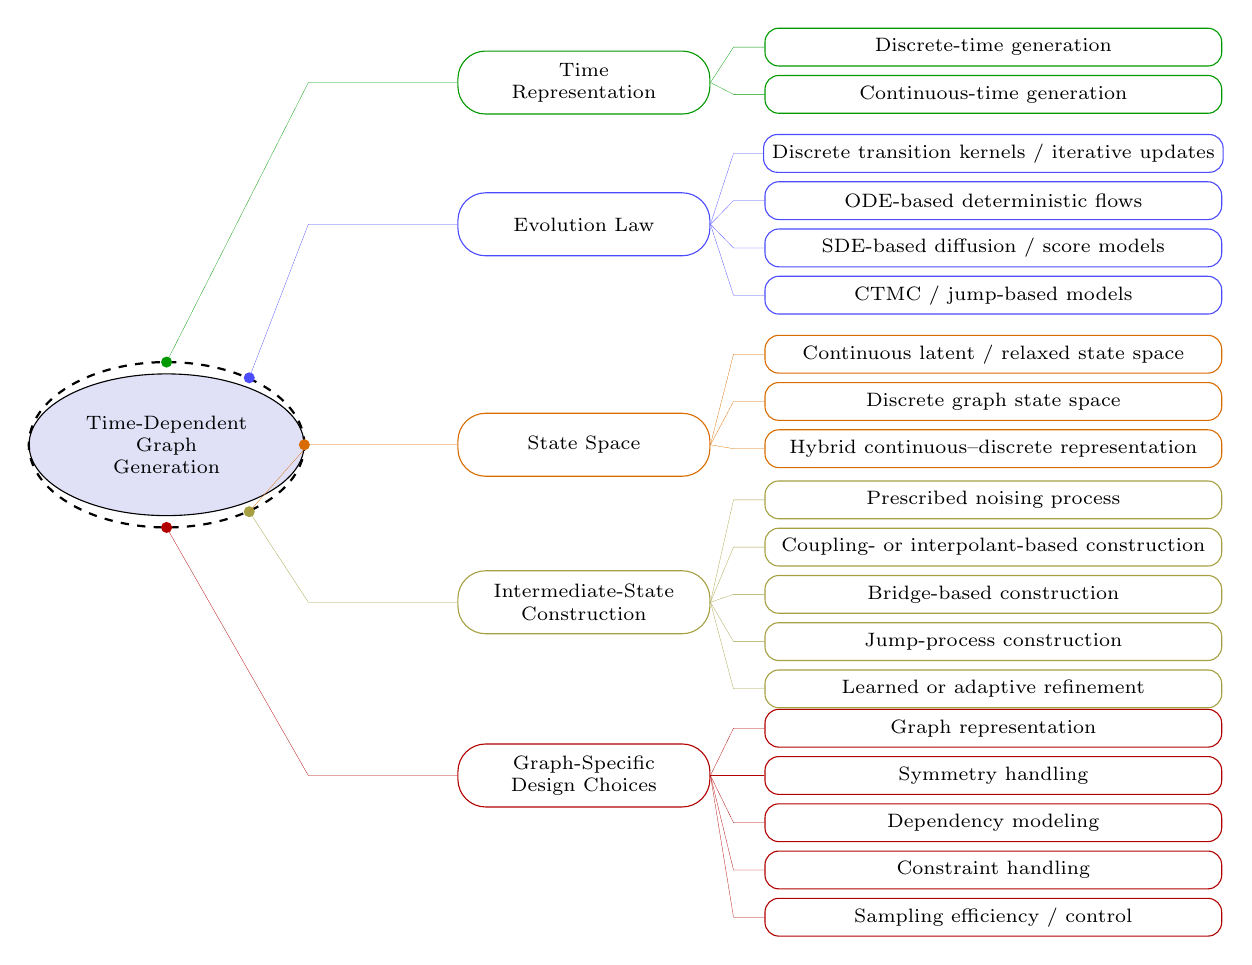
\begin{tikzpicture}[
    font=\scriptsize,
    line width=0.9pt,
    >=Latex,
    every node/.style={align=center},
    root/.style={
        ellipse,
        draw=black,
        thin,
        fill=blue!60!gray!15,
        minimum width=1.8cm,
        minimum height=1.8cm,
        inner sep=6pt
    },
    major/.style={
        rectangle,
        rounded corners=10pt,
        draw=#1,
        thin,
        fill=white,
        minimum width=3.2cm,
        minimum height=0.8cm,
        inner sep=3pt
    },
    leaf/.style={
        rectangle,
        rounded corners=5pt,
        draw=#1,
        thin,
        fill=white,
        minimum width=5.8cm,
        minimum height=0.48cm,
        inner sep=3pt
    },
]

\node[root] (root) at (0,0) {Time-Dependent\\Graph\\Generation};
\draw[dash pattern=on 3pt off 3pt, thick] (root) ellipse [x radius=1.75cm, y radius=1.05cm];

\fill[green!60!black]   (0.0, 1.05) circle (2pt);
\fill[blue!70]          (1.05, 0.85) circle (2pt);
\fill[orange!85!black]  (1.75,0.0) circle (2pt);
\fill[yellow!60!black]  (1.05,-0.85) circle (2pt);
\fill[red!70!black]     (0.0,-1.05) circle (2pt);

\node[major=green!60!black]  (time)  at (5.3,  4.6)  {Time\\Representation};
\node[major=blue!70]         (dyn)   at (5.3,  2.8)  {Evolution Law};
\node[major=orange!85!black] (state) at (5.3,  0.0)  {State Space};
\node[major=yellow!60!black] (inter) at (5.3, -2.0)  {Intermediate-State\\Construction};
\node[major=red!70!black]    (graph) at (5.3, -4.2)  {Graph-Specific\\Design Choices};

\draw[green!60!black, ultra thin] (0.0,1.05) -- (1.8,4.6) -- (time.west);
\draw[blue!70, ultra thin]         (1.05,0.85) -- (1.8,2.8) -- (dyn.west);
\draw[orange!85!black, ultra thin] (1.05,-0.85) -- (1.8,0.0) -- (state.west);
\draw[yellow!60!black, ultra thin] (1.05,-0.85) -- (1.8,-2.0) -- (inter.west);
\draw[red!70!black, ultra thin]    (0.0,-1.05) -- (1.8,-4.2) -- (graph.west);

\node[leaf=green!60!black] (time1) at (10.5, 5.05) {Discrete-time generation};
\node[leaf=green!60!black] (time2) at (10.5, 4.45) {Continuous-time generation};
\draw[green!60!black, ultra thin] (time.east) -- (7.2,5.05) -- (time1.west);
\draw[green!60!black, ultra thin] (time.east) -- (7.2,4.45) -- (time2.west);

\node[leaf=blue!70] (dyn1) at (10.5, 3.70) {Discrete transition kernels / iterative updates};
\node[leaf=blue!70] (dyn2) at (10.5, 3.10) {ODE-based deterministic flows};
\node[leaf=blue!70] (dyn3) at (10.5, 2.50) {SDE-based diffusion / score models};
\node[leaf=blue!70] (dyn4) at (10.5, 1.90) {CTMC / jump-based models};
\draw[blue!70, ultra thin] (dyn.east) -- (7.2,3.70) -- (dyn1.west);
\draw[blue!70, ultra thin] (dyn.east) -- (7.2,3.10) -- (dyn2.west);
\draw[blue!70, ultra thin] (dyn.east) -- (7.2,2.50) -- (dyn3.west);
\draw[blue!70, ultra thin] (dyn.east) -- (7.2,1.90) -- (dyn4.west);

\node[leaf=orange!85!black] (st1) at (10.5, 1.15) {Continuous latent / relaxed state space};
\node[leaf=orange!85!black] (st2) at (10.5, 0.55) {Discrete graph state space};
\node[leaf=orange!85!black] (st3) at (10.5, -0.05) {Hybrid continuous--discrete representation};
\draw[orange!85!black, ultra thin] (state.east) -- (7.2,1.15) -- (st1.west);
\draw[orange!85!black, ultra thin] (state.east) -- (7.2,0.55) -- (st2.west);
\draw[orange!85!black, ultra thin] (state.east) -- (7.2,-0.05) -- (st3.west);

\node[leaf=yellow!60!black] (i1) at (10.5, -0.70) {Prescribed noising process};
\node[leaf=yellow!60!black] (i2) at (10.5, -1.30) {Coupling- or interpolant-based construction};
\node[leaf=yellow!60!black] (i3) at (10.5, -1.90) {Bridge-based construction};
\node[leaf=yellow!60!black] (i4) at (10.5, -2.50) {Jump-process construction};
\node[leaf=yellow!60!black] (i5) at (10.5, -3.10) {Learned or adaptive refinement};
\draw[yellow!60!black, ultra thin] (inter.east) -- (7.2,-0.70) -- (i1.west);
\draw[yellow!60!black, ultra thin] (inter.east) -- (7.2,-1.30) -- (i2.west);
\draw[yellow!60!black, ultra thin] (inter.east) -- (7.2,-1.90) -- (i3.west);
\draw[yellow!60!black, ultra thin] (inter.east) -- (7.2,-2.50) -- (i4.west);
\draw[yellow!60!black, ultra thin] (inter.east) -- (7.2,-3.10) -- (i5.west);

\node[leaf=red!70!black] (g1) at (10.5, -3.60) {Graph representation};
\node[leaf=red!70!black] (g2) at (10.5, -4.20) {Symmetry handling};
\node[leaf=red!70!black] (g3) at (10.5, -4.80) {Dependency modeling};
\node[leaf=red!70!black] (g4) at (10.5, -5.40) {Constraint handling};
\node[leaf=red!70!black] (g5) at (10.5, -6.00) {Sampling efficiency / control};
\draw[red!70!black, ultra thin] (graph.east) -- (7.2,-3.60) -- (g1.west);
\draw[red!70!black, ultra thin] (graph.east) -- (7.2,-4.20) -- (g2.west);
\draw[red!70!black, ultra thin] (graph.east) -- (7.2,-4.80) -- (g3.west);
\draw[red!70!black, ultra thin] (graph.east) -- (7.2,-5.40) -- (g4.west);
\draw[red!70!black, ultra thin] (graph.east) -- (7.2,-6.00) -- (g5.west);

\end{tikzpicture}
\caption{A comparative taxonomy of time-dependent graph generative models.}
\label{fig:taxonomy_tdgg}
\end{figure*}

We use the following taxonomy axes to organize the method space:
\begin{itemize}[leftmargin=*]
    \item \textbf{Time representation:} whether generation is defined over discrete steps or continuous time.
    \item \textbf{Evolution law:} the local mechanism that drives the process, such as discrete transition kernels, iterative updates, ODE flows, reverse SDE dynamics, or CTMC jump rates.
    \item \textbf{State space:} whether the process evolves in discrete graph space, a continuous relaxation, a latent space, or a hybrid representation.
    \item \textbf{Intermediate-state construction:} how the path between source and target is defined, for example by prescribed noising, interpolation, bridge construction, jump dynamics, or learned refinement.
    \item \textbf{Graph-specific design choices:} how a general time-dependent generator is specialized to graph domains through representation design, symmetry handling, dependency modeling, constraint control, and sampling efficiency.
\end{itemize}

Taken together, these axes tell us how methods are built and where they sit in the design space. 

\subsection{A Challenge-Oriented Reading Guide}
\label{sec:challenge_reading_guide}

While the taxonomy above organizes methods by design, we also need a second lens for comparison: the recurring challenges of graph generation. In later sections, this challenge-oriented view provides the main criteria for evaluating representative methods. In this sense, the taxonomy tells us \emph{how to organize the models}, whereas the challenge-oriented guide tells us \emph{how to assess them}.

We focus on six recurring challenges \cite{guo2022systematic}:
\begin{itemize}[leftmargin=*]
    \item \textbf{Non-unique representations:} the same graph can admit many equivalent representations under node permutations or different construction orders.
    \item \textbf{Complex dependencies:} nodes and edges are not independent and often exhibit higher-order structural correlations.
    \item \textbf{Large output spaces:} the number of possible graphs grows combinatorially with graph size, making search and sampling difficult.
    \item \textbf{Evaluation for implicit properties:} many important graph characteristics are global or indirect and are not fully captured by simple local statistics.
    \item \textbf{Various validity requirements:} different application domains impose different structural constraints, such as chemical validity, connectivity, acyclicity, or type consistency.
    \item \textbf{Black-box behavior with low reliability:} many deep graph generators remain difficult to interpret, diagnose, or control.
\end{itemize}

\paragraph{Qualitative assessment scale.}
In later sections, we summarize how directly a method addresses each challenge using a coarse qualitative scale:
\emph{Strong}, \emph{Moderate}, and \emph{Weak}. Here, \emph{Strong} means that the challenge is explicitly handled by the model design, \emph{Moderate} means that it is only partially or indirectly addressed, and \emph{Weak} means that it is largely left unresolved or handled only through post hoc effects.

These challenges are not additional taxonomy axes. Rather, they form an evaluative layer on top of the taxonomy. Accordingly, in Secs.~\ref{sec:discrete_time} and \ref{sec:continuous_time}, we discuss each model both in terms of where it belongs in the design space and in terms of how well its design addresses these recurring challenges.












\section{Discrete-Time Graph Generation}
\label{sec:discrete_time}

Figure~\ref{fig:generic_discrete_time_architecture} summarizes the common template underlying discrete-time graph generation methods. The top row depicts a \emph{forward discrete-time process} that transforms an observed initial state $z_0$ into progressively modified intermediate states $z_t$ and finally into a terminal state $z_T$ through a finite number of steps. Depending on the method family, this forward mechanism may correspond to corruption, masking, editing, or partial construction. The bottom row shows the corresponding \emph{learned reverse process}, which starts from a simple initial state $z_T$ and iteratively refines it through intermediate states $z_t$ until reaching the final generated state $z_0$. The central learned component is a time-conditioned transition model $\phi_\theta(z_t,t)$ that predicts the next reverse update at each step. In this way, the figure highlights the key shared structure of discrete-time methods: a finite horizon, explicit intermediate states, and a stepwise reverse transition rule. It also shows that the same generic template can cover several subfamilies, including denoising and diffusion models, absorbing or masking models, autoregressive or sequential constructions, and editing or refinement-based generators.


\begin{figure*}[http]
\centering
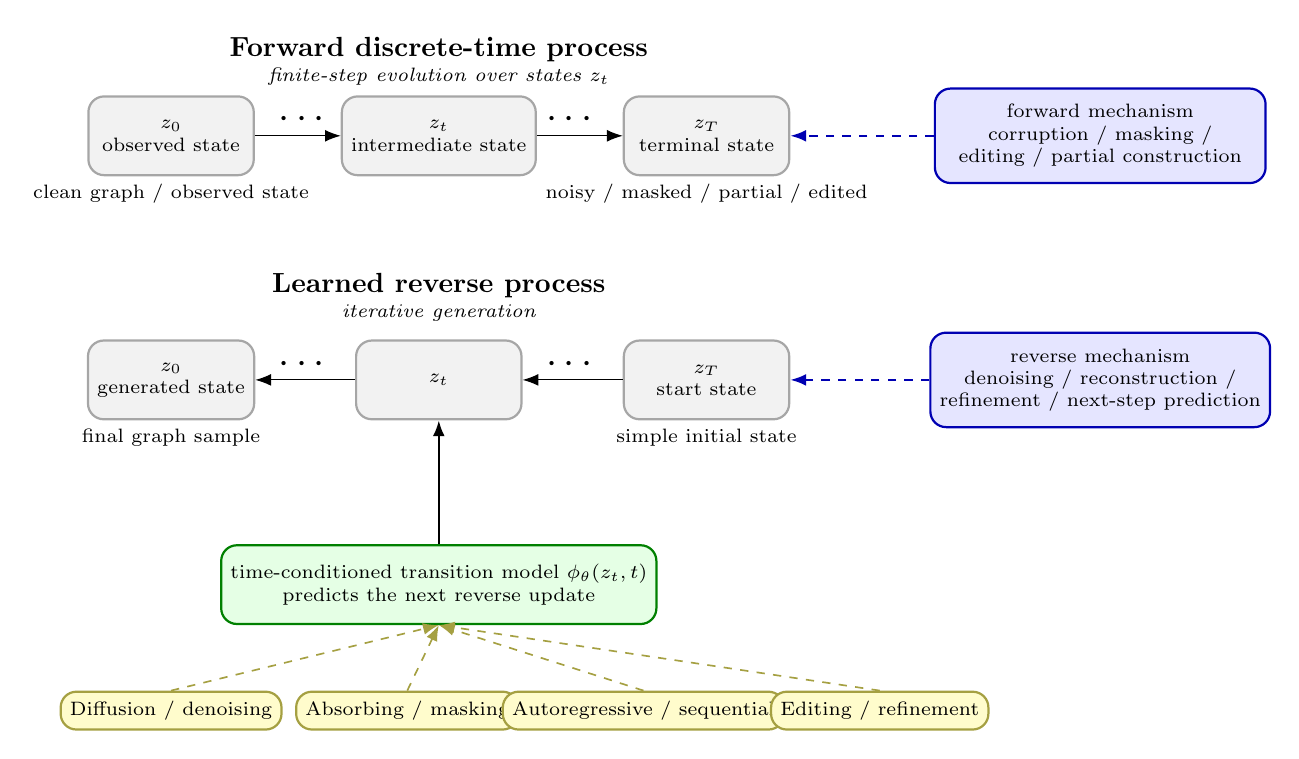
\begin{tikzpicture}[
    >=Latex,
    font=\sffamily,
    state/.style={
        draw=gray!70,
        rounded corners=2mm,
        thick,
        minimum width=2.1cm,
        minimum height=1.0cm,
        align=center,
        fill=gray!10,
        font=\scriptsize
    },
    sidebox/.style={
        draw=blue!70!black,
        rounded corners=2mm,
        thick,
        minimum width=4.2cm,
        minimum height=1.2cm,
        align=center,
        fill=blue!10,
        font=\scriptsize
    },
    greenbox/.style={
        font=\scriptsize,
        draw=green!50!black,
        rounded corners=2mm,
        thick,
        minimum width=2.3cm,
        minimum height=1.0cm,
        align=center,
        fill=green!10
    },
    note/.style={
        draw=yellow!60!black,
        rounded corners=2mm,
        thick,
        font=\scriptsize,
        minimum width=1.3cm,
        minimum height=0.4cm,
        align=center,
        fill=yellow!20
    },
    annobox/.style={
        rounded corners=1.5mm,
        thin,
        inner sep=2pt,
        font=\scriptsize,
        align=center
    },
    fwd/.style={thin, -{Latex[length=2mm]}},
    rev/.style={thin, -{Latex[length=2mm]}},
    aux/.style={blue!70!black, dashed, thick, -{Latex[length=2mm]}},
    goldaux/.style={
        yellow!60!black,
        font=\scriptsize,
        dashed,
        semithick,
        -{Latex[length=2mm]}
    },
    blackaux/.style={
        black,
        font=\scriptsize,
        thick,
        -{Latex[length=2mm]}
    }
]

% headings
\node[font=\bfseries] at (5.2,7.9) {Forward discrete-time process};
\node[font=\scriptsize\itshape] at (5.2,7.55) {finite-step evolution over states $z_t$};

\node[font=\bfseries] at (5.2,4.9) {Learned reverse process};
\node[font=\scriptsize\itshape] at (5.2,4.55) {iterative generation};

% top row
\node[state] (z0) at (1.8,6.8) {$z_0$\\observed state};
\node[annobox] at ($(z0.north)+(0,-1.25)$) {clean graph / observed state};

\node[state] (zt) at (5.2,6.8) {$z_t$\\intermediate state};

\node[state] (zT) at (8.6,6.8) {$z_T$\\terminal state};
\node[annobox] at ($(zT.north)+(0,-1.25)$) {noisy / masked / partial / edited};

\node[sidebox] (fbox) at (13.6,6.8)
{forward mechanism\\corruption / masking /\\editing / partial construction};

\draw[fwd] (z0.east) -- (zt.west);
\draw[fwd] (zt.east) -- (zT.west);
\draw[aux] (fbox.west) -- (zT.east);

\node[font=\Large] at (3.5,7.0) {$\cdots$};
\node[font=\Large] at (6.9,7.0) {$\cdots$};

% bottom row
\node[state] (rz0) at (1.8,3.7) {$z_0$\\generated state};
\node[annobox] at ($(rz0.north)+(0,-1.25)$) {final graph sample};

\node[state] (rzt) at (5.2,3.7) {$z_t$};

\node[state] (rzT) at (8.6,3.7) {$z_T$\\start state};
\node[annobox] at ($(rzT.north)+(0,-1.25)$) {simple initial state};

\node[sidebox] (rbox) at (13.6,3.7)
{reverse mechanism\\denoising / reconstruction /\\refinement / next-step prediction};

\draw[rev] (rzT.west) -- (rzt.east);
\draw[rev] (rzt.west) -- (rz0.east);
\draw[aux] (rbox.west) -- (rzT.east);

\node[font=\Large] at (3.5,3.9) {$\cdots$};
\node[font=\Large] at (6.9,3.9) {$\cdots$};

% model box
\node[greenbox] (phi) at (5.2,1.1)
{time-conditioned transition model $\phi_\theta(z_t,t)$\\predicts the next reverse update};

\draw[blackaux] (phi.north) -- (rzt.south);

% notes
\node[note] (n1) at (1.8,-0.5) {Diffusion / denoising};
\node[note] (n2) at (4.8,-0.5) {Absorbing / masking};
\node[note] (n3) at (7.8,-0.5) {Autoregressive / sequential};
\node[note] (n4) at (10.8,-0.5) {Editing / refinement};

\draw[goldaux] (n1.north) -- (phi.south);
\draw[goldaux] (n2.north) -- (phi.south);
\draw[goldaux] (n3.north) -- (phi.south);
\draw[goldaux] (n4.north) -- (phi.south);

\end{tikzpicture}
\caption{Generic architecture of discrete-time graph generation.}
\label{fig:generic_discrete_time_architecture}
\end{figure*}


\subsection{Discrete-Time Denoising and Diffusion Models}
\label{sec:discrete_denoising_diffusion}

Discrete-time denoising and diffusion models form one of the central families of graph generation methods. They instantiate the generic finite-step template introduced above by defining a prescribed forward process that gradually corrupts, masks, or transforms a graph across a sequence of intermediate states, together with a learned reverse process that reconstructs the graph step by step. Their common appeal is that they provide an explicit trajectory over time-indexed states while retaining considerable flexibility in the choice of corruption kernel, state space, terminal reference distribution, and graph-specific constraints.

\begin{table}[H]
\centering
\footnotesize
\renewcommand{\arraystretch}{1.12}
\setlength{\tabcolsep}{3pt}
\begin{tabularx}{\columnwidth}{@{}>{\raggedright\arraybackslash}p{2.0cm}
                                >{\raggedright\arraybackslash}p{3.0cm}
                                >{\raggedright\arraybackslash}p{2.0cm}
                                X@{}}
\toprule
\textbf{Model} & \textbf{Space} & \textbf{Path} & \textbf{Key idea} \\
\midrule
GraphGUIDE & discrete & Bernoulli & interpretable editing \\
EDP        & discrete & Markov & efficient discrete diffusion \\
DiGress    & discrete/attributed & categorical & joint node--edge denoising \\
ConStruct  & discrete/constrained & absorbing & validity preservation \\
EDGE       & discrete/sparse & edge-removal & scalable sparse generation \\
GBD        & transformed/bounded & beta & bounded topology/attributes \\
GGSD       & transformed/spectral & Gaussian & spectral global structure \\
GraphARM   & hybrid/discrete & absorbing & autoregressive reverse order \\
LayerDAG   & DAG & hybrid & layerwise DAG generation \\
\bottomrule
\end{tabularx}
\caption{Representative discrete-time denoising and diffusion models.}
\label{tab:discrete_diffusion_keyword}
\end{table}

Within this family, the main design differences concern \emph{where} diffusion is performed and \emph{how} the reverse process is structured. Some methods remain entirely in discrete graph space and denoise node and edge variables directly. Others perform diffusion in transformed or alternative graph representations, such as bounded continuous variables or spectral spaces. A third line combines denoising-style refinement with absorbing transitions or autoregressive generation orderings. Table~\ref{tab:discrete_diffusion_keyword} summarizes representative models and their key design ideas.




In the discussion below, we organize these models into three subgroups: diffusion in discrete graph space, diffusion in transformed graph representations, and hybrid absorbing or autoregressive variants. This organization avoids treating discrete-time denoising as a single monolithic design and instead highlights the different ways in which finite-step corruption and reverse reconstruction can be adapted to graph structure.

\subsubsection{Diffusion in discrete graph space}
\label{sec:direct_discrete_diffusion}



The most direct branch of discrete-time denoising models operates on adjacency variables and, in the clearest cases, remains entirely in discrete graph space, so that each intermediate state is itself a graph rather than a continuous relaxation. This makes the trajectory easy to interpret in graph domain for example, through edge flips, deletions, or categorical relabeling---and provides a natural interface for imposing structural rules during sampling. Models within this branch can nevertheless differ substantially in whether their intermediate states remain discrete or pass through continuous noisy adjacencies.



\paragraph{Binary edge-space denoising.}
\emph{GraphGUIDE}~\cite{tseng2023graphguide} defines a finite-horizon Bernoulli corruption chain directly in discrete edge space and learns a reverse process that reconstructs clean graphs from corrupted ones. Its main appeal is that intermediate states remain well-defined combinatorial graphs, which supports interpretability, controllability, and the enforcement of explicit structural constraints through edge-level editing. By contrast, \emph{EDP-GNN}~\cite{niu2020permutation} adopts score-based generative modeling with Gaussian perturbations on adjacency matrices, learns a permutation-equivariant score network, and samples through annealed Langevin dynamics before discretizing the final adjacency matrix. Its main appeal is permutation-invariant density modeling and structured edge prediction, rather than maintaining discrete graph intermediates throughout the trajectory. Figure~\ref{fig:graphguide_edpgnn_pipelines} compares two representative early examples,

\emph{Evaluation.} GraphGUIDE stands out for interpretability, controllability, and explicit structural control through discrete edge editing, but it does not fundamentally resolve permutation ambiguity, combinatorial graph-space growth, or the evaluation and control of higher-level implicit properties. EDP-GNN, while stronger on permutation ambiguity and structured edge dependencies, operates through continuous noisy adjacency states during sampling and does not explicitly enforce many domain-specific validity constraints.



% in preamble
% \usepackage{caption}
% \usepackage{subcaption}

\begin{figure*}[htbp]

\centering

\begin{subfigure}[t]{0.95\textwidth}
\centering
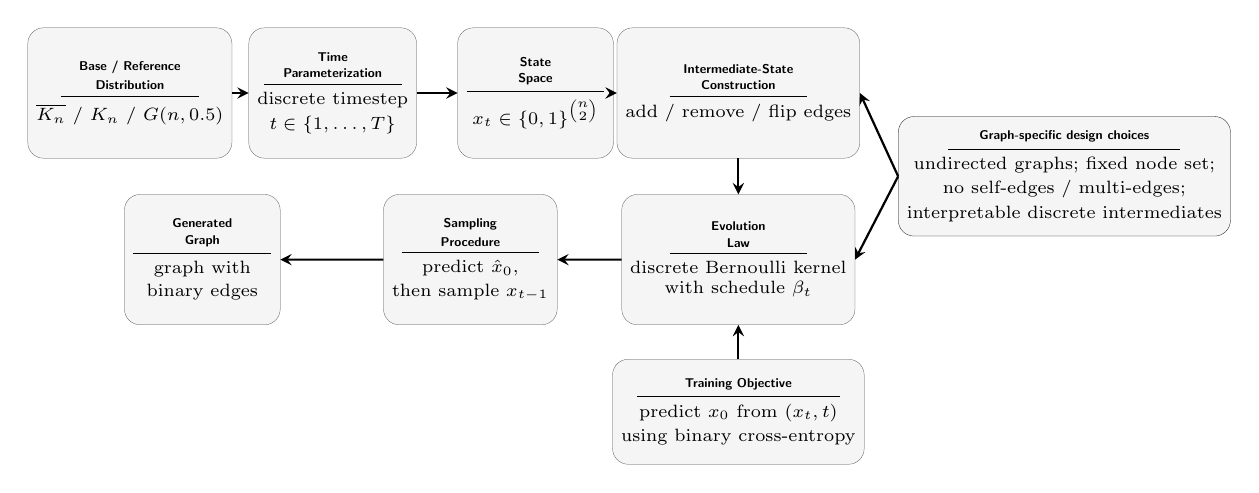
\begin{tikzpicture}[
    >=stealth,
    font=\scriptsize,
    scale=0.92,
    transform shape,
    box/.style={
        draw=black!70,
        rounded corners=2mm,
        ultra thin,
        minimum width=2.15cm,
        minimum height=1.8cm,
        align=center,
        fill=gray!8
    },
    side/.style={
        draw=black!70,
        rounded corners=2mm,
        ultra thin,
        minimum width=3.3cm,
        minimum height=1.45cm,
        align=center,
        fill=gray!8
    },
    note/.style={
        draw=black!70!black,
        rounded corners=2mm,
        ultra thin,
        minimum width=3.8cm,
        minimum height=1.65cm,
        align=center,
        fill=gray!8
    },
    arr/.style={->, thick}
]

% main pipeline: first row
\node[box] (base) at (0,0)
{\shortstack[c]{%
{\sffamily\bfseries\tiny Base / Reference}\\
{\sffamily\bfseries\tiny Distribution}\\[-0.2mm]
\rule{1.9cm}{0.2pt}\\[0.0mm]
$\overline{K_n}$ / $K_n$ / $G(n,0.5)$}};

\node[box] (time) at (2.8,0)
{\shortstack[c]{%
{\sffamily\bfseries\tiny Time}\\
{\sffamily\bfseries\tiny Parameterization}\\[-0.2mm]
\rule{1.9cm}{0.2pt}\\[0.0mm]
discrete timestep\\
$t \in \{1,\ldots,T\}$}};

\node[box] (state) at (5.6,0)
{\shortstack[c]{%
{\sffamily\bfseries\tiny State}\\
{\sffamily\bfseries\tiny Space}\\[-0.2mm]
\rule{1.9cm}{0.2pt}\\[0.0mm]
$x_t \in \{0,1\}^{\binom{n}{2}}$}};

\node[box] (path) at (8.4,0)
{\shortstack[c]{%
{\sffamily\bfseries\tiny Intermediate-State}\\
{\sffamily\bfseries\tiny Construction}\\[-0.2mm]
\rule{1.9cm}{0.2pt}\\[0.0mm]
add / remove / flip edges}};

% second row
\node[box] (out) at (1.0,-2.3)
{\shortstack[c]{%
{\sffamily\bfseries\tiny Generated}\\
{\sffamily\bfseries\tiny Graph}\\[-0.2mm]
\rule{1.9cm}{0.2pt}\\[0.0mm]
graph with\\
binary edges}};

\node[box] (sample) at (4.7,-2.3)
{\shortstack[c]{%
{\sffamily\bfseries\tiny Sampling}\\
{\sffamily\bfseries\tiny Procedure}\\[-0.2mm]
\rule{1.9cm}{0.2pt}\\[0.0mm]
predict $\hat{x}_0$,\\
then sample $x_{t-1}$}};

\node[box] (evo) at (8.4,-2.3)
{\shortstack[c]{%
{\sffamily\bfseries\tiny Evolution}\\
{\sffamily\bfseries\tiny Law}\\[-0.2mm]
\rule{1.9cm}{0.2pt}\\[0.0mm]
discrete Bernoulli kernel\\
with schedule $\beta_t$}};

\draw[arr] (base) -- (time);
\draw[arr] (time) -- (state);
\draw[arr] (state) -- (path);
\draw[arr] (path.south) -- ++(0,-0.45) -| (evo.north);
\draw[arr] (evo) -- (sample);
\draw[arr] (sample) -- (out);

% side components
\node[side] (train) at (8.4,-4.4)
{\shortstack[c]{%
{\sffamily\bfseries\tiny Training Objective}\\[-0.2mm]
\rule{2.8cm}{0.2pt}\\[0.0mm]
predict $x_0$ from $(x_t,t)$\\
using binary cross-entropy}};
\draw[arr] (train.north) -- (evo.south);

\node[note] (graphspec) at (12.9,-1.15)
{\shortstack[c]{%
{\sffamily\bfseries\tiny Graph-specific design choices}\\[-0.2mm]
\rule{3.2cm}{0.2pt}\\[0.0mm]
undirected graphs; fixed node set;\\
no self-edges / multi-edges;\\
interpretable discrete intermediates}};
\draw[arr] (graphspec.west) -- (path.east);
\draw[arr] (graphspec.west) -- (evo.east);

\end{tikzpicture}
\caption{GraphGUIDE.}
\label{fig:graphguide_pipeline}
\end{subfigure}

\vspace{0.8em}

\begin{subfigure}[t]{0.95\textwidth}
\centering
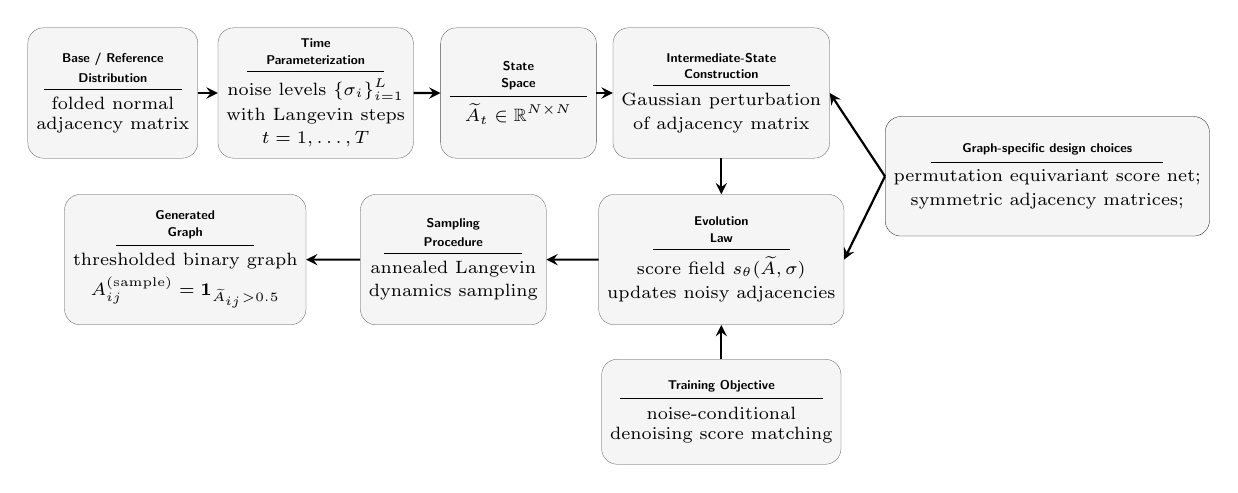
\begin{tikzpicture}[
    >=stealth,
    font=\scriptsize,
    scale=0.92,
    transform shape,
    box/.style={
        draw=black!70,
        rounded corners=2mm,
        ultra thin,
        minimum width=2.15cm,
        minimum height=1.8cm,
        align=center,
        fill=gray!8
    },
    side/.style={
        draw=black!70,
        rounded corners=2mm,
        ultra thin,
        minimum width=3.3cm,
        minimum height=1.45cm,
        align=center,
        fill=gray!8
    },
    note/.style={
        draw=black!70!black,
        rounded corners=2mm,
        ultra thin,
        minimum width=3.8cm,
        minimum height=1.65cm,
        align=center,
        fill=gray!8
    },
    arr/.style={->, thick}
]

% main pipeline: first row
\node[box] (base) at (0,0)
{\shortstack[c]{%
{\sffamily\bfseries\tiny Base / Reference}\\
{\sffamily\bfseries\tiny Distribution}\\[-0.2mm]
\rule{1.9cm}{0.2pt}\\[0.0mm]
folded normal\\
adjacency matrix}};

\node[box] (time) at (2.8,0)
{\shortstack[c]{%
{\sffamily\bfseries\tiny Time}\\
{\sffamily\bfseries\tiny Parameterization}\\[-0.2mm]
\rule{1.9cm}{0.2pt}\\[0.0mm]
noise levels $\{\sigma_i\}_{i=1}^L$\\
with Langevin steps\\ $t=1,\dots,T$}};

\node[box] (state) at (5.6,0)
{\shortstack[c]{%
{\sffamily\bfseries\tiny State}\\
{\sffamily\bfseries\tiny Space}\\[-0.2mm]
\rule{1.9cm}{0.2pt}\\[0.0mm]
$\widetilde{A}_t \in \mathbb{R}^{N\times N}$}};

\node[box] (path) at (8.4,0)
{\shortstack[c]{%
{\sffamily\bfseries\tiny Intermediate-State}\\
{\sffamily\bfseries\tiny Construction}\\[-0.2mm]
\rule{1.9cm}{0.2pt}\\[0.0mm]
Gaussian perturbation\\
of adjacency matrix}};

% second row
\node[box] (out) at (1.0,-2.3)
{\shortstack[c]{%
{\sffamily\bfseries\tiny Generated}\\
{\sffamily\bfseries\tiny Graph}\\[-0.2mm]
\rule{1.9cm}{0.2pt}\\[0.0mm]
thresholded binary graph\\
$A^{(\mathrm{sample})}_{ij}=\mathbf{1}_{\widetilde{A}_{ij}>0.5}$}};

\node[box] (sample) at (4.7,-2.3)
{\shortstack[c]{%
{\sffamily\bfseries\tiny Sampling}\\
{\sffamily\bfseries\tiny Procedure}\\[-0.2mm]
\rule{1.9cm}{0.2pt}\\[0.0mm]
annealed Langevin\\
dynamics sampling}};

\node[box] (evo) at (8.4,-2.3)
{\shortstack[c]{%
{\sffamily\bfseries\tiny Evolution}\\
{\sffamily\bfseries\tiny Law}\\[-0.2mm]
\rule{1.9cm}{0.2pt}\\[0.0mm]
score field $s_\theta(\widetilde{A},\sigma)$\\
updates noisy adjacencies}};

\draw[arr] (base) -- (time);
\draw[arr] (time) -- (state);
\draw[arr] (state) -- (path);
\draw[arr] (path.south) -- ++(0,-0.45) -| (evo.north);
\draw[arr] (evo) -- (sample);
\draw[arr] (sample) -- (out);

% side components
\node[side] (train) at (8.4,-4.4)
{\shortstack[c]{%
{\sffamily\bfseries\tiny Training Objective}\\[-0.2mm]
\rule{2.8cm}{0.2pt}\\[0.0mm]
noise-conditional\\
denoising score matching}};
\draw[arr] (train.north) -- (evo.south);

\node[note] (graphspec) at (12.9,-1.15)
{\shortstack[c]{%
{\sffamily\bfseries\tiny Graph-specific design choices}\\[-0.2mm]
\rule{3.2cm}{0.2pt}\\[0.0mm]
permutation equivariant score net;\\
symmetric adjacency matrices;}};
\draw[arr] (graphspec.west) -- (path.east);
\draw[arr] (graphspec.west) -- (evo.east);

\end{tikzpicture}
\caption{EDP-GNN.}
\label{fig:edpgnn_pipeline}
\end{subfigure}

\caption{Comparison of two time-dependent graph generation pipelines: (a) GraphGUIDE, which operates in discrete edge space with Bernoulli transitions, and (b) EDP-GNN, which operates in continuous symmetric adjacency space with score-based sampling.}
\label{fig:graphguide_edpgnn_pipelines}
\end{figure*}


\paragraph{Categorical node--edge diffusion.}

\emph{DiGress}~\cite{vignac2022digress} extends discrete denoising from binary edge existence to \emph{attributed discrete graphs} by diffusing both node types and edge types with categorical Markov transitions, treating edge absence as a special edge category. This keeps the entire trajectory discrete while allowing a single framework for both molecular and non-molecular attributed graphs. Relative to GraphGUIDE and EDP-GNN, the main difference is therefore not the overall finite-step denoising template, but the richer discrete state space and the corresponding reverse problem, which becomes a joint node--edge classification task. Figure~\ref{fig:digress_pipeline} summarizes the DiGress pipeline. 

\emph{Evaluation.} DiGress is particularly strong at preserving discrete graph structure throughout sampling, handling permutation ambiguity through a permutation-equivariant graph transformer, and modeling dependencies among categorical node and edge attributes. However, it remains computationally demanding on larger graphs, many important graph properties are still evaluated only indirectly, and domain-specific validity is not enforced by construction.


\begin{figure*}[htbp]
\captionsetup{font=footnotesize}
\captionsetup[subfigure]{font=footnotesize}
\centering

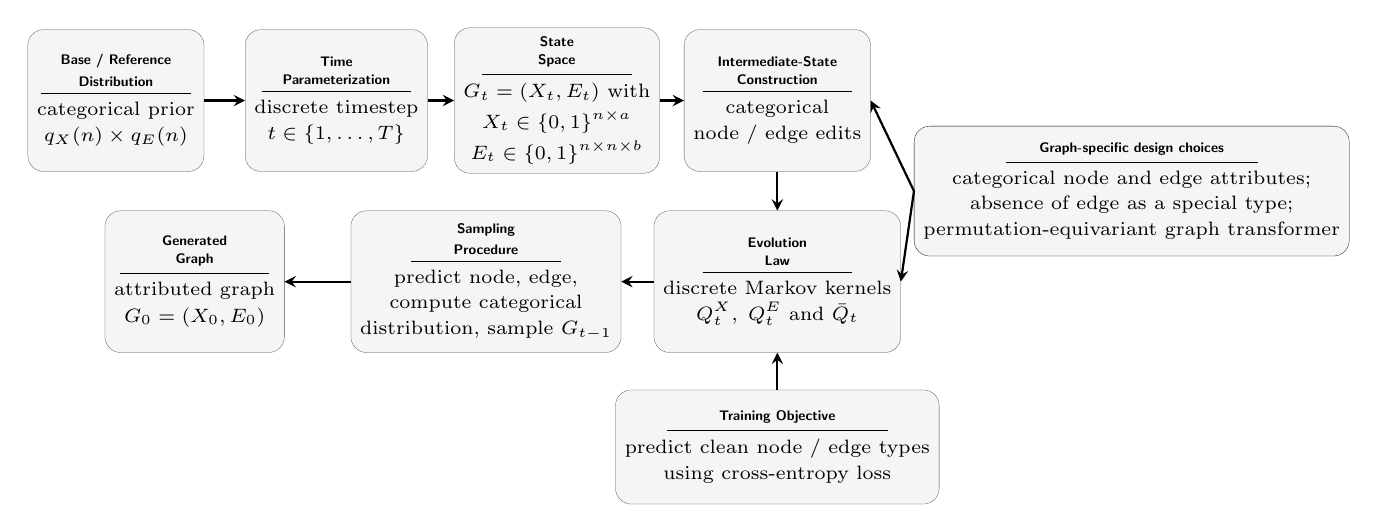
\begin{tikzpicture}[
    >=stealth,
    font=\scriptsize,
    box/.style={
        draw=black!70,
        rounded corners=2mm,
        ultra thin,
        minimum width=2.15cm,
        minimum height=1.8cm,
        align=center,
        fill=gray!8
    },
    side/.style={
        draw=black!70,
        rounded corners=2mm,
        ultra thin,
        minimum width=3.3cm,
        minimum height=1.45cm,
        align=center,
        fill=gray!8
    },
    note/.style={
        draw=black!70!black,
        rounded corners=2mm,
        ultra thin,
        minimum width=3.8cm,
        minimum height=1.65cm,
        align=center,
        fill=gray!8
    },
    arr/.style={->, thick}
]

% main pipeline: first row
\node[box] (base) at (0,0)
{\shortstack[c]{%
{\sffamily\bfseries\tiny Base / Reference}\\
{\sffamily\bfseries\tiny Distribution}\\[-0.2mm]
\rule{1.9cm}{0.2pt}\\[0.0mm]
categorical prior\\
$q_X(n)\times q_E(n)$}};

\node[box] (time) at (2.8,0)
{\shortstack[c]{%
{\sffamily\bfseries\tiny Time}\\
{\sffamily\bfseries\tiny Parameterization}\\[-0.2mm]
\rule{1.9cm}{0.2pt}\\[0.0mm]
discrete timestep\\
$t \in \{1,\ldots,T\}$}};

\node[box] (state) at (5.6,0)
{\shortstack[c]{%
{\sffamily\bfseries\tiny State}\\
{\sffamily\bfseries\tiny Space}\\[-0.2mm]
\rule{1.9cm}{0.2pt}\\[0.0mm]
$G_t=(X_t,E_t)$ with\\
$X_t\in\{0,1\}^{n\times a}$ \\
$E_t\in\{0,1\}^{n\times n\times b}$}};

\node[box] (path) at (8.4,0)
{\shortstack[c]{%
{\sffamily\bfseries\tiny Intermediate-State}\\
{\sffamily\bfseries\tiny Construction}\\[-0.2mm]
\rule{1.9cm}{0.2pt}\\[0.0mm]
categorical \\ node / edge edits}};

% second row
\node[box] (out) at (1.0,-2.3)
{\shortstack[c]{%
{\sffamily\bfseries\tiny Generated}\\
{\sffamily\bfseries\tiny Graph}\\[-0.2mm]
\rule{1.9cm}{0.2pt}\\[0.0mm]
attributed graph\\
$G_0=(X_0,E_0)$}};

\node[box] (sample) at (4.7,-2.3)
{\shortstack[c]{%
{\sffamily\bfseries\tiny Sampling}\\
{\sffamily\bfseries\tiny Procedure}\\[-0.2mm]
\rule{1.9cm}{0.2pt}\\[0.0mm]
predict node, edge,\\
compute categorical \\distribution, sample $G_{t-1}$}};

\node[box] (evo) at (8.4,-2.3)
{\shortstack[c]{%
{\sffamily\bfseries\tiny Evolution}\\
{\sffamily\bfseries\tiny Law}\\[-0.2mm]
\rule{1.9cm}{0.2pt}\\[0.0mm]
discrete Markov kernels\\
$Q_t^X,\;Q_t^E$ and $\bar Q_t$}};

\draw[arr] (base) -- (time);
\draw[arr] (time) -- (state);
\draw[arr] (state) -- (path);
\draw[arr] (path.south) -- ++(0,-0.45) -| (evo.north);
\draw[arr] (evo) -- (sample);
\draw[arr] (sample) -- (out);

% side components
\node[side] (train) at (8.4,-4.4)
{\shortstack[c]{%
{\sffamily\bfseries\tiny Training Objective}\\[-0.2mm]
\rule{2.8cm}{0.2pt}\\[0.0mm]
predict clean node / edge types\\
using cross-entropy loss}};

\draw[arr] (train.north) -- (evo.south);

\node[note] (graphspec) at (12.9,-1.15)
{\shortstack[c]{%
{\sffamily\bfseries\tiny Graph-specific design choices}\\[-0.2mm]
\rule{3.2cm}{0.2pt}\\[0.0mm]
categorical node and edge attributes;\\
absence of edge as a special type;\\
permutation-equivariant graph transformer}};

\draw[arr] (graphspec.west) -- (path.east);
\draw[arr] (graphspec.west) -- (evo.east);

\end{tikzpicture}
\caption{DiGress pipeline. The model applies discrete diffusion to categorical node and edge types using Markov transition matrices,}
\label{fig:digress_pipeline}
\end{figure*}

\paragraph{Constraint-aware and sparse variants.}
\emph{ConStruct}~\cite{madeira2024generative} and \emph{EDGE}~\cite{chen2023efficient} illustrate two important extensions of direct discrete diffusion. ConStruct modifies both the forward and reverse procedures to preserve hard structural properties, combining edge-absorbing corruption with a projector that removes invalid reverse proposals. EDGE, by contrast, targets large sparse graphs and redesigns the reverse process around an empty-graph prior, active-node factorization, and degree guidance. In both cases, the core discrete-time denoising template is retained, but the reverse chain is explicitly structured to enforce validity, exploit sparsity, or control graph statistics.


% in preamble
% \usepackage{caption}
% \usepackage{subcaption}

\begin{figure*}[htbp]

\centering

\begin{subfigure}[t]{0.95\textwidth}
\centering
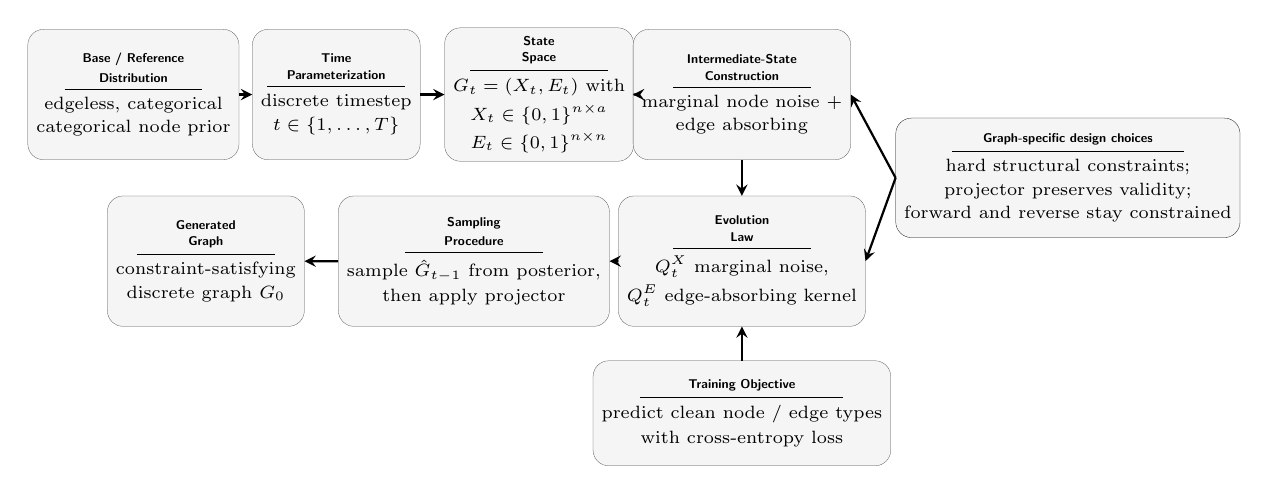
\begin{tikzpicture}[
    >=stealth,
    font=\scriptsize,
    scale=0.92,
    transform shape,
    box/.style={
        draw=black!70,
        rounded corners=2mm,
        ultra thin,
        minimum width=2.15cm,
        minimum height=1.8cm,
        align=center,
        fill=gray!8
    },
    side/.style={
        draw=black!70,
        rounded corners=2mm,
        ultra thin,
        minimum width=3.3cm,
        minimum height=1.45cm,
        align=center,
        fill=gray!8
    },
    note/.style={
        draw=black!70!black,
        rounded corners=2mm,
        ultra thin,
        minimum width=3.8cm,
        minimum height=1.65cm,
        align=center,
        fill=gray!8
    },
    arr/.style={->, thick}
]

% ConStruct: first row
\node[box] (base) at (0,0)
{\shortstack[c]{%
{\sffamily\bfseries\tiny Base / Reference}\\
{\sffamily\bfseries\tiny Distribution}\\[-0.2mm]
\rule{1.9cm}{0.2pt}\\[0.0mm]
edgeless, categorical\\
categorical node prior}};

\node[box] (time) at (2.8,0)
{\shortstack[c]{%
{\sffamily\bfseries\tiny Time}\\
{\sffamily\bfseries\tiny Parameterization}\\[-0.2mm]
\rule{1.9cm}{0.2pt}\\[0.0mm]
discrete timestep\\
$t \in \{1,\ldots,T\}$}};

\node[box] (state) at (5.6,0)
{\shortstack[c]{%
{\sffamily\bfseries\tiny State}\\
{\sffamily\bfseries\tiny Space}\\[-0.2mm]
\rule{1.9cm}{0.2pt}\\[0.0mm]
$G_t=(X_t,E_t)$ with\\
$X_t\in\{0,1\}^{n\times a}$ \\
$E_t\in\{0,1\}^{n\times n}$}};

\node[box] (path) at (8.4,0)
{\shortstack[c]{%
{\sffamily\bfseries\tiny Intermediate-State}\\
{\sffamily\bfseries\tiny Construction}\\[-0.2mm]
\rule{1.9cm}{0.2pt}\\[0.0mm]
marginal node noise +\\
edge absorbing}};

% ConStruct: second row
\node[box] (out) at (1.0,-2.3)
{\shortstack[c]{%
{\sffamily\bfseries\tiny Generated}\\
{\sffamily\bfseries\tiny Graph}\\[-0.2mm]
\rule{1.9cm}{0.2pt}\\[0.0mm]
constraint-satisfying\\
discrete graph $G_0$}};

\node[box] (sample) at (4.7,-2.3)
{\shortstack[c]{%
{\sffamily\bfseries\tiny Sampling}\\
{\sffamily\bfseries\tiny Procedure}\\[-0.2mm]
\rule{1.9cm}{0.2pt}\\[0.0mm]
sample $\hat G_{t-1}$ from posterior,\\
then apply projector}};

\node[box] (evo) at (8.4,-2.3)
{\shortstack[c]{%
{\sffamily\bfseries\tiny Evolution}\\
{\sffamily\bfseries\tiny Law}\\[-0.2mm]
\rule{1.9cm}{0.2pt}\\[0.0mm]
$Q_t^X$ marginal noise,\\
$Q_t^E$ edge-absorbing kernel}};

\draw[arr] (base) -- (time);
\draw[arr] (time) -- (state);
\draw[arr] (state) -- (path);
\draw[arr] (path.south) -- ++(0,-0.45) -| (evo.north);
\draw[arr] (evo) -- (sample);
\draw[arr] (sample) -- (out);

% side components
\node[side] (train) at (8.4,-4.4)
{\shortstack[c]{%
{\sffamily\bfseries\tiny Training Objective}\\[-0.2mm]
\rule{2.8cm}{0.2pt}\\[0.0mm]
predict clean node / edge types\\
with cross-entropy loss}};

\draw[arr] (train.north) -- (evo.south);

\node[note] (graphspec) at (12.9,-1.15)
{\shortstack[c]{%
{\sffamily\bfseries\tiny Graph-specific design choices}\\[-0.2mm]
\rule{3.2cm}{0.2pt}\\[0.0mm]
hard structural constraints;\\
projector preserves validity;\\
forward and reverse stay constrained}};

\draw[arr] (graphspec.west) -- (path.east);
\draw[arr] (graphspec.west) -- (evo.east);

\end{tikzpicture}
\caption{ConStruct.}
\label{fig:construct_pipeline}
\end{subfigure}

\vspace{0.8em}

\begin{subfigure}[t]{0.95\textwidth}
\centering
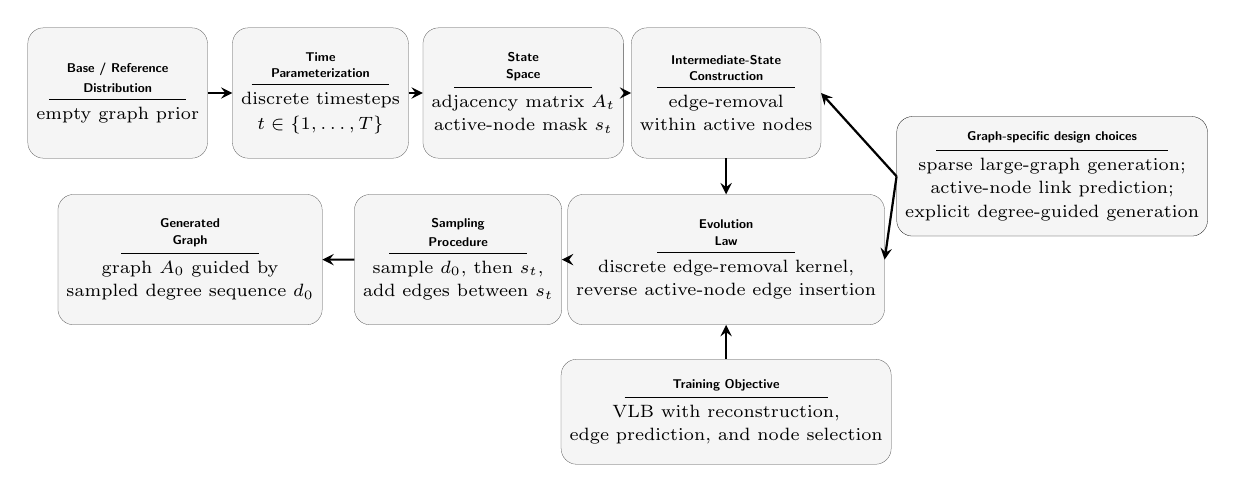
\begin{tikzpicture}[
    >=stealth,
    font=\scriptsize,
    scale=0.92,
    transform shape,
    box/.style={
        draw=black!70,
        rounded corners=2mm,
        ultra thin,
        minimum width=2.15cm,
        minimum height=1.8cm,
        align=center,
        fill=gray!8
    },
    side/.style={
        draw=black!70,
        rounded corners=2mm,
        ultra thin,
        minimum width=3.3cm,
        minimum height=1.45cm,
        align=center,
        fill=gray!8
    },
    note/.style={
        draw=black!70!black,
        rounded corners=2mm,
        ultra thin,
        minimum width=3.8cm,
        minimum height=1.65cm,
        align=center,
        fill=gray!8
    },
    arr/.style={->, thick}
]

% EDGE: first row
\node[box] (base) at (0,0)
{\shortstack[c]{%
{\sffamily\bfseries\tiny Base / Reference}\\
{\sffamily\bfseries\tiny Distribution}\\[-0.2mm]
\rule{1.9cm}{0.2pt}\\[0.0mm]
empty graph prior}};

\node[box] (time) at (2.8,0)
{\shortstack[c]{%
{\sffamily\bfseries\tiny Time}\\
{\sffamily\bfseries\tiny Parameterization}\\[-0.2mm]
\rule{1.9cm}{0.2pt}\\[0.0mm]
discrete timesteps\\
$t \in \{1,\ldots,T\}$}};

\node[box] (state) at (5.6,0)
{\shortstack[c]{%
{\sffamily\bfseries\tiny State}\\
{\sffamily\bfseries\tiny Space}\\[-0.2mm]
\rule{1.9cm}{0.2pt}\\[0.0mm]
adjacency matrix $A_t$\\
active-node mask $s_t$}};

\node[box] (path) at (8.4,0)
{\shortstack[c]{%
{\sffamily\bfseries\tiny Intermediate-State}\\
{\sffamily\bfseries\tiny Construction}\\[-0.2mm]
\rule{1.9cm}{0.2pt}\\[0.0mm]
edge-removal\\
within active nodes}};

% EDGE: second row
\node[box] (out) at (1.0,-2.3)
{\shortstack[c]{%
{\sffamily\bfseries\tiny Generated}\\
{\sffamily\bfseries\tiny Graph}\\[-0.2mm]
\rule{1.9cm}{0.2pt}\\[0.0mm]
graph $A_0$ guided by\\
sampled degree sequence $d_0$}};

\node[box] (sample) at (4.7,-2.3)
{\shortstack[c]{%
{\sffamily\bfseries\tiny Sampling}\\
{\sffamily\bfseries\tiny Procedure}\\[-0.2mm]
\rule{1.9cm}{0.2pt}\\[0.0mm]
sample $d_0$, then $s_t$,\\
add edges between $s_t$}};

\node[box] (evo) at (8.4,-2.3)
{\shortstack[c]{%
{\sffamily\bfseries\tiny Evolution}\\
{\sffamily\bfseries\tiny Law}\\[-0.2mm]
\rule{1.9cm}{0.2pt}\\[0.0mm]
discrete edge-removal kernel,\\
reverse active-node edge insertion}};

\draw[arr] (base) -- (time);
\draw[arr] (time) -- (state);
\draw[arr] (state) -- (path);
\draw[arr] (path.south) -- ++(0,-0.45) -| (evo.north);
\draw[arr] (evo) -- (sample);
\draw[arr] (sample) -- (out);

% side components
\node[side] (train) at (8.4,-4.4)
{\shortstack[c]{%
{\sffamily\bfseries\tiny Training Objective}\\[-0.2mm]
\rule{2.8cm}{0.2pt}\\[0.0mm]
VLB with reconstruction,\\
edge prediction, and node selection}};

\draw[arr] (train.north) -- (evo.south);

\node[note] (graphspec) at (12.9,-1.15)
{\shortstack[c]{%
{\sffamily\bfseries\tiny Graph-specific design choices}\\[-0.2mm]
\rule{3.2cm}{0.2pt}\\[0.0mm]
sparse large-graph generation;\\
active-node link prediction;\\
explicit degree-guided generation}};

\draw[arr] (graphspec.west) -- (path.east);
\draw[arr] (graphspec.west) -- (evo.east);

\end{tikzpicture}
\caption{EDGE.}
\label{fig:edge_pipeline}
\end{subfigure}

\caption{Comparison of two discrete-time graph generation pipelines: (a) ConStruct, which augments discrete graph diffusion with an edge-absorbing forward process and a projector to preserve structural constraints, and (b) EDGE, which uses an empty-graph convergent distribution, active-node reverse steps, and degree-guided generation for scalable large-graph synthesis.}
\label{fig:construct_edge_pipelines}
\end{figure*}


\emph{Evaluation.}
ConStruct and EDGE both preserve generation directly in discrete graph space through iterative denoising, but they prioritize different strengths. ConStruct is stronger in explicit structural control, since it enforces edge-deletion-invariant constraints throughout sampling via a constrained reverse process, whereas EDGE is stronger in scalability and statistical efficiency, using sparse active-node prediction and degree guidance to better handle large output spaces and degree-related structure. However, ConStruct still inherits the computational cost of dense discrete diffusion and depends on property-specific projector design, while EDGE does not fundamentally resolve permutation ambiguity, evaluates many implicit properties only through proxy statistics, and remains only partly interpretable despite its structured edge-removal and reconstruction mechanism.

Taken together, these models show that direct discrete graph-space diffusion is especially attractive when one wants interpretable intermediate graphs, explicit structural control, and reverse transitions that can be modified in graph-theoretic terms.

\subsubsection{Diffusion in transformed graph representations}
\label{sec:alternative_rep_discrete_diffusion}


A second branch retains the discrete-time denoising logic but changes the \emph{representation being diffused}. Instead of operating directly on discrete adjacency variables, these models evolve bounded  continuous graph variables or spectral graph representations. This choice often makes the forward and reverse transitions smoother or more expressive, but it also introduces an additional reconstruction gap between the representation trajectory and the final graph object.

\paragraph{Bounded continuous graph variables.}
\emph{GBD}~\cite{liu2024advancing} replaces Gaussian or categorical corruption with a multiplicative beta diffusion process over bounded graph variables. Graph topology and node attributes are transformed into a continuous bounded space, and reverse denoising is defined through beta transitions rather than Bernoulli or categorical kernels. Compared with direct discrete graph-space models, GBD trades some combinatorial transparency for a more flexible bounded diffusion mechanism that can jointly model topology and attributes while emphasizing important components via concentration modulation.

\begin{figure*}[htbp]
\centering
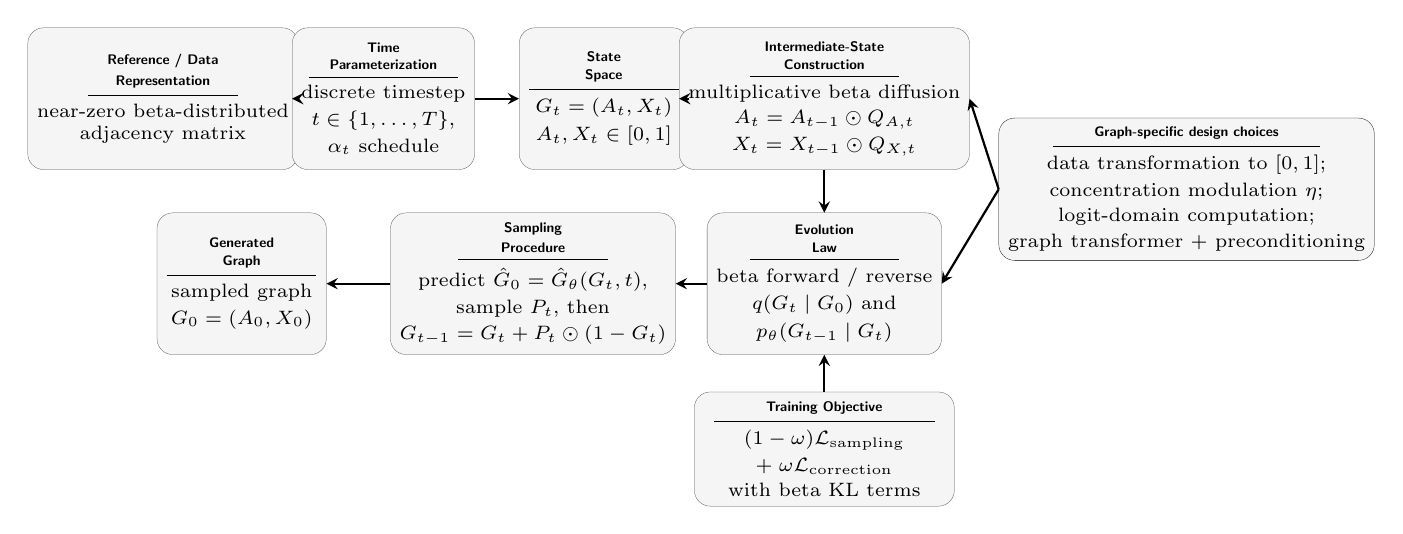
\begin{tikzpicture}[
    >=stealth,
    font=\scriptsize,
    box/.style={
        draw=black!70,
        rounded corners=2mm,
        ultra thin,
        minimum width=2.15cm,
        minimum height=1.8cm,
        align=center,
        fill=gray!8
    },
    side/.style={
        draw=black!70,
        rounded corners=2mm,
        ultra thin,
        minimum width=3.3cm,
        minimum height=1.45cm,
        align=center,
        fill=gray!8
    },
    note/.style={
        draw=black!70!black,
        rounded corners=2mm,
        ultra thin,
        minimum width=4.1cm,
        minimum height=1.8cm,
        align=center,
        fill=gray!8
    },
    arr/.style={->, thick}
]

% main pipeline: first row
\node[box] (base) at (0,0)
{\shortstack[c]{%
{\sffamily\bfseries\tiny Reference / Data}\\
{\sffamily\bfseries\tiny Representation}\\[-0.2mm]
\rule{1.9cm}{0.2pt}\\[0.0mm]
near-zero beta-distributed\\
adjacency matrix}};

\node[box] (time) at (2.8,0)
{\shortstack[c]{%
{\sffamily\bfseries\tiny Time}\\
{\sffamily\bfseries\tiny Parameterization}\\[-0.2mm]
\rule{1.9cm}{0.2pt}\\[0.0mm]
discrete timestep\\
$t\in\{1,\ldots,T\}$, \\$\alpha_t$ schedule}};

\node[box] (state) at (5.6,0)
{\shortstack[c]{%
{\sffamily\bfseries\tiny State}\\
{\sffamily\bfseries\tiny Space}\\[-0.2mm]
\rule{1.9cm}{0.2pt}\\[0.0mm]
$G_t=(A_t,X_t)$\\
$A_t,X_t\in[0,1]$}};

\node[box] (path) at (8.4,0)
{\shortstack[c]{%
{\sffamily\bfseries\tiny Intermediate-State}\\
{\sffamily\bfseries\tiny Construction}\\[-0.2mm]
\rule{1.9cm}{0.2pt}\\[0.0mm]
multiplicative beta diffusion\\
$A_t=A_{t-1}\odot Q_{A,t}$\\
$X_t=X_{t-1}\odot Q_{X,t}$}};

% second row
\node[box] (out) at (1.0,-2.35)
{\shortstack[c]{%
{\sffamily\bfseries\tiny Generated}\\
{\sffamily\bfseries\tiny Graph}\\[-0.2mm]
\rule{1.9cm}{0.2pt}\\[0.0mm]
sampled graph\\
$G_0=(A_0,X_0)$}};

\node[box] (sample) at (4.7,-2.35)
{\shortstack[c]{%
{\sffamily\bfseries\tiny Sampling}\\
{\sffamily\bfseries\tiny Procedure}\\[-0.2mm]
\rule{1.9cm}{0.2pt}\\[0.0mm]
predict $\hat G_0=\hat G_\theta(G_t,t)$,\\
sample $P_t$, then\\
$G_{t-1}=G_t+P_t\odot(1-G_t)$}};

\node[box] (evo) at (8.4,-2.35)
{\shortstack[c]{%
{\sffamily\bfseries\tiny Evolution}\\
{\sffamily\bfseries\tiny Law}\\[-0.2mm]
\rule{1.9cm}{0.2pt}\\[0.0mm]
beta forward / reverse\\
$q(G_t\mid G_0)$ and\\
$p_\theta(G_{t-1}\mid G_t)$}};

\draw[arr] (base) -- (time);
\draw[arr] (time) -- (state);
\draw[arr] (state) -- (path);
\draw[arr] (path.south) -- ++(0,-0.45) -| (evo.north);
\draw[arr] (evo) -- (sample);
\draw[arr] (sample) -- (out);

% side components
\node[side] (train) at (8.4,-4.45)
{\shortstack[c]{%
{\sffamily\bfseries\tiny Training Objective}\\[-0.2mm]
\rule{2.8cm}{0.2pt}\\[0.0mm]
$(1-\omega)\mathcal L_{\mathrm{sampling}}$\\
$+\;\omega\mathcal L_{\mathrm{correction}}$\\
with beta KL terms}};

\draw[arr] (train.north) -- (evo.south);

\node[note] (graphspec) at (13.0,-1.15)
{\shortstack[c]{%
{\sffamily\bfseries\tiny Graph-specific design choices}\\[-0.2mm]
\rule{3.4cm}{0.2pt}\\[0.0mm]
data transformation to $[0,1]$;\\
concentration modulation $\eta$;\\
logit-domain computation;\\
graph transformer + preconditioning}};

\draw[arr] (graphspec.west) -- (path.east);
\draw[arr] (graphspec.west) -- (evo.east);

\end{tikzpicture}
\caption{GBD pipeline. }
\label{fig:gbd_pipeline}
\end{figure*}

GBD is strong at modeling complex mixed node–edge dependencies through its joint beta diffusion process and can better align with sparse, bounded graph data than standard Gaussian or categorical noise, but it does not fundamentally resolve non-unique graph representations under permutation and still operates over a very large combinatorial output space. It also exposes limited interpretability or hard validity guarantees.


\emph{Evaluation.} GBD is a strong diffusion-based graph generator that improves distributional fit and graph-specific realism through beta diffusion and concentration modulation, but it still inherits core limitations of deep graph generation: non-canonical graph representations, largely implicit control of higher-order structure, and limited interpretability or hard validity guarantees.

\paragraph{Spectral diffusion.}
\emph{GGSD}~\cite{minello2024generating} takes an even more indirect route by performing denoising in a spectral representation of the graph Laplacian. Its diffusion path is defined over continuous spectral variables under Gaussian noising, and graph generation is obtained only after reconstructing the adjacency matrix from the denoised spectrum. Relative to GBD, the main shift is that the alternative representation is no longer bounded topology/attribute space but Laplacian spectral space, where the model can exploit global structural information more directly.

\begin{figure*}[htbp]
\centering
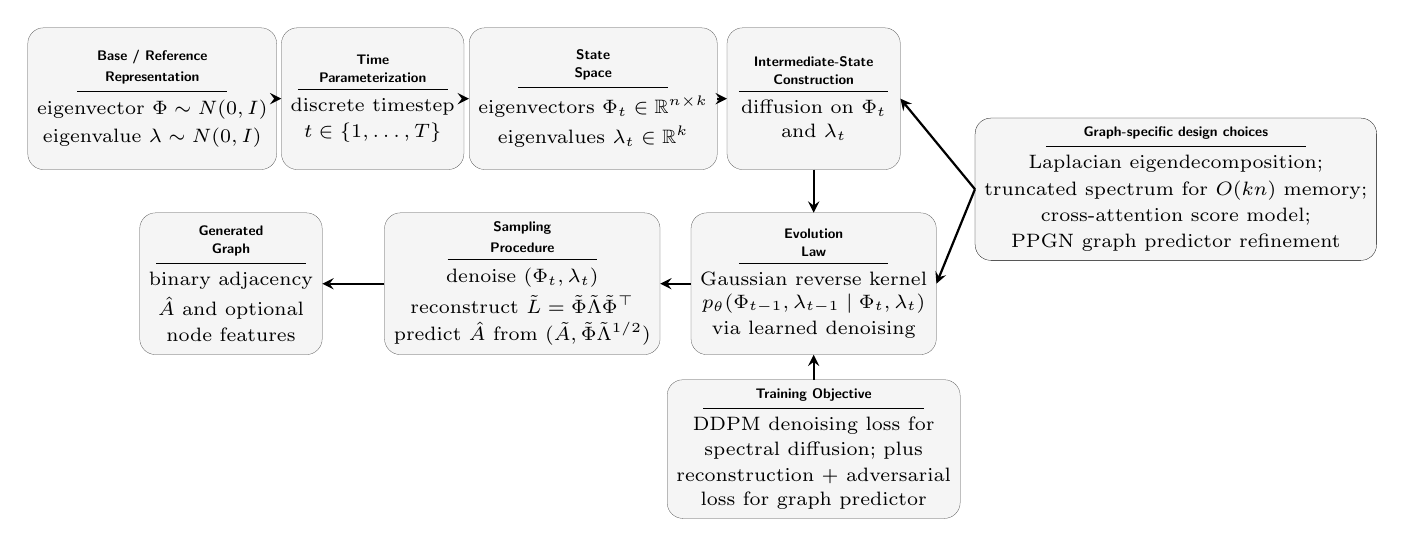
\begin{tikzpicture}[
    >=stealth,
    font=\scriptsize,
    box/.style={
        draw=black!70,
        rounded corners=2mm,
        ultra thin,
        minimum width=2.2cm,
        minimum height=1.8cm,
        align=center,
        fill=gray!8
    },
    side/.style={
        draw=black!70,
        rounded corners=2mm,
        ultra thin,
        minimum width=3.4cm,
        minimum height=1.45cm,
        align=center,
        fill=gray!8
    },
    note/.style={
        draw=black!70!black,
        rounded corners=2mm,
        ultra thin,
        minimum width=4.0cm,
        minimum height=1.75cm,
        align=center,
        fill=gray!8
    },
    arr/.style={->, thick}
]

% first row
\node[box] (base) at (0,0)
{\shortstack[c]{%
{\sffamily\bfseries\tiny Base / Reference}\\
{\sffamily\bfseries\tiny Representation}\\[-0.2mm]
\rule{1.9cm}{0.2pt}\\[0.0mm]
eigenvector $\Phi \sim N(0,I)$ \\
eigenvalue $\lambda \sim N(0,I)$ }};

\node[box] (time) at (2.8,0)
{\shortstack[c]{%
{\sffamily\bfseries\tiny Time}\\
{\sffamily\bfseries\tiny Parameterization}\\[-0.2mm]
\rule{1.9cm}{0.2pt}\\[0.0mm]
discrete timestep\\
$t\in\{1,\ldots,T\}$}};

\node[box] (state) at (5.6,0)
{\shortstack[c]{%
{\sffamily\bfseries\tiny State}\\
{\sffamily\bfseries\tiny Space}\\[-0.2mm]
\rule{1.9cm}{0.2pt}\\[0.0mm]
eigenvectors $\Phi_t\in\mathbb{R}^{n\times k}$\\
eigenvalues $\lambda_t\in\mathbb{R}^{k}$}};

\node[box] (path) at (8.4,0)
{\shortstack[c]{%
{\sffamily\bfseries\tiny Intermediate-State}\\
{\sffamily\bfseries\tiny Construction}\\[-0.2mm]
\rule{1.9cm}{0.2pt}\\[0.0mm]
diffusion on $\Phi_t$\\
and $\lambda_t$}};

% second row
\node[box] (out) at (1.0,-2.35)
{\shortstack[c]{%
{\sffamily\bfseries\tiny Generated}\\
{\sffamily\bfseries\tiny Graph}\\[-0.2mm]
\rule{1.9cm}{0.2pt}\\[0.0mm]
binary adjacency\\
$\hat A$ and optional\\
node features}};

\node[box] (sample) at (4.7,-2.35)
{\shortstack[c]{%
{\sffamily\bfseries\tiny Sampling}\\
{\sffamily\bfseries\tiny Procedure}\\[-0.2mm]
\rule{1.9cm}{0.2pt}\\[0.0mm]
denoise $(\Phi_t,\lambda_t)$\\
reconstruct $\tilde L=\tilde{\Phi}\tilde{\Lambda}\tilde{\Phi}^{\top}$\\
predict $\hat A$ from $(\tilde A,\tilde{\Phi}\tilde{\Lambda}^{1/2})$}};

\node[box] (evo) at (8.4,-2.35)
{\shortstack[c]{%
{\sffamily\bfseries\tiny Evolution}\\
{\sffamily\bfseries\tiny Law}\\[-0.2mm]
\rule{1.9cm}{0.2pt}\\[0.0mm]
Gaussian reverse kernel\\
$p_\theta(\Phi_{t-1},\lambda_{t-1}\mid \Phi_t,\lambda_t)$\\
via learned denoising}};

\draw[arr] (base) -- (time);
\draw[arr] (time) -- (state);
\draw[arr] (state) -- (path);
\draw[arr] (path.south) -- ++(0,-0.45) -| (evo.north);
\draw[arr] (evo) -- (sample);
\draw[arr] (sample) -- (out);

% side boxes
\node[side] (train) at (8.4,-4.45)
{\shortstack[c]{%
{\sffamily\bfseries\tiny Training Objective}\\[-0.2mm]
\rule{2.8cm}{0.2pt}\\[0.0mm]
DDPM denoising loss for\\
spectral diffusion; plus\\
reconstruction + adversarial\\
loss for graph predictor}};

\draw[arr] (train.north) -- (evo.south);

\node[note] (graphspec) at (13.0,-1.15)
{\shortstack[c]{%
{\sffamily\bfseries\tiny Graph-specific design choices}\\[-0.2mm]
\rule{3.3cm}{0.2pt}\\[0.0mm]
Laplacian eigendecomposition;\\
truncated spectrum for $O(kn)$ memory;\\
cross-attention score model;\\
PPGN graph predictor refinement}};

\draw[arr] (graphspec.west) -- (path.east);
\draw[arr] (graphspec.west) -- (evo.east);

\end{tikzpicture}
\caption{GGSD pipeline}
\label{fig:ggsd_pipeline}
\end{figure*}


\emph{Evaluation.} GGSD is particularly strong as a permutation-aware and scalable graph generator, because it shifts generation from adjacency space to Laplacian spectral space. This gives it a principled advantage on representation symmetry and computational efficiency, while also helping model global structure. Its main limitations are that validity and higher-order semantics are still controlled only indirectly, and the final generation pipeline remains partly black-box despite being more interpretable than many alternatives.


Overall, these representation-changing approaches broaden the design space of discrete-time denoising models. They show that the forward/reverse template is compatible not only with direct combinatorial corruption, but also with smoother bounded or spectral trajectories that may better capture global structure or mixed topology--attribute interactions.

\subsubsection{Hybrid absorbing and autoregressive models}
\label{sec:hybrid_absorbing_autoregressive_diffusion}



A third branch combines denoising-style refinement with \emph{structured generation order}. These models do not simply diffuse a full graph toward noise and reverse it symmetrically; instead, they embed denoising inside absorbing or autoregressive transition structures that impose a more explicit generation factorization.


\begin{figure*}[htbp]
\centering

%==================== GraphARM ====================
\begin{subfigure}[t]{\textwidth}
\centering
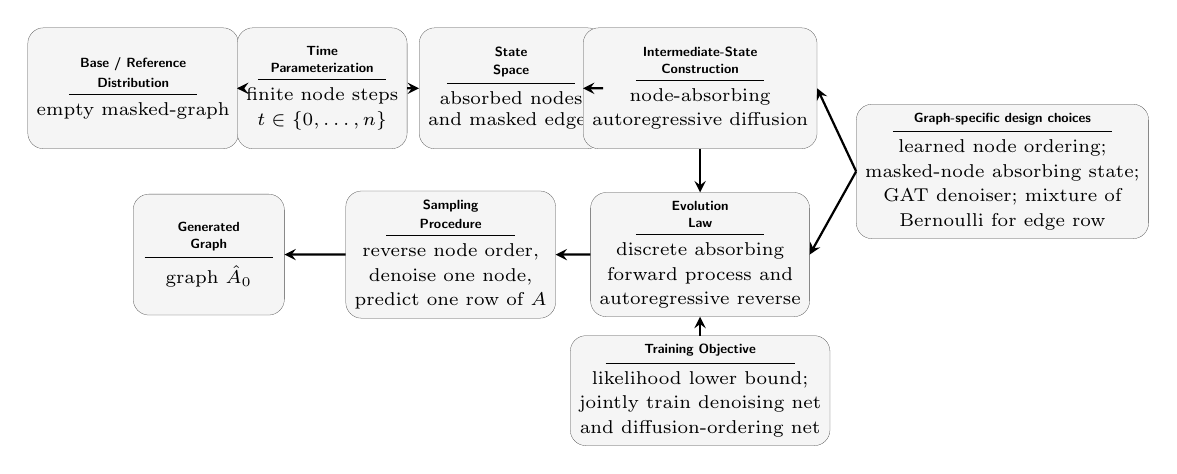
\begin{tikzpicture}[
    >=stealth,
    font=\scriptsize,
    scale=0.96,
    transform shape,
    box/.style={
        draw=black!70,
        rounded corners=2mm,
        ultra thin,
        minimum width=2.0cm,
        minimum height=1.6cm,
        align=center,
        fill=gray!8
    },
    side/.style={
        draw=black!70,
        rounded corners=2mm,
        ultra thin,
        minimum width=3.1cm,
        minimum height=1.2cm,
        align=center,
        fill=gray!8
    },
    note/.style={
        draw=black!70,
        rounded corners=2mm,
        ultra thin,
        minimum width=3.4cm,
        minimum height=1.45cm,
        align=center,
        fill=gray!8
    },
    arr/.style={->, thick}
]

% first row
\node[box] (base) at (0,0)
{\shortstack[c]{%
{\sffamily\bfseries\tiny Base / Reference}\\
{\sffamily\bfseries\tiny Distribution}\\[-0.2mm]
\rule{1.7cm}{0.2pt}\\[0.0mm]
empty masked-graph}};

\node[box] (time) at (2.5,0)
{\shortstack[c]{%
{\sffamily\bfseries\tiny Time}\\
{\sffamily\bfseries\tiny Parameterization}\\[-0.2mm]
\rule{1.7cm}{0.2pt}\\[0.0mm]
finite node steps\\
$t\in\{0,\ldots,n\}$}};

\node[box] (state) at (5.0,0)
{\shortstack[c]{%
{\sffamily\bfseries\tiny State}\\
{\sffamily\bfseries\tiny Space}\\[-0.2mm]
\rule{1.7cm}{0.2pt}\\[0.0mm]
absorbed nodes\\
and masked edges}};

\node[box] (path) at (7.5,0)
{\shortstack[c]{%
{\sffamily\bfseries\tiny Intermediate-State}\\
{\sffamily\bfseries\tiny Construction}\\[-0.2mm]
\rule{1.7cm}{0.2pt}\\[0.0mm]
node-absorbing\\
autoregressive diffusion}};

% second row
\node[box] (out) at (1.0,-2.2)
{\shortstack[c]{%
{\sffamily\bfseries\tiny Generated}\\
{\sffamily\bfseries\tiny Graph}\\[-0.2mm]
\rule{1.7cm}{0.2pt}\\[0.0mm]
graph $\hat A_0$}};

\node[box] (sample) at (4.2,-2.2)
{\shortstack[c]{%
{\sffamily\bfseries\tiny Sampling}\\
{\sffamily\bfseries\tiny Procedure}\\[-0.2mm]
\rule{1.7cm}{0.2pt}\\[0.0mm]
reverse node order,\\
denoise one node,\\
predict one row of $A$}};

\node[box] (evo) at (7.5,-2.2)
{\shortstack[c]{%
{\sffamily\bfseries\tiny Evolution}\\
{\sffamily\bfseries\tiny Law}\\[-0.2mm]
\rule{1.7cm}{0.2pt}\\[0.0mm]
discrete absorbing\\
forward process and\\
autoregressive reverse}};

\draw[arr] (base) -- (time);
\draw[arr] (time) -- (state);
\draw[arr] (state) -- (path);
\draw[arr] (path.south) -- ++(0,-0.4) -| (evo.north);
\draw[arr] (evo) -- (sample);
\draw[arr] (sample) -- (out);

% side boxes
\node[side] (train) at (7.5,-4.0)
{\shortstack[c]{%
{\sffamily\bfseries\tiny Training Objective}\\[-0.2mm]
\rule{2.5cm}{0.2pt}\\[0.0mm]
likelihood lower bound;\\
jointly train denoising net\\
and diffusion-ordering net}};

\draw[arr] (train.north) -- (evo.south);

\node[note] (graphspec) at (11.5,-1.1)
{\shortstack[c]{%
{\sffamily\bfseries\tiny Graph-specific design choices}\\[-0.2mm]
\rule{2.9cm}{0.2pt}\\[0.0mm]
learned node ordering;\\
masked-node absorbing state;\\
GAT denoiser; mixture of\\
Bernoulli for edge row}};

\draw[arr] (graphspec.west) -- (path.east);
\draw[arr] (graphspec.west) -- (evo.east);

\end{tikzpicture}
\caption{GraphARM.}
\label{fig:grapharm_pipeline}
\end{subfigure}

\vspace{0.8em}

%==================== LayerDAG ====================
\begin{subfigure}[t]{\textwidth}
\centering
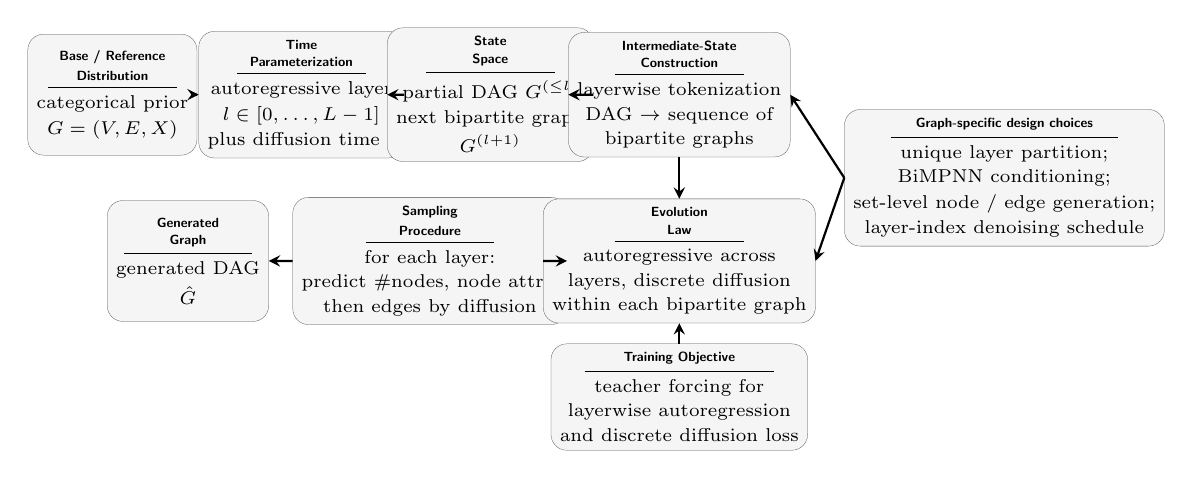
\begin{tikzpicture}[
    >=stealth,
    font=\scriptsize,
    scale=0.96,
    transform shape,
    box/.style={
        draw=black!70,
        rounded corners=2mm,
        ultra thin,
        minimum width=2.0cm,
        minimum height=1.6cm,
        align=center,
        fill=gray!8
    },
    side/.style={
        draw=black!70,
        rounded corners=2mm,
        ultra thin,
        minimum width=3.1cm,
        minimum height=1.2cm,
        align=center,
        fill=gray!8
    },
    note/.style={
        draw=black!70,
        rounded corners=2mm,
        ultra thin,
        minimum width=3.6cm,
        minimum height=1.45cm,
        align=center,
        fill=gray!8
    },
    arr/.style={->, thick}
]

% first row
\node[box] (base) at (0,0)
{\shortstack[c]{%
{\sffamily\bfseries\tiny Base / Reference}\\
{\sffamily\bfseries\tiny Distribution}\\[-0.2mm]
\rule{1.7cm}{0.2pt}\\[0.0mm]
categorical prior\\
$G=(V,E,X)$}};

\node[box] (time) at (2.5,0)
{\shortstack[c]{%
{\sffamily\bfseries\tiny Time}\\
{\sffamily\bfseries\tiny Parameterization}\\[-0.2mm]
\rule{1.7cm}{0.2pt}\\[0.0mm]
autoregressive layer\\
$l \in [0,\ldots,L-1]$\\
plus diffusion time $t$}};

\node[box] (state) at (5.0,0)
{\shortstack[c]{%
{\sffamily\bfseries\tiny State}\\
{\sffamily\bfseries\tiny Space}\\[-0.2mm]
\rule{1.7cm}{0.2pt}\\[0.0mm]
partial DAG $G^{(\leq l)}$\\
next bipartite graph\\
$G^{(l+1)}$}};

\node[box] (path) at (7.5,0)
{\shortstack[c]{%
{\sffamily\bfseries\tiny Intermediate-State}\\
{\sffamily\bfseries\tiny Construction}\\[-0.2mm]
\rule{1.7cm}{0.2pt}\\[0.0mm]
layerwise tokenization\\
DAG $\rightarrow$ sequence of\\
bipartite graphs}};

% second row
\node[box] (out) at (1.0,-2.2)
{\shortstack[c]{%
{\sffamily\bfseries\tiny Generated}\\
{\sffamily\bfseries\tiny Graph}\\[-0.2mm]
\rule{1.7cm}{0.2pt}\\[0.0mm]
generated DAG\\
$\hat G$}};

\node[box] (sample) at (4.2,-2.2)
{\shortstack[c]{%
{\sffamily\bfseries\tiny Sampling}\\
{\sffamily\bfseries\tiny Procedure}\\[-0.2mm]
\rule{1.7cm}{0.2pt}\\[0.0mm]
for each layer:\\
predict \#nodes, node attrs,\\
then edges by diffusion}};

\node[box] (evo) at (7.5,-2.2)
{\shortstack[c]{%
{\sffamily\bfseries\tiny Evolution}\\
{\sffamily\bfseries\tiny Law}\\[-0.2mm]
\rule{1.7cm}{0.2pt}\\[0.0mm]
autoregressive across\\
layers, discrete diffusion\\
within each bipartite graph}};

\draw[arr] (base) -- (time);
\draw[arr] (time) -- (state);
\draw[arr] (state) -- (path);
\draw[arr] (path.south) -- ++(0,-0.4) -| (evo.north);
\draw[arr] (evo) -- (sample);
\draw[arr] (sample) -- (out);

% side boxes
\node[side] (train) at (7.5,-4.0)
{\shortstack[c]{%
{\sffamily\bfseries\tiny Training Objective}\\[-0.2mm]
\rule{2.5cm}{0.2pt}\\[0.0mm]
teacher forcing for\\
layerwise autoregression\\
and discrete diffusion loss}};

\draw[arr] (train.north) -- (evo.south);

\node[note] (graphspec) at (11.8,-1.1)
{\shortstack[c]{%
{\sffamily\bfseries\tiny Graph-specific design choices}\\[-0.2mm]
\rule{3.0cm}{0.2pt}\\[0.0mm]
unique layer partition;\\
BiMPNN conditioning;\\
set-level node / edge generation;\\
layer-index denoising schedule}};

\draw[arr] (graphspec.west) -- (path.east);
\draw[arr] (graphspec.west) -- (evo.east);

\end{tikzpicture}
\caption{LayerDAG.}
\label{fig:layerdag_pipeline}
\end{subfigure}

\caption{Pipeline comparison of GraphARM and LayerDAG.}
\label{fig:grapharm_layerdag_pipelines}
\end{figure*}

\paragraph{Absorbing-order reverse generation.}
\emph{GraphARM}~\cite{kongautoregressive} uses a node-absorbing transition path together with autoregressive reverse reconstruction. Rather than treating all graph variables symmetrically at every step, it introduces a generation order through absorbing transitions and reconstructs the graph node by node in reverse. This places it between standard diffusion and autoregressive generation: it still uses a finite-step corruption/recovery logic, but the reverse process is organized around ordered node-wise prediction.

\emph{Evaluation.} GraphARM offers a useful compromise between efficiency, controllability, and discrete graph-space modeling: it improves over fixed-order autoregressive and one-shot diffusion baselines in handling ordering sensitivity and constraints, but it does not fully resolve permutation ambiguity, global-structure evaluation, or black-box reliability, and its nodewise sequential generation still faces the usual scalability and validity limitations of autoregressive graph models.

\paragraph{Layerwise DAG generation with inner denoising.}
\emph{LayerDAG}~\cite{li2024layerdag} is a hybrid discrete-time model specialized to DAG generation. Its outer process grows the graph layer by layer, while an inner discrete denoising process generates node attributes and edges within each bipartite layer transition. The resulting model therefore combines two forms of temporal structure: an autoregressive sequence over layers and a denoising refinement process within each local generation stage. Compared with GraphARM, the generation order is not node absorbing but DAG-layer based, and the architectural bias is tied directly to directional dependency structure.

\emph{Evaluation.} LayerDAG is stronger than GraphARM on representation symmetry, DAG-specific validity, and evaluation of implicit application-level properties, because it builds generation around a unique layerwise decomposition of DAGs and combines autoregression with diffusion at the right structural granularity.

These hybrid designs show that discrete-time denoising need not appear only as a full-graph corruption/recovery chain. It can also serve as a local refinement mechanism inside more structured autoregressive or absorbing generation schemes.

\subsection{Iterative Refinement and Editing-Based Methods}
\label{sec:dt_refinement}

Iterative refinement and editing-based methods model graph generation as a sequence of explicit graph modifications rather than as pure denoising from a fixed reference distribution. In this family, intermediate states are interpreted directly as editable graphs, and the main modeling questions concern what local edits are allowed, how they are scored or selected, and how refinement is guided by data likelihood, graph constraints, or critic-style feedback.

\begin{figure*}[htbp]
\centering
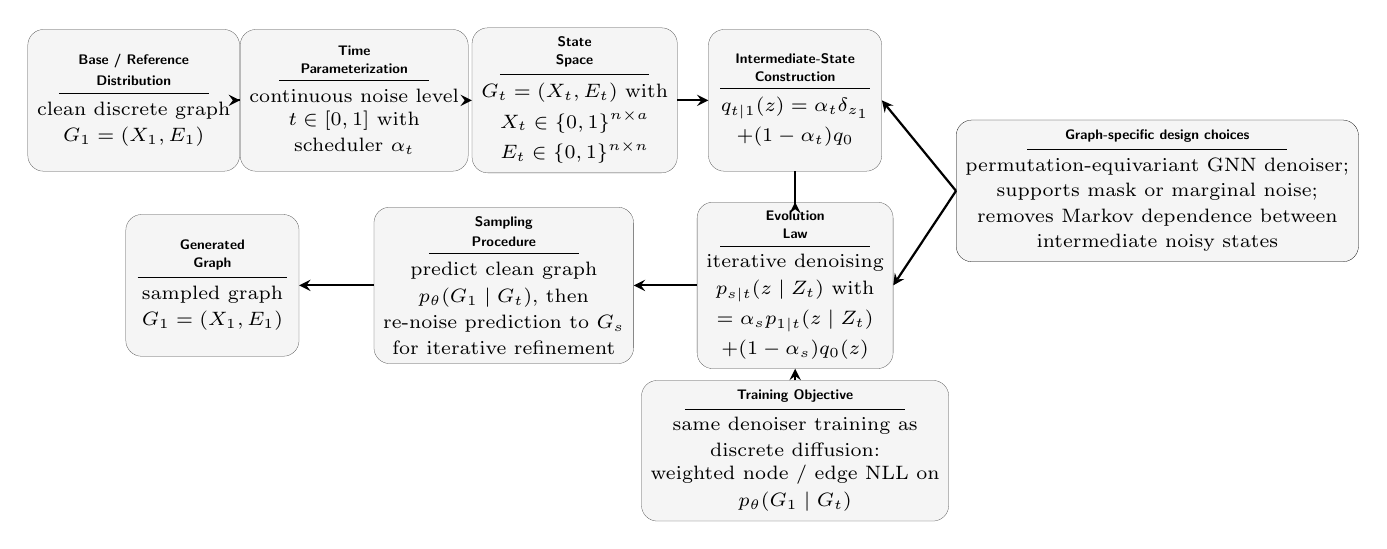
\begin{tikzpicture}[
    >=stealth,
    font=\scriptsize,
    box/.style={
        draw=black!70,
        rounded corners=2mm,
        ultra thin,
        minimum width=2.2cm,
        minimum height=1.8cm,
        align=center,
        fill=gray!8
    },
    side/.style={
        draw=black!70,
        rounded corners=2mm,
        ultra thin,
        minimum width=3.4cm,
        minimum height=1.45cm,
        align=center,
        fill=gray!8
    },
    note/.style={
        draw=black!70!black,
        rounded corners=2mm,
        ultra thin,
        minimum width=4.1cm,
        minimum height=1.8cm,
        align=center,
        fill=gray!8
    },
    arr/.style={->, thick}
]

% first row
\node[box] (base) at (0,0)
{\shortstack[c]{%
{\sffamily\bfseries\tiny Base / Reference}\\
{\sffamily\bfseries\tiny Distribution}\\[-0.2mm]
\rule{1.9cm}{0.2pt}\\[0.0mm]
clean discrete graph\\
$G_1=(X_1,E_1)$}};

\node[box] (time) at (2.8,0)
{\shortstack[c]{%
{\sffamily\bfseries\tiny Time}\\
{\sffamily\bfseries\tiny Parameterization}\\[-0.2mm]
\rule{1.9cm}{0.2pt}\\[0.0mm]
continuous noise level\\
$t\in[0,1]$ with\\
scheduler $\alpha_t$}};

\node[box] (state) at (5.6,0)
{\shortstack[c]{%
{\sffamily\bfseries\tiny State}\\
{\sffamily\bfseries\tiny Space}\\[-0.2mm]
\rule{1.9cm}{0.2pt}\\[0.0mm]
$G_t=(X_t,E_t)$ with\\
$X_t\in\{0,1\}^{n\times a}$ \\
$E_t\in\{0,1\}^{n\times n}$}};

\node[box] (path) at (8.4,0)
{\shortstack[c]{%
{\sffamily\bfseries\tiny Intermediate-State}\\
{\sffamily\bfseries\tiny Construction}\\[-0.2mm]
\rule{1.9cm}{0.2pt}\\[0.0mm]
$q_{t|1}(z)=\alpha_t\delta_{z_1}$\\ $+ (1-\alpha_t)q_0$}};

% second row
\node[box] (out) at (1.0,-2.35)
{\shortstack[c]{%
{\sffamily\bfseries\tiny Generated}\\
{\sffamily\bfseries\tiny Graph}\\[-0.2mm]
\rule{1.9cm}{0.2pt}\\[0.0mm]
sampled graph\\
$G_1=(X_1,E_1)$}};

\node[box] (sample) at (4.7,-2.35)
{\shortstack[c]{%
{\sffamily\bfseries\tiny Sampling}\\
{\sffamily\bfseries\tiny Procedure}\\[-0.2mm]
\rule{1.9cm}{0.2pt}\\[0.0mm]
predict clean graph\\
$p_\theta(G_1\mid G_t)$, then\\
re-noise prediction to $G_s$\\
for iterative refinement}};

\node[box] (evo) at (8.4,-2.35)
{\shortstack[c]{%
{\sffamily\bfseries\tiny Evolution}\\
{\sffamily\bfseries\tiny Law}\\[-0.2mm]
\rule{1.9cm}{0.2pt}\\[0.0mm]
iterative denoising\\
$p_{s|t}(z\mid Z_t)$ with\\
$=\alpha_s p_{1|t}(z\mid Z_t)$\\
$+(1-\alpha_s)q_0(z)$}};

\draw[arr] (base) -- (time);
\draw[arr] (time) -- (state);
\draw[arr] (state) -- (path);
\draw[arr] (path.south) -- ++(0,-0.45) -| (evo.north);
\draw[arr] (evo) -- (sample);
\draw[arr] (sample) -- (out);

% side boxes
\node[side] (train) at (8.4,-4.45)
{\shortstack[c]{%
{\sffamily\bfseries\tiny Training Objective}\\[-0.2mm]
\rule{2.8cm}{0.2pt}\\[0.0mm]
same denoiser training as\\
discrete diffusion:\\
weighted node / edge NLL on\\
$p_\theta(G_1\mid G_t)$}};

\draw[arr] (train.north) -- (evo.south);

\node[note] (graphspec) at (13.0,-1.15)
{\shortstack[c]{%
{\sffamily\bfseries\tiny Graph-specific design choices}\\[-0.2mm]
\rule{3.3cm}{0.2pt}\\[0.0mm]
permutation-equivariant GNN denoiser;\\
supports mask or marginal noise;\\
removes Markov dependence between\\
intermediate noisy states}}; 

\draw[arr] (graphspec.west) -- (path.east);
\draw[arr] (graphspec.west) -- (evo.east);

\end{tikzpicture}
\caption{SID pipeline}
\label{fig:sid_pipeline}
\end{figure*}

\emph{Simple Iterative Denoising} \cite{boget2025simple} (SID) handles permutation ambiguity better than order-based generators because it uses permutation-equivariant GNN denoisers and does not depend on a construction order, but it still does not remove non-unique graph representations entirely. It captures node-edge dependencies more coherently than standard discrete diffusion by repeatedly predicting a clean graph from noisy categorical node and edge states, though higher-order structure and global properties are still learned only implicitly rather than enforced directly. It also improves sampling over large graph spaces by reducing compounding denoising errors, but it does not fundamentally solve combinatorial scalability. SID is notably stronger on validity than standard discrete diffusion, especially for molecules, yet validity is still not guaranteed by construction for constraints such as connectivity or acyclicity. In terms of reliability, its predict-clean then re-noise rule is somewhat more interpretable than standard diffusion, but it remains a largely black-box neural generator.

\emph{Evaluation.} SID is particularly strong as a permutation-aware discrete graph generator because it uses permutation-equivariant denoisers and improves standard discrete diffusion by reducing compounding denoising errors through its predict-clean then re-noise mechanism. This gives it a practical advantage in sampling quality and validity, especially for molecular graphs, while retaining the flexibility of categorical node-edge generation. Its main limitations are that higher-order structure and global properties are still modeled only implicitly, validity is not guaranteed by construction, and the overall generation process remains only partially interpretable despite being clearer than standard discrete diffusion.


\subsection{Discrete Latent Transition Models}
\label{sec:dt_latent}

Discrete latent transition models place the main temporal process in a latent representation rather than directly in graph space. Compared with graph-space diffusion or editing models, these methods use a learned encoder--decoder architecture and define generation through staged latent decoding, hierarchical refinement, or latent-conditioned transitions that are later mapped back to graphs.


\emph{MAGNet} \cite{hetzel2025magnet} is best placed in the \emph{discrete latent-variable graph generation} family, since it generates molecules from a VAE latent space through a hierarchical coarse-to-fine decoding process rather than diffusion-style denoising. It therefore operates primarily in a \emph{latent space} and starts from a \emph{Gaussian prior} $p(z)=N(0,I)$. Unlike time-dependent generators, MAGNet does not introduce an explicit time parameterization; instead, its intermediate states are organized by hierarchical decoding stages, progressing from scaffold multiset and scaffold connectivity to motifs, join nodes, and leaf nodes. Its evolution law is thus given by a sequence of learned \emph{latent-conditioned decoding rules} for scaffold prediction, scaffold connectivity prediction, motif feature assignment, join-node identification, and leaf-node completion. The model is trained with a \emph{variational objective}, namely a VAE ELBO with reconstruction terms for scaffold- and atom-level components plus KL regularization toward the Gaussian prior, followed by a post-hoc normalizing flow to better align the latent distribution with the prior. Its main graph-specific design choices are \emph{hierarchical graph generation}, \emph{structural diversity} through scaffold abstraction and learned atom/bond assignment, and improved \emph{chemical validity and expressivity} through scaffold-based factorization.

\begin{figure*}[htbp]
\centering
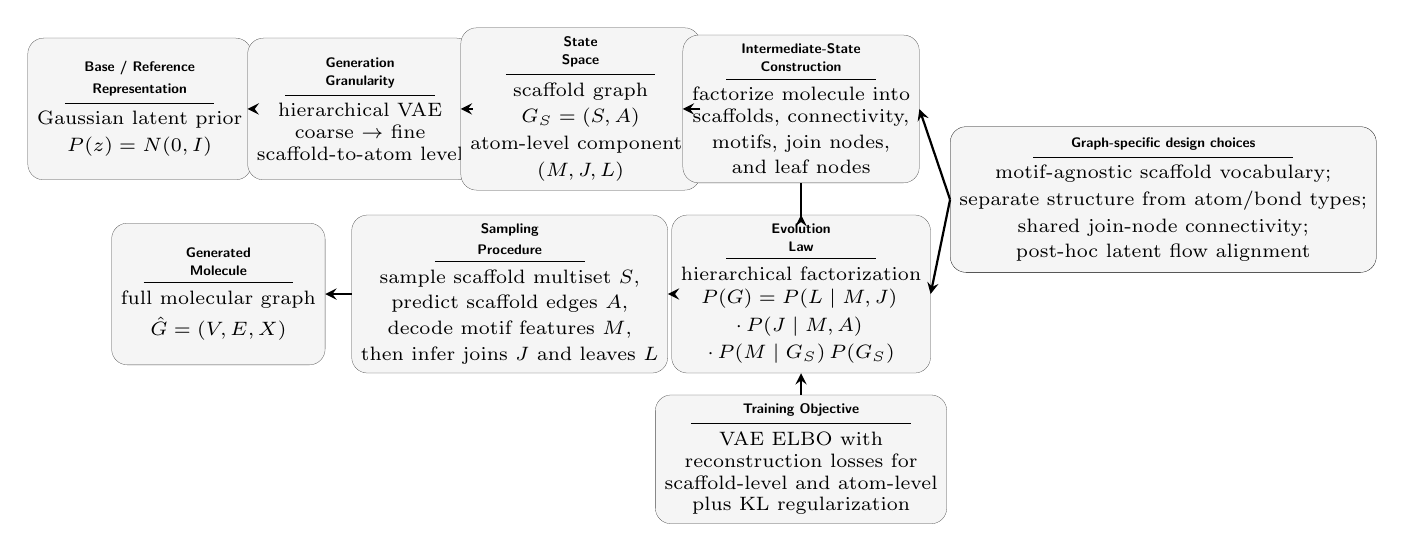
\begin{tikzpicture}[
    >=stealth,
    font=\scriptsize,
    box/.style={
        draw=black!70,
        rounded corners=2mm,
        ultra thin,
        minimum width=2.2cm,
        minimum height=1.8cm,
        align=center,
        fill=gray!8
    },
    side/.style={
        draw=black!70,
        rounded corners=2mm,
        ultra thin,
        minimum width=3.4cm,
        minimum height=1.45cm,
        align=center,
        fill=gray!8
    },
    note/.style={
        draw=black!70!black,
        rounded corners=2mm,
        ultra thin,
        minimum width=4.1cm,
        minimum height=1.85cm,
        align=center,
        fill=gray!8
    },
    arr/.style={->, thick}
]

% first row
\node[box] (base) at (0,0)
{\shortstack[c]{%
{\sffamily\bfseries\tiny Base / Reference}\\
{\sffamily\bfseries\tiny Representation}\\[-0.2mm]
\rule{1.9cm}{0.2pt}\\[0.0mm]
Gaussian latent prior\\
$P(z)=N(0,I)$}};

\node[box] (time) at (2.8,0)
{\shortstack[c]{%
{\sffamily\bfseries\tiny Generation}\\
{\sffamily\bfseries\tiny Granularity}\\[-0.2mm]
\rule{1.9cm}{0.2pt}\\[0.0mm]
hierarchical VAE\\
coarse $\rightarrow$ fine\\
scaffold-to-atom level}};

\node[box] (state) at (5.6,0)
{\shortstack[c]{%
{\sffamily\bfseries\tiny State}\\ 
{\sffamily\bfseries\tiny Space}\\[-0.2mm]
\rule{1.9cm}{0.2pt}\\[0.0mm]
scaffold graph\\
$G_S=(S,A)$\\
atom-level components\\
$(M,J,L)$}};

\node[box] (path) at (8.4,0)
{\shortstack[c]{%
{\sffamily\bfseries\tiny Intermediate-State}\\
{\sffamily\bfseries\tiny Construction}\\[-0.2mm]
\rule{1.9cm}{0.2pt}\\[0.0mm]
factorize molecule into\\
scaffolds, connectivity,\\
motifs, join nodes,\\
and leaf nodes}};

% second row
\node[box] (out) at (1.0,-2.35)
{\shortstack[c]{%
{\sffamily\bfseries\tiny Generated}\\
{\sffamily\bfseries\tiny Molecule}\\[-0.2mm]
\rule{1.9cm}{0.2pt}\\[0.0mm]
full molecular graph\\
$\hat G=(V,E,X)$}};

\node[box] (sample) at (4.7,-2.35)
{\shortstack[c]{%
{\sffamily\bfseries\tiny Sampling}\\
{\sffamily\bfseries\tiny Procedure}\\[-0.2mm]
\rule{1.9cm}{0.2pt}\\[0.0mm]
sample scaffold multiset $S$,\\
predict scaffold edges $A$,\\
decode motif features $M$,\\
then infer joins $J$ and leaves $L$}};

\node[box] (evo) at (8.4,-2.35)
{\shortstack[c]{%
{\sffamily\bfseries\tiny Evolution}\\
{\sffamily\bfseries\tiny Law}\\[-0.2mm]
\rule{1.9cm}{0.2pt}\\[0.0mm]
hierarchical factorization\\
$P(G)=P(L\mid M,J)\,$\\
$\cdot\,P(J\mid M,A)\,$\\
$\cdot\,P(M\mid G_S)\,P(G_S)$}};

\draw[arr] (base) -- (time);
\draw[arr] (time) -- (state);
\draw[arr] (state) -- (path);
\draw[arr] (path.south) -- ++(0,-0.45) -| (evo.north);
\draw[arr] (evo) -- (sample);
\draw[arr] (sample) -- (out);

% side boxes
\node[side] (train) at (8.4,-4.45)
{\shortstack[c]{%
{\sffamily\bfseries\tiny Training Objective}\\[-0.2mm]
\rule{2.8cm}{0.2pt}\\[0.0mm]
VAE ELBO with\\
reconstruction losses for\\
scaffold-level and atom-level\\
plus KL regularization}};

\draw[arr] (train.north) -- (evo.south);

\node[note] (graphspec) at (13.0,-1.15)
{\shortstack[c]{%
{\sffamily\bfseries\tiny Graph-specific design choices}\\[-0.2mm]
\rule{3.3cm}{0.2pt}\\[0.0mm]
motif-agnostic scaffold vocabulary;\\
separate structure from atom/bond types;\\
shared join-node connectivity;\\
post-hoc latent flow alignment}}; 

\draw[arr] (graphspec.west) -- (path.east);
\draw[arr] (graphspec.west) -- (evo.east);

\end{tikzpicture}
\caption{MAGNet pipeline.}
\label{fig:magnet_pipeline}
\end{figure*}

\emph{Evaluation.} MAGNet is particularly strong because it reframes molecular generation around scaffold structure rather than fixed motif vocabularies. This gives it a better handle on structural diversity, feature allocation, and evaluation beyond standard benchmarks. Its main remaining limitations are that it is still a learned hierarchical VAE rather than a fully interpretable or formally constrained generator, and its representation advances are more about molecular abstraction than about solving graph symmetry in full generality.


\label{sec:dt_summary}


% =========================
% =========================






\section{Continuous-Time Graph Generation}
\label{sec:continuous_time}


\begin{figure*}[!htbp]
\centering
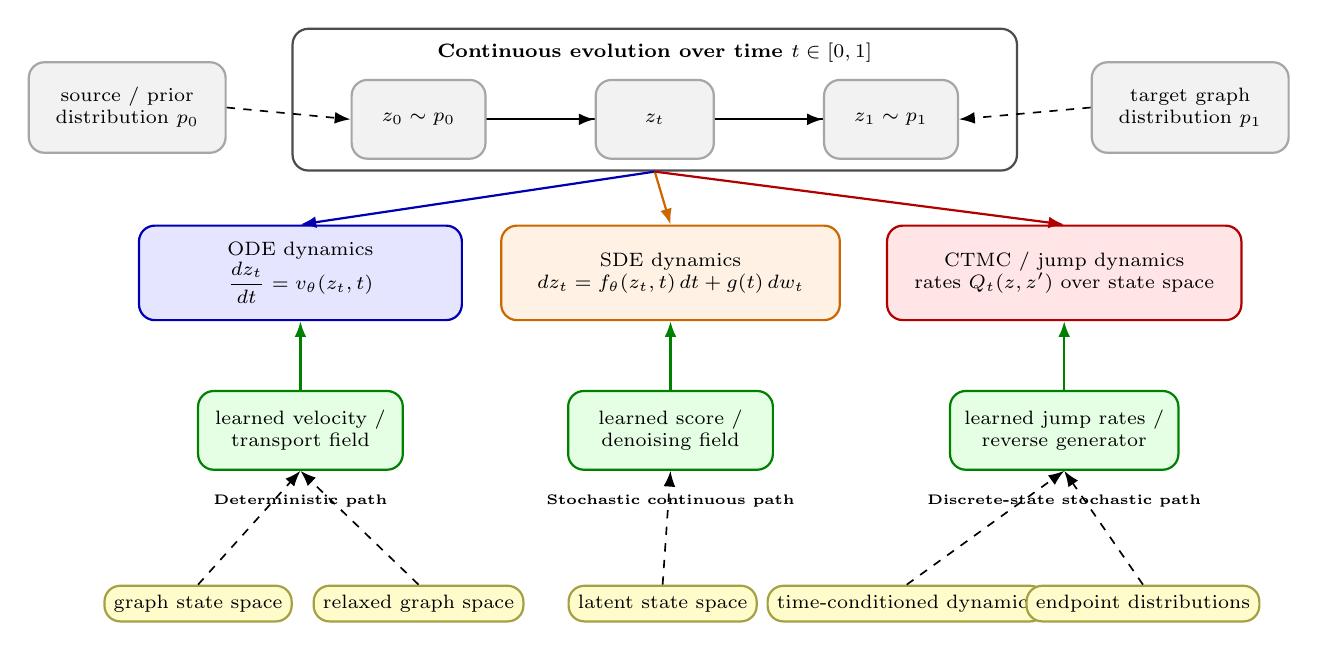
\begin{tikzpicture}[
    >=Latex,
    font=\sffamily,
    state/.style={
        draw=gray!70,
        rounded corners=2mm,
        thick,
        minimum width=2.1cm,
        minimum height=1.0cm,
        align=center,
        fill=gray!10,
        font=\scriptsize
    },
    timelinebox/.style={
        draw=black!70,
        rounded corners=2mm,
        thick,
        minimum width=9.2cm,
        minimum height=1.8cm,
        align=center,
        fill=white
    },
    sidebox/.style={
        draw=blue!70!black,
        rounded corners=2mm,
        thick,
        minimum width=4.1cm,
        minimum height=1.2cm,
        align=center,
        fill=blue!10,
        font=\scriptsize
    },
    orangebox/.style={
        draw=orange!80!black,
        rounded corners=2mm,
        thick,
        minimum width=4.3cm,
        minimum height=1.2cm,
        align=center,
        fill=orange!10,
        font=\scriptsize
    },
    redbox/.style={
        draw=red!70!black,
        rounded corners=2mm,
        thick,
        minimum width=4.5cm,
        minimum height=1.2cm,
        align=center,
        fill=red!10,
        font=\scriptsize
    },
    greenbox/.style={
        font=\scriptsize,
        draw=green!50!black,
        rounded corners=2mm,
        thick,
        minimum width=2.6cm,
        minimum height=1.0cm,
        align=center,
        fill=green!10
    },
    note/.style={
        draw=yellow!60!black,
        rounded corners=2mm,
        thick,
        font=\scriptsize,
        minimum width=1.7cm,
        minimum height=0.45cm,
        align=center,
        fill=yellow!20
    },
    blueaux/.style={blue!70!black, thick, -{Latex[length=2mm]}},
    orangeaux/.style={orange!80!black, thick, -{Latex[length=2mm]}},
    redaux/.style={red!70!black, thick, -{Latex[length=2mm]}},
    greenaux/.style={green!50!black, thick, -{Latex[length=2mm]}},
    goldaux/.style={
        dashed,
        semithick,
        -{Latex[length=2mm]}
    },
    blackaux/.style={
        black,
        thick,
        -{Latex[length=2mm]}
    }
]

% endpoint distributions
\node[state, minimum width=2.5cm, minimum height=1.15cm] (p0) at (1.3,7.0)
{source / prior\\distribution $p_0$};

\node[state, minimum width=2.5cm, minimum height=1.15cm] (p1) at (14.8,7.0)
{target graph\\distribution $p_1$};

% enclosing timeline box
\node[timelinebox] (tbox) at (8.0,7.1) {};

% title inside timeline box
\node[font=\bfseries\scriptsize] at (8.0,7.7)
{Continuous evolution over time $t \in [0,1]$};

% horizontal timeline
\draw[black, thick] (5.2,6.85) -- (10.8,6.85);

% ticks
\draw[black, thick] (5.35,6.67) -- (5.35,7.03);
\draw[black, thick] (10.65,6.67) -- (10.65,7.03);

\node[font=\scriptsize] at (5.35,7.18) {$0$};
\node[font=\scriptsize] at (10.65,7.18) {$1$};

% states on the path
\node[state, minimum width=1.7cm, minimum height=1.0cm] (z0) at (5.0,6.85)
{$z_0 \sim p_0$};

\node[state, minimum width=1.5cm, minimum height=1.0cm] (zt) at (8.0,6.85)
{$z_t$};

\node[state, minimum width=1.7cm, minimum height=1.0cm] (z1) at (11.0,6.85)
{$z_1 \sim p_1$};

% trajectory arrows
\draw[blackaux] (z0.east) -- (zt.west);
\draw[blackaux] (zt.east) -- (z1.west);

% endpoint distribution arrows
\draw[goldaux] (p0.east) -- (z0.west);
\draw[goldaux] (p1.west) -- (z1.east);

% dynamics families
\node[sidebox] (ode) at (3.5,4.9)
{ODE dynamics\\$\dfrac{dz_t}{dt}=v_\theta(z_t,t)$};

\node[orangebox] (sde) at (8.2,4.9)
{SDE dynamics\\$dz_t=f_\theta(z_t,t)\,dt+g(t)\,dw_t$};

\node[redbox] (ctmc) at (13.2,4.9)
{CTMC / jump dynamics\\rates $Q_t(z,z')$ over state space};

% connect timeline to dynamics
\draw[blueaux] (tbox.south) -- (ode.north);
\draw[orangeaux] (tbox.south) -- (sde.north);
\draw[redaux] (tbox.south) -- (ctmc.north);

% learned objects
\node[greenbox] (vel) at (3.5,2.9)
{learned velocity /\\transport field};

\node[greenbox] (score) at (8.2,2.9)
{learned score /\\denoising field};

\node[greenbox, minimum width=2.9cm] (jump) at (13.2,2.9)
{learned jump rates /\\reverse generator};

\draw[greenaux] (vel.north) -- (ode.south);
\draw[greenaux] (score.north) -- (sde.south);
\draw[greenaux] (jump.north) -- (ctmc.south);

% labels under dynamics
\node[font=\bfseries\tiny] at (3.5,2.0) {Deterministic path};
\node[font=\bfseries\tiny] at (8.2,2.0) {Stochastic continuous path};
\node[font=\bfseries\tiny] at (13.2,2.0) {Discrete-state stochastic path};

% notes
\node[note, minimum width=2.2cm] (n1) at (2.2,0.7)
{graph state space};

\node[note, minimum width=2.2cm] (n2) at (5.0,0.7)
{relaxed graph space};

\node[note, minimum width=2.2cm] (n3) at (8.1,0.7)
{latent state space};

\node[note, minimum width=2.5cm] (n4) at (11.2,0.7)
{time-conditioned dynamics};

\node[note, minimum width=2.2cm] (n5) at (14.2,0.7)
{endpoint distributions};

\draw[goldaux] (n1.north) -- (vel.south);
\draw[goldaux] (n2.north) -- (vel.south);
\draw[goldaux] (n3.north) -- (score.south);
\draw[goldaux] (n4.north) -- (jump.south);
\draw[goldaux] (n5.north) -- (jump.south);

\end{tikzpicture}
\caption{Generic architecture of continuous-time graph generation.}
\label{fig:generic_continuous_time_architecture}
\end{figure*}

Continuous-time graph generation models the generative process as an evolution over a continuous time variable $t \in [0,1]$, rather than as a finite sequence of discrete transitions. This perspective unifies several important families of methods, including deterministic ODE-based transport models, stochastic SDE-based diffusion and score models, discrete-state continuous-time jump processes, and bridge-based formulations. Although these families differ substantially in their mathematical form, they share a common viewpoint: graph generation is described through a time-indexed trajectory between an initial reference distribution and a target graph distribution, together with a learned evolution law that governs how states move along this trajectory. The main design differences therefore concern the type of dynamics, the state space in which evolution is defined, the construction of intermediate probability paths, and the graph-specific mechanisms used to preserve structure, validity, and permutation symmetry. Figure~\ref{fig:generic_continuous_time_architecture} summarizes this common template, and Table~\ref{tab:continuous_time_models} provides a compact overview of the representative models discussed in this section.




\begin{table*}[http]
\centering
\footnotesize
\renewcommand{\arraystretch}{1.1}
\setlength{\tabcolsep}{4pt}
\begin{tabularx}{\textwidth}{@{}
>{\raggedright\arraybackslash}p{1.6cm}
>{\raggedright\arraybackslash}p{2.8cm}
>{\raggedright\arraybackslash}p{2.2cm}
>{\raggedright\arraybackslash}p{2.6cm}
>{\raggedright\arraybackslash}X
@{}}
\toprule
\textbf{Model} & \textbf{Family} & \textbf{Space} & \textbf{Path / Dynamics} & \textbf{Key idea} \\
\midrule
CGF       & ODE / CNF                  & relaxed graph     & neural ODE transport            & exact-likelihood continuous graph flow \\
ModFlow   & ODE / CNF                  & relaxed graph     & coupled node ODE                & equivariant molecular flow \\
CatFlow   & flow matching              & relaxed graph     & conditional interpolation       & categorical flow matching \\
GGFlow    & discrete flow matching     & discrete graph    & jump-style conditional path     & sparse prior and conditional flow \\
DeFoG     & discrete flow matching     & discrete graph    & linear path + CTMC reverse      & discrete denoising flow matching \\
BWFlow    & geometry-aware transport   & relaxed graph     & Bures--Wasserstein path         & graph-aware interpolation geometry \\
GGBall    & geometry-aware transport   & hyperbolic latent & geodesic interpolation          & curvature-aware latent graph transport \\
EDP-GNN   & score-based / diffusion    & relaxed adjacency & Gaussian perturbation           & permutation-equivariant score model \\
PRODIGY   & SDE / constrained sampling & relaxed graph     & reverse diffusion + projection  & plug-and-play constraint control \\
GraphBSI  & SDE / belief-space         & relaxed belief    & stochastic belief evolution     & categorical belief-space generation \\
DisCo     & CTMC                       & discrete graph    & continuous-time jump process    & direct discrete-state graph diffusion \\
GruM      & bridge-based               & relaxed graph     & OU bridge mixture               & endpoint-conditioned stochastic transport \\
\bottomrule
\end{tabularx}
\caption{Representative continuous-time graph generation models.}
\label{tab:continuous_time_models}
\end{table*}

\subsection{ODE-Based Deterministic Models}
\label{sec:ode_models}

ODE-based deterministic models generate graphs by transporting a base distribution to the data distribution through a continuous-time velocity field. In graph domains, these methods are most natural when the evolving state is a continuous latent representation or a continuous relaxation of graph variables, since standard ODE dynamics do not act directly on discrete combinatorial graph states. Within this family, we distinguish four main directions: continuous normalizing flows, flow-matching-based methods, rectified-flow-style simplifications, and geometry-aware transport constructions. The main design choices concern the representation in which transport is defined, the construction of intermediate paths, and the way graph structure is preserved or recovered along the trajectory.

\paragraph{Continuous normalizing flows.}
Continuous normalizing flows define generation through an invertible ODE transport from a simple base distribution to a target graph distribution. In graph generation, they are especially natural when graphs are represented in continuous node, edge, or latent variables and later decoded into discrete structures.

\begin{figure*}[htbp]
\centering

% =========================
% Subfigure (a): CGF
% =========================
\begin{subfigure}[t]{\textwidth}
\centering
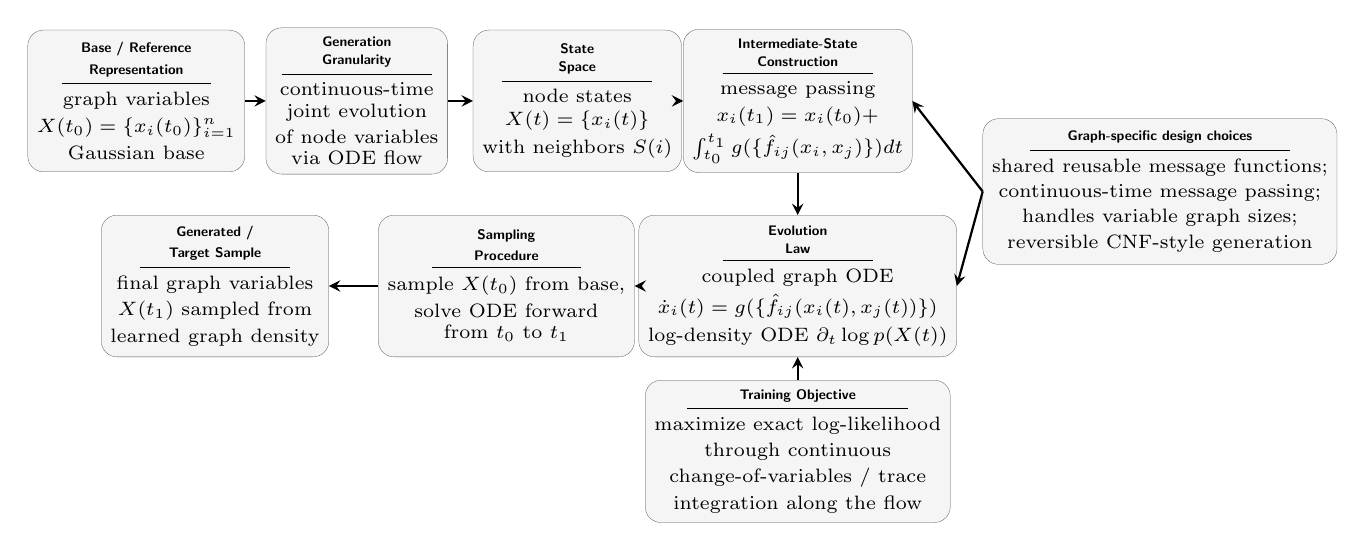
\begin{tikzpicture}[
    >=stealth,
    font=\scriptsize,
    box/.style={
        draw=black!70,
        rounded corners=2mm,
        ultra thin,
        minimum width=2.2cm,
        minimum height=1.8cm,
        align=center,
        fill=gray!8
    },
    side/.style={
        draw=black!70,
        rounded corners=2mm,
        ultra thin,
        minimum width=3.4cm,
        minimum height=1.45cm,
        align=center,
        fill=gray!8
    },
    note/.style={
        draw=black!70,
        rounded corners=2mm,
        ultra thin,
        minimum width=4.1cm,
        minimum height=1.85cm,
        align=center,
        fill=gray!8
    },
    arr/.style={->, thick}
]

% first row
\node[box] (base) at (0,0)
{\shortstack[c]{%
{\sffamily\bfseries\tiny Base / Reference}\\
{\sffamily\bfseries\tiny Representation}\\[-0.2mm]
\rule{1.9cm}{0.2pt}\\[0.0mm]
graph variables\\
$X(t_0)=\{x_i(t_0)\}_{i=1}^n$\\
Gaussian base}};

\node[box] (time) at (2.8,0)
{\shortstack[c]{%
{\sffamily\bfseries\tiny Generation}\\
{\sffamily\bfseries\tiny Granularity}\\[-0.2mm]
\rule{1.9cm}{0.2pt}\\[0.0mm]
continuous-time\\
joint evolution\\
of node variables\\
via ODE flow}};

\node[box] (state) at (5.6,0)
{\shortstack[c]{%
{\sffamily\bfseries\tiny State}\\
{\sffamily\bfseries\tiny Space}\\[-0.2mm]
\rule{1.9cm}{0.2pt}\\[0.0mm]
node states\\
$X(t)=\{x_i(t)\}$\\
with neighbors $S(i)$}};

\node[box] (path) at (8.4,0)
{\shortstack[c]{%
{\sffamily\bfseries\tiny Intermediate-State}\\
{\sffamily\bfseries\tiny Construction}\\[-0.2mm]
\rule{1.9cm}{0.2pt}\\[0.0mm]
message passing\\
$x_i(t_1)=x_i(t_0)+$\\
$\int_{t_0}^{t_1} g(\{\hat f_{ij}(x_i,x_j)\})dt$}};

% second row
\node[box] (out) at (1.0,-2.35)
{\shortstack[c]{%
{\sffamily\bfseries\tiny Generated /}\\
{\sffamily\bfseries\tiny Target Sample}\\[-0.2mm]
\rule{1.9cm}{0.2pt}\\[0.0mm]
final graph variables\\
$X(t_1)$ sampled from\\
learned graph density}};

\node[box] (sample) at (4.7,-2.35)
{\shortstack[c]{%
{\sffamily\bfseries\tiny Sampling}\\
{\sffamily\bfseries\tiny Procedure}\\[-0.2mm]
\rule{1.9cm}{0.2pt}\\[0.0mm]
sample $X(t_0)$ from base,\\
solve ODE forward\\
from $t_0$ to $t_1$}};

\node[box] (evo) at (8.4,-2.35)
{\shortstack[c]{%
{\sffamily\bfseries\tiny Evolution}\\
{\sffamily\bfseries\tiny Law}\\[-0.2mm]
\rule{1.9cm}{0.2pt}\\[0.0mm]
coupled graph ODE\\
$\dot x_i(t)=g(\{\hat f_{ij}(x_i(t),x_j(t))\})$\\
log-density ODE
$\partial_t \log p(X(t))$}};

\draw[arr] (base) -- (time);
\draw[arr] (time) -- (state);
\draw[arr] (state) -- (path);
\draw[arr] (path.south) -- ++(0,-0.45) -| (evo.north);
\draw[arr] (evo) -- (sample);
\draw[arr] (sample) -- (out);

% side boxes
\node[side] (train) at (8.4,-4.45)
{\shortstack[c]{%
{\sffamily\bfseries\tiny Training Objective}\\[-0.2mm]
\rule{2.8cm}{0.2pt}\\[0.0mm]
maximize exact log-likelihood\\
through continuous\\
change-of-variables / trace\\
integration along the flow}};

\draw[arr] (train.north) -- (evo.south);

\node[note] (graphspec) at (13.0,-1.15)
{\shortstack[c]{%
{\sffamily\bfseries\tiny Graph-specific design choices}\\[-0.2mm]
\rule{3.3cm}{0.2pt}\\[0.0mm]
shared reusable message functions;\\
continuous-time message passing;\\
handles variable graph sizes;\\
reversible CNF-style generation}}; 

\draw[arr] (graphspec.west) -- (path.east);
\draw[arr] (graphspec.west) -- (evo.east);

\end{tikzpicture}
\caption{Continuous Graph Flow (CGF).}
\end{subfigure}

\vspace{0.8em}

% =========================
% Subfigure (b): ModFlow
% =========================
\begin{subfigure}[t]{\textwidth}
\centering
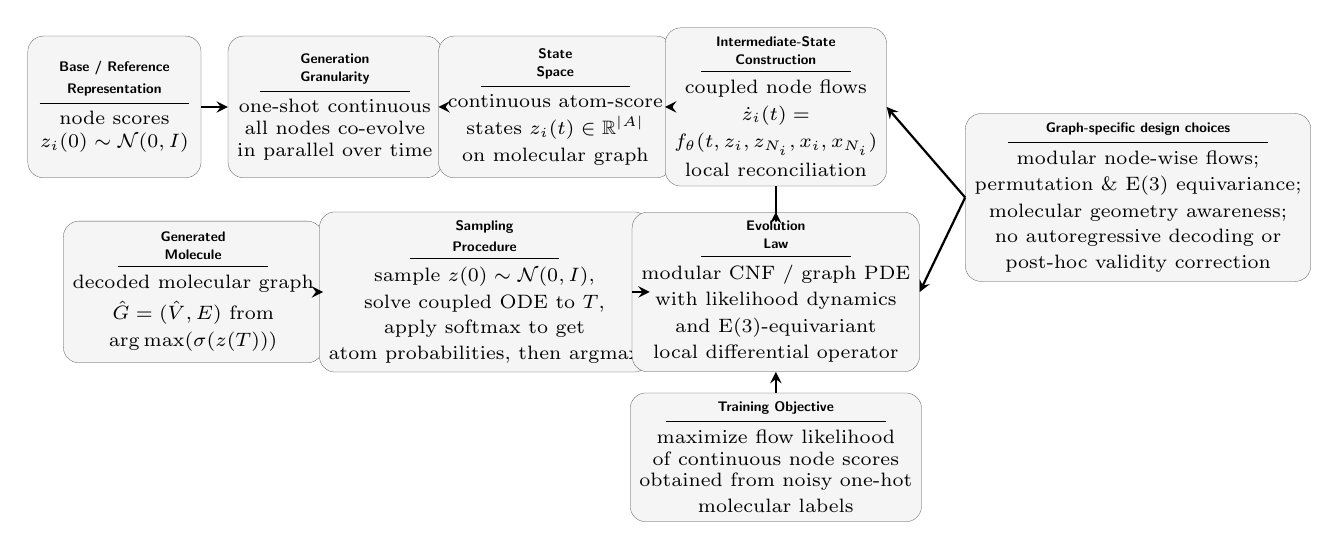
\begin{tikzpicture}[
    >=stealth,
    font=\scriptsize,
    box/.style={
        draw=black!70,
        rounded corners=2mm,
        ultra thin,
        minimum width=2.2cm,
        minimum height=1.8cm,
        align=center,
        fill=gray!8
    },
    side/.style={
        draw=black!70,
        rounded corners=2mm,
        ultra thin,
        minimum width=3.4cm,
        minimum height=1.45cm,
        align=center,
        fill=gray!8
    },
    note/.style={
        draw=black!70,
        rounded corners=2mm,
        ultra thin,
        minimum width=4.1cm,
        minimum height=1.85cm,
        align=center,
        fill=gray!8
    },
    arr/.style={->, thick}
]

% first row
\node[box] (base) at (0,0)
{\shortstack[c]{%
{\sffamily\bfseries\tiny Base / Reference}\\
{\sffamily\bfseries\tiny Representation}\\[-0.2mm]
\rule{1.9cm}{0.2pt}\\[0.0mm]
 node scores \\ $z_i(0)\sim\mathcal N(0,I)$}};

\node[box] (time) at (2.8,0)
{\shortstack[c]{%
{\sffamily\bfseries\tiny Generation}\\
{\sffamily\bfseries\tiny Granularity}\\[-0.2mm]
\rule{1.9cm}{0.2pt}\\[0.0mm]
one-shot continuous\\
all nodes co-evolve\\
in parallel over time}};

\node[box] (state) at (5.6,0)
{\shortstack[c]{%
{\sffamily\bfseries\tiny State}\\
{\sffamily\bfseries\tiny Space}\\[-0.2mm]
\rule{1.9cm}{0.2pt}\\[0.0mm]
continuous atom-score\\
states $z_i(t)\in\mathbb R^{|A|}$\\
on molecular graph }};

\node[box] (path) at (8.4,0)
{\shortstack[c]{%
{\sffamily\bfseries\tiny Intermediate-State}\\
{\sffamily\bfseries\tiny Construction}\\[-0.2mm]
\rule{1.9cm}{0.2pt}\\[0.0mm]
coupled node flows\\
$\dot z_i(t)=$ \\$f_\theta(t,z_i,z_{N_i},x_i,x_{N_i})$\\
local reconciliation }};

% second row
\node[box] (out) at (1.0,-2.35)
{\shortstack[c]{%
{\sffamily\bfseries\tiny Generated}\\
{\sffamily\bfseries\tiny Molecule}\\[-0.2mm]
\rule{1.9cm}{0.2pt}\\[0.0mm]
decoded molecular graph\\
$\hat G=(\hat V,E)$ from\\
$\arg\max(\sigma(z(T)))$}};

\node[box] (sample) at (4.7,-2.35)
{\shortstack[c]{%
{\sffamily\bfseries\tiny Sampling}\\
{\sffamily\bfseries\tiny Procedure}\\[-0.2mm]
\rule{1.9cm}{0.2pt}\\[0.0mm]
sample $z(0)\sim\mathcal N(0,I)$,\\
solve coupled ODE to $T$,\\
apply softmax to get\\
atom probabilities, then argmax}};

\node[box] (evo) at (8.4,-2.35)
{\shortstack[c]{%
{\sffamily\bfseries\tiny Evolution}\\
{\sffamily\bfseries\tiny Law}\\[-0.2mm]
\rule{1.9cm}{0.2pt}\\[0.0mm]
modular CNF / graph PDE\\
with likelihood dynamics\\
and E(3)-equivariant\\
local differential operator}};

\draw[arr] (base) -- (time);
\draw[arr] (time) -- (state);
\draw[arr] (state) -- (path);
\draw[arr] (path.south) -- ++(0,-0.45) -| (evo.north);
\draw[arr] (evo) -- (sample);
\draw[arr] (sample) -- (out);

% side boxes
\node[side] (train) at (8.4,-4.45)
{\shortstack[c]{%
{\sffamily\bfseries\tiny Training Objective}\\[-0.2mm]
\rule{2.8cm}{0.2pt}\\[0.0mm]
maximize flow likelihood\\
of continuous node scores\\
obtained from noisy one-hot\\
molecular labels}};

\draw[arr] (train.north) -- (evo.south);

\node[note] (graphspec) at (13.0,-1.15)
{\shortstack[c]{%
{\sffamily\bfseries\tiny Graph-specific design choices}\\[-0.2mm]
\rule{3.3cm}{0.2pt}\\[0.0mm]
modular node-wise flows;\\
permutation \& E(3) equivariance;\\
molecular geometry awareness;\\
no autoregressive decoding or\\
post-hoc validity correction}}; 

\draw[arr] (graphspec.west) -- (path.east);
\draw[arr] (graphspec.west) -- (evo.east);

\end{tikzpicture}
\caption{Modular Flows (ModFlow).}
\end{subfigure}

\caption{Pipelines of two continuous-time flow-based graph generators. Top: Continuous Graph Flow (CGF). Bottom: ModFlow.}
\label{fig:cgf_modflow_pipelines}
\end{figure*}
\emph{Continuous Graph Flow} (CGF) \cite{deng2019continuous} is an \emph{ODE-based continuous normalizing flow} that generates graphs in a \emph{relaxed continuous space}. It begins from a \emph{Gaussian base distribution} and transports samples through a deterministic continuous-time message-passing dynamics defined by a learned graph-structured \emph{velocity field}. Likelihood is computed with the continuous change-of-variables formula, while binary graph variables are handled by variational dequantization. Trained by \emph{maximum likelihood} and sampled by ODE integration, CGF supports variable-size graphs, permutation-equivariant relational modeling, and avoids any fixed autoregressive ordering.

CGF is strong at modeling complex dependencies and handling large output spaces because it replaces discrete graph construction with continuous transport driven by graph-structured message passing, allowing rich relational interactions without a fixed autoregressive order. It also partly alleviates non-unique representations through permutation-equivariant message passing and order-free generation, though it still depends on a chosen graph representation rather than fully resolving permutation ambiguity. Its main limitations are that implicit global properties and domain-specific validity constraints are handled only indirectly, and despite its principled ODE likelihood formulation, the learned continuous transport remains relatively black-box and not easily interpretable or controllable.




\emph{ModFlow} \cite{verma2022modular} is a \emph{continuous normalizing flow} in the class of \emph{ODE-based deterministic models}. It models molecular generation through coupled continuous-time node dynamics, where each node evolves in a \emph{continuous node-score space conditioned on graph structure} and is finally decoded to a discrete atom label by softmax and argmax. The model starts from independent Gaussian node-wise latent scores and transports them through a learned \emph{velocity field} given by an E(3)-equivariant graph neural differential operator, which is permutation equivariant and can exploit 2D or 3D geometry. Training uses a \emph{maximum-likelihood objective} under the CNF change-of-variables formula, with discrete graphs mapped to softened terminal score targets, while sampling proceeds by ODE integration from Gaussian initials followed by discrete decoding. Its main graph-specific features are permutation-equivariant coupled dynamics, geometric symmetry awareness, and strong intrinsic molecular validity without post hoc repair.


\emph{Evaluation. } Both CGF and ModFlow mainly advance expressive continuous-time graph density modeling, particularly in their ability to capture complex dependencies through coupled continuous dynamics, but they do not fully resolve broader challenges such as graph symmetry, validity constraints, evaluation of implicit properties, or the interpretability limits of deep generative models. Among the two, ModFlow goes further in the molecular domain by incorporating permutation-equivariant coupled node dynamics and E(3)-equivariant geometric conditioning, which improves its handling of permutation ambiguity, local structural dependence, and intrinsic molecular validity without post hoc repair. However, like CGF, it only partially addresses the full combinatorial graph generation problem and still evaluates many global or indirect graph properties only indirectly, while remaining mathematically principled but largely black-box in control and interpretability.


\paragraph{Flow matching and conditional flow matching.}
Flow-matching-based methods replace likelihood-based training of continuous flows with direct supervision of local transport dynamics along a prescribed probability path. In graph generation, this viewpoint is especially useful because it separates path design from dynamics learning, making it possible to combine continuous-time transport ideas with graph-specific choices such as sparse priors, categorical interpolants, or discrete-state approximations.


\begin{figure*}[htbp]
\centering

% =========================
% Subfigure (a): CatFlow
% =========================
\begin{subfigure}[t]{\textwidth}
\centering
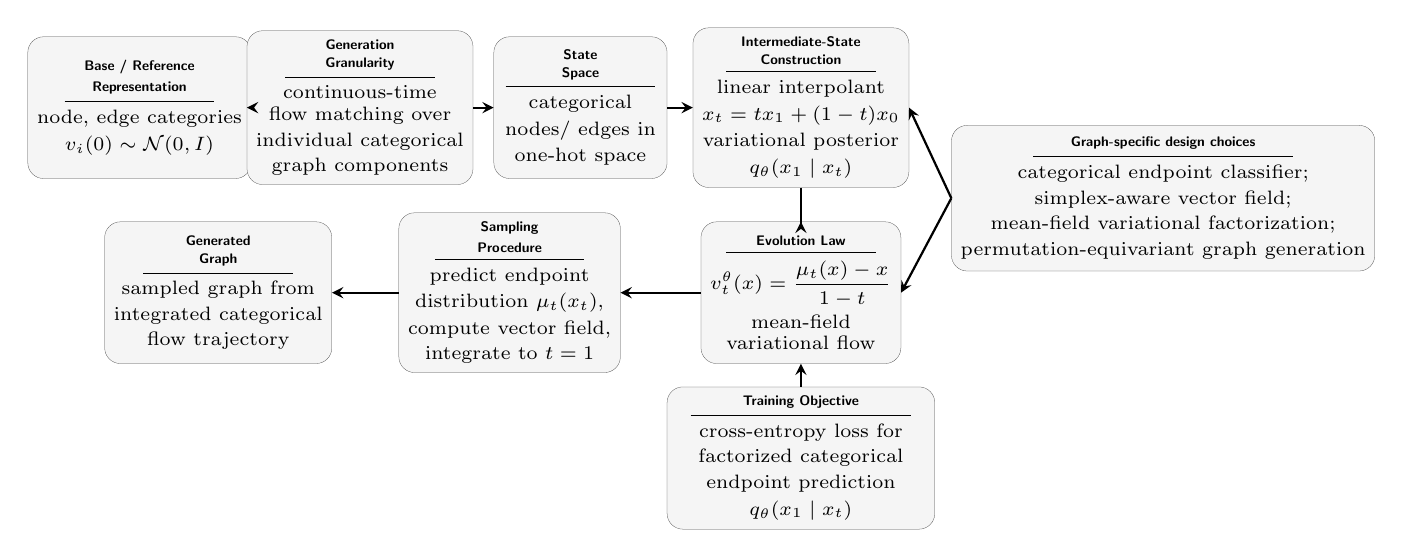
\begin{tikzpicture}[
    >=stealth,
    font=\scriptsize,
    box/.style={
        draw=black!70,
        rounded corners=2mm,
        ultra thin,
        minimum width=2.2cm,
        minimum height=1.8cm,
        align=center,
        fill=gray!8
    },
    side/.style={
        draw=black!70,
        rounded corners=2mm,
        ultra thin,
        minimum width=3.4cm,
        minimum height=1.45cm,
        align=center,
        fill=gray!8
    },
    note/.style={
        draw=black!70,
        rounded corners=2mm,
        ultra thin,
        minimum width=4.1cm,
        minimum height=1.85cm,
        align=center,
        fill=gray!8
    },
    arr/.style={->, thick}
]

\node[box] (base) at (0,0)
{\shortstack[c]{%
{\sffamily\bfseries\tiny Base / Reference}\\
{\sffamily\bfseries\tiny Representation}\\[-0.2mm]
\rule{1.9cm}{0.2pt}\\[0.0mm]
 node, edge categories \\ $v_i(0)\sim\mathcal N(0,I)$}};

\node[box] (time) at (2.8,0)
{\shortstack[c]{%
{\sffamily\bfseries\tiny Generation}\\
{\sffamily\bfseries\tiny Granularity}\\[-0.2mm]
\rule{1.9cm}{0.2pt}\\[0mm]
continuous-time\\
flow matching over\\
individual categorical\\
graph components}};

\node[box] (state) at (5.6,0)
{\shortstack[c]{%
{\sffamily\bfseries\tiny State}\\
{\sffamily\bfseries\tiny Space}\\[-0.2mm]
\rule{1.9cm}{0.2pt}\\[0mm]
categorical\\
nodes/ edges in\\
one-hot space}};

\node[box] (path) at (8.4,0)
{\shortstack[c]{%
{\sffamily\bfseries\tiny Intermediate-State}\\
{\sffamily\bfseries\tiny Construction}\\[-0.2mm]
\rule{1.9cm}{0.2pt}\\[0mm]
linear interpolant\\
$x_t=t x_1+(1-t)x_0$\\
variational posterior\\
$q_\theta(x_1\mid x_t)$}};

% second row
\node[box] (out) at (1.0,-2.35)
{\shortstack[c]{%
{\sffamily\bfseries\tiny Generated}\\
{\sffamily\bfseries\tiny Graph}\\[-0.2mm]
\rule{1.9cm}{0.2pt}\\[0mm]
sampled graph from\\
integrated categorical\\
flow trajectory}}; 

\node[box] (sample) at (4.7,-2.35)
{\shortstack[c]{%
{\sffamily\bfseries\tiny Sampling}\\
{\sffamily\bfseries\tiny Procedure}\\[-0.2mm]
\rule{1.9cm}{0.2pt}\\[0mm]
predict endpoint\\
distribution $\mu_t(x_t)$,\\
compute vector field,\\
integrate to $t=1$}};

\node[box] (evo) at (8.4,-2.35)
{\shortstack[c]{%
{\sffamily\bfseries\tiny Evolution Law}\\[-0.2mm]
\rule{1.9cm}{0.2pt}\\[0mm]
$v^\theta_t(x)=\dfrac{\mu_t(x)-x}{1-t}$\\
mean-field\\
variational flow}}; 

\draw[arr] (base) -- (time);
\draw[arr] (time) -- (state);
\draw[arr] (state) -- (path);
\draw[arr] (path.south) -- ++(0,-0.45) -| (evo.north);
\draw[arr] (evo) -- (sample);
\draw[arr] (sample) -- (out);

\node[side] (train) at (8.4,-4.45)
{\shortstack[c]{%
{\sffamily\bfseries\tiny Training Objective}\\[-0.2mm]
\rule{2.8cm}{0.2pt}\\[0mm]
cross-entropy loss for\\
factorized categorical\\
endpoint prediction\\
$ q_\theta(x_1 \mid x_t)$}};

\draw[arr] (train.north) -- (evo.south);

\node[note] (graphspec) at (13.0,-1.15)
{\shortstack[c]{%
{\sffamily\bfseries\tiny Graph-specific design choices}\\[-0.2mm]
\rule{3.3cm}{0.2pt}\\[0mm]
categorical endpoint classifier;\\
simplex-aware vector field;\\
mean-field variational factorization;\\
permutation-equivariant graph generation}}; 

\draw[arr] (graphspec.west) -- (path.east);
\draw[arr] (graphspec.west) -- (evo.east);

\end{tikzpicture}
\caption{CatFlow.}
\end{subfigure}

\vspace{0.8em}

% =========================
% Subfigure (b): GGFlow
% =========================
\begin{subfigure}[t]{\textwidth}
\centering
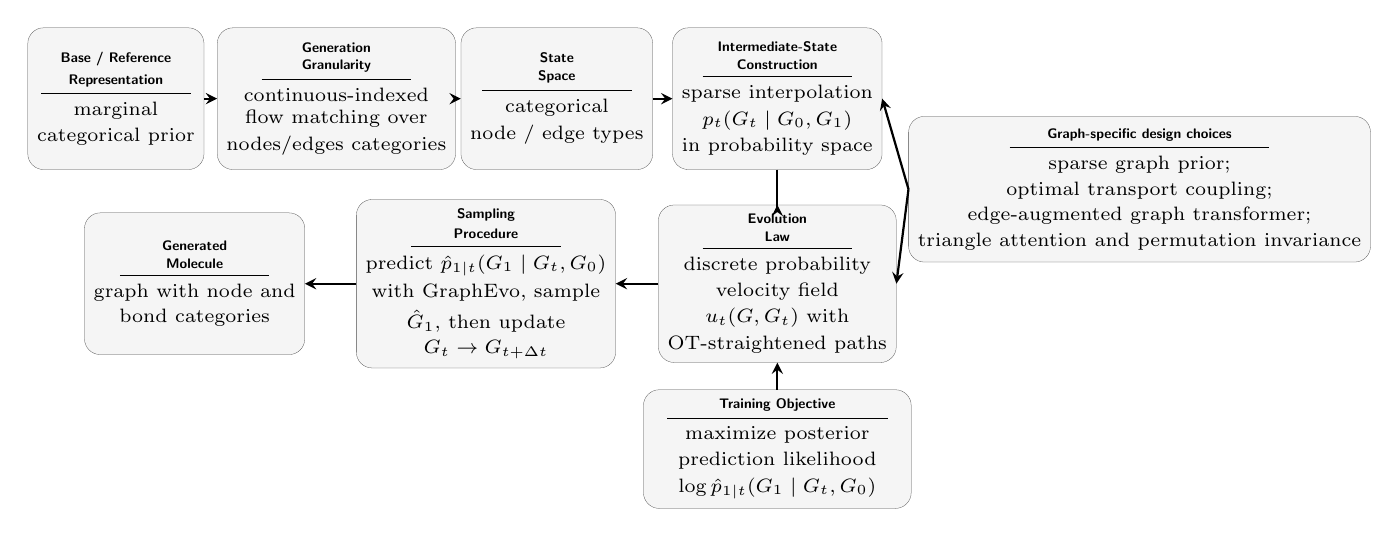
\begin{tikzpicture}[
    >=stealth,
    font=\scriptsize,
    box/.style={
        draw=black!70,
        rounded corners=2mm,
        ultra thin,
        minimum width=2.2cm,
        minimum height=1.8cm,
        align=center,
        fill=gray!8
    },
    side/.style={
        draw=black!70,
        rounded corners=2mm,
        ultra thin,
        minimum width=3.4cm,
        minimum height=1.45cm,
        align=center,
        fill=gray!8
    },
    note/.style={
        draw=black!70,
        rounded corners=2mm,
        ultra thin,
        minimum width=4.1cm,
        minimum height=1.85cm,
        align=center,
        fill=gray!8
    },
    arr/.style={->, thick}
]

\node[box] (base) at (0,0)
{\shortstack[c]{%
{\sffamily\bfseries\tiny Base / Reference}\\
{\sffamily\bfseries\tiny Representation}\\[-0.2mm]
\rule{1.9cm}{0.2pt}\\[0mm]
marginal\\ categorical prior}};

\node[box] (time) at (2.8,0)
{\shortstack[c]{%
{\sffamily\bfseries\tiny Generation}\\
{\sffamily\bfseries\tiny Granularity}\\[-0.2mm]
\rule{1.9cm}{0.2pt}\\[0mm]
continuous-indexed\\
flow matching over\\
nodes/edges categories}};

\node[box] (state) at (5.6,0)
{\shortstack[c]{%
{\sffamily\bfseries\tiny State}\\
{\sffamily\bfseries\tiny Space}\\[-0.2mm]
\rule{1.9cm}{0.2pt}\\[0mm]
categorical\\
node / edge types}}; 

\node[box] (path) at (8.4,0)
{\shortstack[c]{%
{\sffamily\bfseries\tiny Intermediate-State}\\
{\sffamily\bfseries\tiny Construction}\\[-0.2mm]
\rule{1.9cm}{0.2pt}\\[0mm]
sparse interpolation\\
$ p_t(G_t\mid G_0,G_1)$\\
in probability space}};

\node[box] (out) at (1.0,-2.35)
{\shortstack[c]{%
{\sffamily\bfseries\tiny Generated}\\
{\sffamily\bfseries\tiny Molecule}\\[-0.2mm]
\rule{1.9cm}{0.2pt}\\[0mm]
graph with node and\\
bond categories}}; 

\node[box] (sample) at (4.7,-2.35)
{\shortstack[c]{%
{\sffamily\bfseries\tiny Sampling}\\
{\sffamily\bfseries\tiny Procedure}\\[-0.2mm]
\rule{1.9cm}{0.2pt}\\[0mm]
predict $\hat p_{1\mid t}(G_1\mid G_t,G_0)$\\
with GraphEvo, sample\\
$\hat G_1$, then update\\
$G_t \rightarrow G_{t+\Delta t}$}}; 

\node[box] (evo) at (8.4,-2.35)
{\shortstack[c]{%
{\sffamily\bfseries\tiny Evolution}\\
{\sffamily\bfseries\tiny Law}\\[-0.2mm]
\rule{1.9cm}{0.2pt}\\[0mm]
discrete probability\\
velocity field\\
$u_t(G,G_t)$ with\\
OT-straightened paths}}; 

\draw[arr] (base) -- (time);
\draw[arr] (time) -- (state);
\draw[arr] (state) -- (path);
\draw[arr] (path.south) -- ++(0,-0.45) -| (evo.north);
\draw[arr] (evo) -- (sample);
\draw[arr] (sample) -- (out);

\node[side] (train) at (8.4,-4.45)
{\shortstack[c]{%
{\sffamily\bfseries\tiny Training Objective}\\[-0.2mm]
\rule{2.8cm}{0.2pt}\\[0mm]
maximize posterior\\
prediction likelihood\\
$\log \hat p_{1\mid t}(G_1\mid G_t,G_0)$}}; 

\draw[arr] (train.north) -- (evo.south);

\node[note] (graphspec) at (13.0,-1.15)
{\shortstack[c]{%
{\sffamily\bfseries\tiny Graph-specific design choices}\\[-0.2mm]
\rule{3.3cm}{0.2pt}\\[0mm]
sparse graph prior;\\
optimal transport coupling;\\
edge-augmented graph transformer;\\
triangle attention and permutation invariance}}; 

\draw[arr] (graphspec.west) -- (path.east);
\draw[arr] (graphspec.west) -- (evo.east);

\end{tikzpicture}
\caption{GGFlow.}
\end{subfigure}

\vspace{0.8em}

% =========================
% Subfigure (c): DeFoG
% =========================
\begin{subfigure}[t]{\textwidth}
\centering
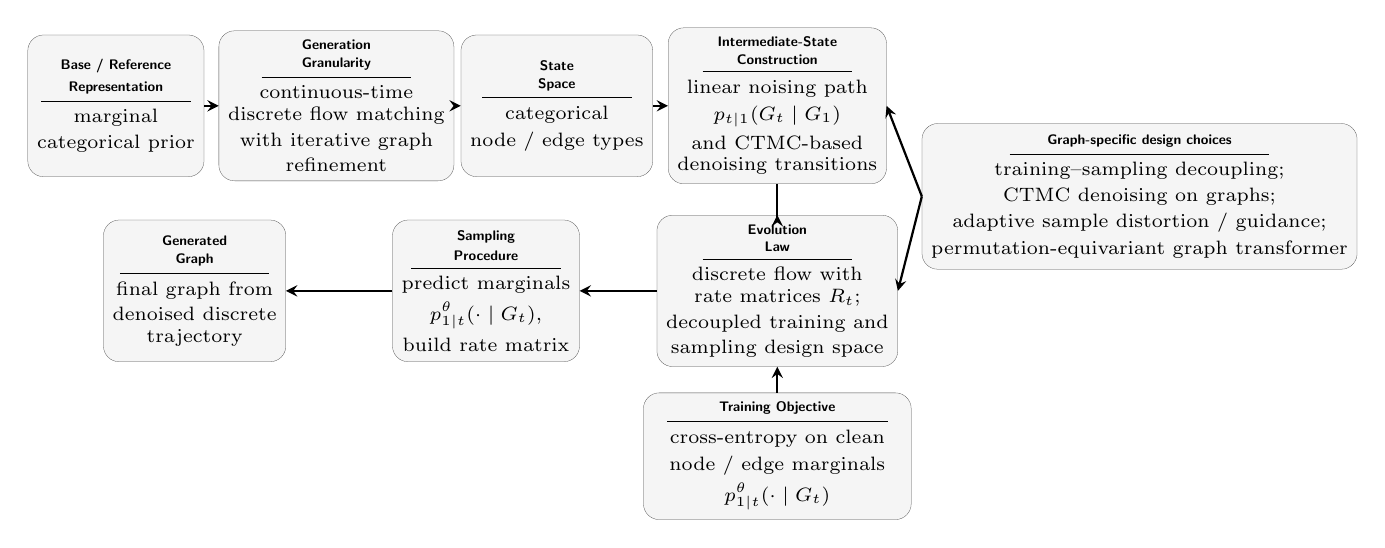
\begin{tikzpicture}[
    >=stealth,
    font=\scriptsize,
    box/.style={
        draw=black!70,
        rounded corners=2mm,
        ultra thin,
        minimum width=2.2cm,
        minimum height=1.8cm,
        align=center,
        fill=gray!8
    },
    side/.style={
        draw=black!70,
        rounded corners=2mm,
        ultra thin,
        minimum width=3.4cm,
        minimum height=1.45cm,
        align=center,
        fill=gray!8
    },
    note/.style={
        draw=black!70,
        rounded corners=2mm,
        ultra thin,
        minimum width=4.1cm,
        minimum height=1.85cm,
        align=center,
        fill=gray!8
    },
    arr/.style={->, thick}
]

\node[box] (base) at (0,0)
{\shortstack[c]{%
{\sffamily\bfseries\tiny Base / Reference}\\
{\sffamily\bfseries\tiny Representation}\\[-0.2mm]
\rule{1.9cm}{0.2pt}\\[0mm]
marginal\\ categorical prior}};

\node[box] (time) at (2.8,0)
{\shortstack[c]{%
{\sffamily\bfseries\tiny Generation}\\
{\sffamily\bfseries\tiny Granularity}\\[-0.2mm]
\rule{1.9cm}{0.2pt}\\[0mm]
continuous-time\\
discrete flow matching\\
with iterative graph\\
refinement}}; 

\node[box] (state) at (5.6,0)
{\shortstack[c]{%
{\sffamily\bfseries\tiny State}\\
{\sffamily\bfseries\tiny Space}\\[-0.2mm]
\rule{1.9cm}{0.2pt}\\[0mm]
categorical\\
node / edge types}}; 

\node[box] (path) at (8.4,0)
{\shortstack[c]{%
{\sffamily\bfseries\tiny Intermediate-State}\\
{\sffamily\bfseries\tiny Construction}\\[-0.2mm]
\rule{1.9cm}{0.2pt}\\[0mm]
linear noising path\\
$p_{t\mid 1}(G_t\mid G_1)$\\
and CTMC-based\\
denoising transitions}}; 

\node[box] (out) at (1.0,-2.35)
{\shortstack[c]{%
{\sffamily\bfseries\tiny Generated}\\
{\sffamily\bfseries\tiny Graph}\\[-0.2mm]
\rule{1.9cm}{0.2pt}\\[0mm]
final graph from\\
denoised discrete\\
trajectory}}; 

\node[box] (sample) at (4.7,-2.35)
{\shortstack[c]{%
{\sffamily\bfseries\tiny Sampling}\\
{\sffamily\bfseries\tiny Procedure}\\[-0.2mm]
\rule{1.9cm}{0.2pt}\\[0mm]
predict marginals\\
$p^\theta_{1\mid t}(\cdot\mid G_t)$,\\
build rate matrix}}; 

\node[box] (evo) at (8.4,-2.35)
{\shortstack[c]{%
{\sffamily\bfseries\tiny Evolution}\\
{\sffamily\bfseries\tiny Law}\\[-0.2mm]
\rule{1.9cm}{0.2pt}\\[0mm]
discrete flow with\\
rate matrices $R_t$;\\
decoupled training and\\
sampling design space}}; 

\draw[arr] (base) -- (time);
\draw[arr] (time) -- (state);
\draw[arr] (state) -- (path);
\draw[arr] (path.south) -- ++(0,-0.45) -| (evo.north);
\draw[arr] (evo) -- (sample);
\draw[arr] (sample) -- (out);

\node[side] (train) at (8.4,-4.45)
{\shortstack[c]{%
{\sffamily\bfseries\tiny Training Objective}\\[-0.2mm]
\rule{2.8cm}{0.2pt}\\[0mm]
cross-entropy on clean\\
node / edge marginals\\
$ p^\theta_{1\mid t}(\cdot\mid G_t)$}}; 

\draw[arr] (train.north) -- (evo.south);

\node[note] (graphspec) at (13.0,-1.15)
{\shortstack[c]{%
{\sffamily\bfseries\tiny Graph-specific design choices}\\[-0.2mm]
\rule{3.3cm}{0.2pt}\\[0mm]
training--sampling decoupling;\\
CTMC denoising on graphs;\\
adaptive sample distortion / guidance;\\
permutation-equivariant graph transformer}}; 

\draw[arr] (graphspec.west) -- (path.east);
\draw[arr] (graphspec.west) -- (evo.east);

\end{tikzpicture}
\caption{DeFoG.}
\end{subfigure}

\caption{Pipelines of three flow-based graph generators: CatFlow, GGFlow, and DeFoG.}
\label{fig:catflow_ggflow_defog_pipelines}
\end{figure*}
\emph{CatFlow} \cite{eijkelboom2024vfm} belongs to \emph{flow matching / conditional flow matching} within the broader family of \emph{ODE-based deterministic models}. It generates graphs in a \emph{relaxed graph space}, where categorical node and edge variables are transported continuously from a simple base distribution, typically a standard Gaussian, to the data distribution along a linear interpolation path $x_t = tx_1 +(1-t)x_0$. The flow is driven by a learned velocity field induced from a factorized variational posterior over endpoints, and training uses a \emph{variational flow-matching objective} that reduces to a \emph{cross-entropy loss} over endpoint classes in the categorical setting. Sampling then proceeds by \emph{ODE integration}, with graph-specific design choices including permutation-equivariant modeling, continuous transport of categorical node-edge attributes, and trajectories biased toward the probability simplex for more structured generation.


\emph{GGFlow} \cite{hou2024ggflow} is a \emph{discrete-state continuous-time flow-matching} model for graph generation. It evolves in \emph{discrete graph space}, with categorical node and edge attributes throughout, starting from a sparsity-aware \emph{factorized categorical prior} over nodes and edges. Intermediate states are constructed by a \emph{prescribed conditional interpolation path} that samples each node and edge variable from a time-dependent categorical mixture of the source and target graphs. The dynamics are governed by a learned \emph{conditional transition-rate field}, approximated by GraphEvo via terminal-graph posterior prediction and trained with a \emph{cross-entropy-style variational objective}. Its main graph-specific choices are sparsity-preserving priors, permutation-aware design through invariant priors and OT coupling, and edge-augmented graph transformers that improve structural modeling and sampling efficiency.

\emph{DeFoG} \cite{qin2025defog} is best placed under \emph{flow matching and conditional flow matching}, more specifically as a \emph{discrete flow-matching} method whose reverse process is implemented as a CTMC. It operates in \emph{discrete graph space}, keeping node and edge variables categorical throughout generation, and starts from a simple factorized base distribution over node and edge categories. Intermediate states follow a \emph{prescribed linear interpolation path} between the clean graph and the base distribution, while the reverse dynamics are defined by a learned \emph{transition-rate function} constructed from predicted clean node and edge marginals. Training uses a \emph{cross-entropy denoising objective} to predict clean node and edge states from a noisy graph at arbitrary time t, and sampling proceeds by CTMC-style jump simulation with Euler steps. Its main graph-specific features are permutation-equivariant denoising, direct discrete node-edge modeling, and flexible sampling through the decoupling of training and sampling, which enables time distortion, target guidance, and stochasticity control without retraining.


\emph{Evaluation .} CatFlow, GGFlow, and DeFoG all show that discrete flow-based graph generators can achieve strong empirical performance by modeling node and edge distributions directly, often improving sample quality, efficiency, and permutation handling relative to simpler baselines or continuous relaxations. At the same time, like most deep graph generators, they still capture many higher-order dependencies, implicit global properties, and large combinatorial output spaces only approximately through learned denoising, interpolation, or jump dynamics, so important structural qualities are often assessed indirectly through benchmark statistics rather than enforced explicitly. As a result, validity can be strong in practice, especially for molecular and benchmark graph generation, but hard constraints such as connectivity, acyclicity, or full domain correctness are generally not guaranteed by construction; and although these models are somewhat more structured and tunable than many alternatives because they predict endpoint distributions and derive dynamics from them, they remain largely neural black boxes whose behavior is still difficult to fully interpret, verify, and reliably control in constraint-sensitive settings.


\begin{figure*}[htbp]
\centering


\vspace{0.8em}

% =========================
% Subfigure (b): BWFlow
% =========================
\begin{subfigure}[t]{\textwidth}
\centering
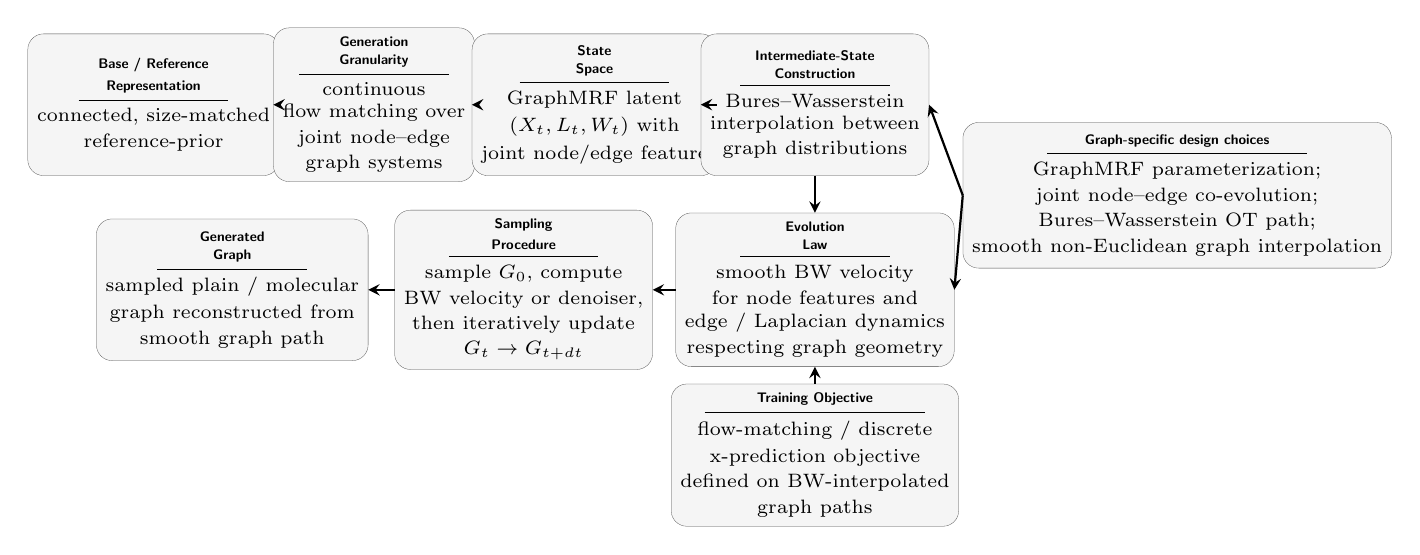
\begin{tikzpicture}[
    >=stealth,
    font=\scriptsize,
    box/.style={
        draw=black!70,
        rounded corners=2mm,
        ultra thin,
        minimum width=2.2cm,
        minimum height=1.8cm,
        align=center,
        fill=gray!8
    },
    side/.style={
        draw=black!70,
        rounded corners=2mm,
        ultra thin,
        minimum width=3.4cm,
        minimum height=1.45cm,
        align=center,
        fill=gray!8
    },
    note/.style={
        draw=black!70,
        rounded corners=2mm,
        ultra thin,
        minimum width=4.1cm,
        minimum height=1.85cm,
        align=center,
        fill=gray!8
    },
    arr/.style={->, thick}
]

\node[box] (base) at (0,0)
{\shortstack[c]{%
{\sffamily\bfseries\tiny Base / Reference}\\
{\sffamily\bfseries\tiny Representation}\\[-0.2mm]
\rule{1.9cm}{0.2pt}\\[0mm]
connected, size-matched\\
reference-prior}}; 

\node[box] (time) at (2.8,0)
{\shortstack[c]{%
{\sffamily\bfseries\tiny Generation}\\
{\sffamily\bfseries\tiny Granularity}\\[-0.2mm]
\rule{1.9cm}{0.2pt}\\[0mm]
continuous\\
flow matching over\\
joint node--edge\\
graph systems}}; 

\node[box] (state) at (5.6,0)
{\shortstack[c]{%
{\sffamily\bfseries\tiny State}\\
{\sffamily\bfseries\tiny Space}\\[-0.2mm]
\rule{1.9cm}{0.2pt}\\[0mm]
GraphMRF latent\\
$(X_t,L_t,W_t)$ with\\
joint node/edge feature}}; 

\node[box] (path) at (8.4,0)
{\shortstack[c]{%
{\sffamily\bfseries\tiny Intermediate-State}\\
{\sffamily\bfseries\tiny Construction}\\[-0.2mm]
\rule{1.9cm}{0.2pt}\\[0mm]
Bures--Wasserstein\\
interpolation between\\
graph distributions}}; 

\node[box] (out) at (1.0,-2.35)
{\shortstack[c]{%
{\sffamily\bfseries\tiny Generated}\\
{\sffamily\bfseries\tiny Graph}\\[-0.2mm]
\rule{1.9cm}{0.2pt}\\[0mm]
sampled plain / molecular\\
graph reconstructed from\\
smooth graph path}}; 

\node[box] (sample) at (4.7,-2.35)
{\shortstack[c]{%
{\sffamily\bfseries\tiny Sampling}\\
{\sffamily\bfseries\tiny Procedure}\\[-0.2mm]
\rule{1.9cm}{0.2pt}\\[0mm]
sample $G_0$, compute\\
BW velocity or denoiser,\\
then iteratively update\\
$G_t \rightarrow G_{t+dt}$}}; 

\node[box] (evo) at (8.4,-2.35)
{\shortstack[c]{%
{\sffamily\bfseries\tiny Evolution}\\
{\sffamily\bfseries\tiny Law}\\[-0.2mm]
\rule{1.9cm}{0.2pt}\\[0mm]
smooth BW velocity\\
for node features and\\
edge / Laplacian dynamics\\
respecting graph geometry}}; 

\draw[arr] (base) -- (time);
\draw[arr] (time) -- (state);
\draw[arr] (state) -- (path);
\draw[arr] (path.south) -- ++(0,-0.45) -| (evo.north);
\draw[arr] (evo) -- (sample);
\draw[arr] (sample) -- (out);

\node[side] (train) at (8.4,-4.45)
{\shortstack[c]{%
{\sffamily\bfseries\tiny Training Objective}\\[-0.2mm]
\rule{2.8cm}{0.2pt}\\[0mm]
flow-matching / discrete\\
x-prediction objective\\
defined on BW-interpolated\\
graph paths}}; 

\draw[arr] (train.north) -- (evo.south);

\node[note] (graphspec) at (13.0,-1.15)
{\shortstack[c]{%
{\sffamily\bfseries\tiny Graph-specific design choices}\\[-0.2mm]
\rule{3.3cm}{0.2pt}\\[0mm]
GraphMRF parameterization;\\
joint node--edge co-evolution;\\
Bures--Wasserstein OT path;\\
smooth non-Euclidean graph interpolation}}; 

\draw[arr] (graphspec.west) -- (path.east);
\draw[arr] (graphspec.west) -- (evo.east);

\end{tikzpicture}
\caption{BWFlow.}
\end{subfigure}

\vspace{0.8em}

% =========================
% Subfigure (c): GGBall
% =========================
\begin{subfigure}[t]{\textwidth}
\centering
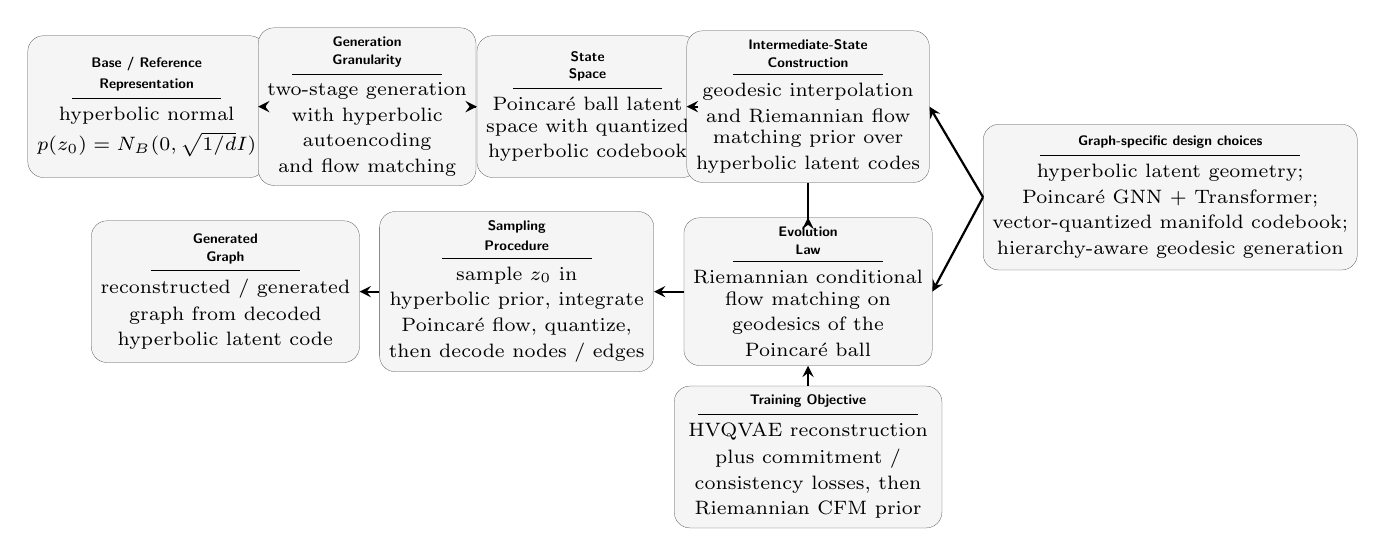
\begin{tikzpicture}[
    >=stealth,
    font=\scriptsize,
    box/.style={
        draw=black!70,
        rounded corners=2mm,
        ultra thin,
        minimum width=2.2cm,
        minimum height=1.8cm,
        align=center,
        fill=gray!8
    },
    side/.style={
        draw=black!70,
        rounded corners=2mm,
        ultra thin,
        minimum width=3.4cm,
        minimum height=1.45cm,
        align=center,
        fill=gray!8
    },
    note/.style={
        draw=black!70,
        rounded corners=2mm,
        ultra thin,
        minimum width=4.1cm,
        minimum height=1.85cm,
        align=center,
        fill=gray!8
    },
    arr/.style={->, thick}
]

\node[box] (base) at (0,0)
{\shortstack[c]{%
{\sffamily\bfseries\tiny Base / Reference}\\
{\sffamily\bfseries\tiny Representation}\\[-0.2mm]
\rule{1.9cm}{0.2pt}\\[0mm]
hyperbolic normal\\
$p(z_0)=N_B(0,\sqrt{1/d}I)$}}; 

\node[box] (time) at (2.8,0)
{\shortstack[c]{%
{\sffamily\bfseries\tiny Generation}\\
{\sffamily\bfseries\tiny Granularity}\\[-0.2mm]
\rule{1.9cm}{0.2pt}\\[0mm]
two-stage generation\\
with hyperbolic\\
 autoencoding\\
and flow matching}}; 

\node[box] (state) at (5.6,0)
{\shortstack[c]{%
{\sffamily\bfseries\tiny State}\\
{\sffamily\bfseries\tiny Space}\\[-0.2mm]
\rule{1.9cm}{0.2pt}\\[0mm]
Poincaré ball latent\\
space with quantized\\
hyperbolic codebook}}; 

\node[box] (path) at (8.4,0)
{\shortstack[c]{%
{\sffamily\bfseries\tiny Intermediate-State}\\
{\sffamily\bfseries\tiny Construction}\\[-0.2mm]
\rule{1.9cm}{0.2pt}\\[0mm]
geodesic interpolation\\
and Riemannian flow\\
matching prior over\\
hyperbolic latent codes}}; 

\node[box] (out) at (1.0,-2.35)
{\shortstack[c]{%
{\sffamily\bfseries\tiny Generated}\\
{\sffamily\bfseries\tiny Graph}\\[-0.2mm]
\rule{1.9cm}{0.2pt}\\[0mm]
reconstructed / generated\\
graph from decoded\\
hyperbolic latent code}}; 

\node[box] (sample) at (4.7,-2.35)
{\shortstack[c]{%
{\sffamily\bfseries\tiny Sampling}\\
{\sffamily\bfseries\tiny Procedure}\\[-0.2mm]
\rule{1.9cm}{0.2pt}\\[0mm]
sample $z_0$ in\\
hyperbolic prior, integrate\\
Poincaré flow, quantize,\\
then decode nodes / edges}}; 

\node[box] (evo) at (8.4,-2.35)
{\shortstack[c]{%
{\sffamily\bfseries\tiny Evolution}\\
{\sffamily\bfseries\tiny Law}\\[-0.2mm]
\rule{1.9cm}{0.2pt}\\[0mm]
Riemannian conditional\\
flow matching on\\
geodesics of the\\
Poincaré ball}}; 

\draw[arr] (base) -- (time);
\draw[arr] (time) -- (state);
\draw[arr] (state) -- (path);
\draw[arr] (path.south) -- ++(0,-0.45) -| (evo.north);
\draw[arr] (evo) -- (sample);
\draw[arr] (sample) -- (out);

\node[side] (train) at (8.4,-4.45)
{\shortstack[c]{%
{\sffamily\bfseries\tiny Training Objective}\\[-0.2mm]
\rule{2.8cm}{0.2pt}\\[0mm]
HVQVAE reconstruction\\
plus commitment /\\
consistency losses, then\\
Riemannian CFM prior}}; 

\draw[arr] (train.north) -- (evo.south);

\node[note] (graphspec) at (13.0,-1.15)
{\shortstack[c]{%
{\sffamily\bfseries\tiny Graph-specific design choices}\\[-0.2mm]
\rule{3.3cm}{0.2pt}\\[0mm]
hyperbolic latent geometry;\\
Poincaré GNN + Transformer;\\
vector-quantized manifold codebook;\\
hierarchy-aware geodesic generation}}; 

\draw[arr] (graphspec.west) -- (path.east);
\draw[arr] (graphspec.west) -- (evo.east);

\end{tikzpicture}
\caption{GGBall.}
\end{subfigure}

\caption{Pipelines of two transport-based / geometry-aware generative models: BWFlow, and GGBall.}
\label{fig:alignflow_bwflow_ggball_pipelines}
\end{figure*}


\paragraph{Rectified flow.}
Rectified-flow-style methods can be viewed as a special case of flow matching in which the transport path is chosen to be especially simple, often close to a straight interpolation, so that learning and sampling become easier. In graph generation, this viewpoint is most natural when graphs are embedded in continuous latent spaces or continuous relaxations where low-curvature paths can be defined explicitly. Since the current representative graph literature in this subsection is already well covered by the broader flow-matching and geometry-aware transport viewpoints, we treat rectified flow here primarily as a conceptual simplification rather than as a separate major branch.

\paragraph{Geometry-aware transport and interpolants.}
A major recent direction in continuous-time graph generation is to replace naive Euclidean interpolation with geometry-aware transport paths that better respect the structure of graph representations. These approaches are motivated by the observation that the quality of continuous-time transport depends not only on the learned dynamics but also on the geometry of the interpolation path, the endpoint coupling, and the representation space in which transport is performed.


\emph{BWFlow} \cite{bwflow} is best placed among \emph{geometry-aware transport models} within the broader class of \emph{ODE-based deterministic generators}. It uses \emph{flow matching} on a \emph{Bures--Wasserstein interpolation path} defined over a GraphMRF-based relaxed graph space, with an additional discrete variant for categorical nodes and Bernoulli edges. Starting from a \emph{reference graph distribution}, it transports samples toward the data distribution through a closed-form interpolation that jointly models node and edge evolution. The dynamics are learned through a \emph{velocity field}, or equivalently an \emph{$x$-prediction objective}, and sampling follows \emph{ODE integration}. Its key graph-specific feature is a geometry-aware transport path that better preserves structural coherence than independent Euclidean interpolation.

\emph{GGBall} \cite{ggball} is a \emph{geometry-aware transport model} in the class of \emph{ODE-based deterministic generators}. It performs graph generation in a \emph{hyperbolic latent space} on the Poincar'e ball, starting from a \emph{hyperbolic base distribution} and transporting samples to graph latents along \emph{geodesic interpolation paths}. The dynamics are governed by a learned manifold-valued \emph{velocity field}, trained with \emph{Riemannian conditional flow matching}, and sampling is performed by \emph{ODE integration}, followed by \emph{vector quantization and decoding} into node and edge attributes. Its graph-specific design emphasizes \emph{hierarchy-aware hyperbolic representations}, discrete graph reconstruction through latent decoding, and the use of \emph{curvature-aware geometry} to better capture tree-like and modular structures.


\emph{Evaluation.} BWFlow and GGBall both strengthen graph generation by imposing a more structured geometric transport process than naïve interpolation-based models, but they do so in different spaces and with different inductive biases. BWFlow models joint node--edge evolution directly through a GraphMRF representation and Bures--Wasserstein interpolation, giving it a principled treatment of graph dependencies and a more interpretable transport path than many heuristic flow models, while GGBall instead mitigates the difficulty of large combinatorial graph spaces by moving generation into a hyperbolic latent space, where geometry-aware encoding, geodesic transport, and latent decoding better capture hierarchical, modular, and tree-like structure. In both cases, however, permutation ambiguity is only handled indirectly rather than resolved explicitly, and many higher-order or implicit global properties are still assessed mainly through benchmark statistics instead of being guaranteed by design. Likewise, both methods only partially address validity: BWFlow does not enforce hard structural constraints such as connectivity, acyclicity, or full chemical correctness, and GGBall, despite improving reconstruction quality and empirical molecular validity through its hyperbolic autoencoding and decoding pipeline, also lacks such guarantees by construction. More broadly, although BWFlow is somewhat more interpretable because its velocity field is tied to an explicit probabilistic geometry, and GGBall benefits from the clearer inductive bias of the Poincaré ball, both remain largely neural black-box generators whose behavior can still be difficult to diagnose, control, or trust in reliability-critical and constraint-sensitive settings.

\subsection{SDE-Based Diffusion and Score Models}
\label{sec:sde_models}

SDE-based diffusion and score models define graph generation through a stochastic continuous-time evolution in which data are gradually perturbed by a forward process and recovered by learned reverse-time dynamics. In graph settings, these methods are typically implemented in continuous relaxations of adjacency and feature variables, belief-space parameterizations, or score-based stochastic refinement frameworks rather than directly on discrete combinatorial graph states. The key design choices concern the noise process, the learned score or denoiser, and which graph symmetry and validity are preserved during sampling.


\begin{figure*}[htbp]
\centering

% =========================
% Subfigure (a): PRODIGY
% =========================
\begin{subfigure}[t]{\textwidth}
\centering
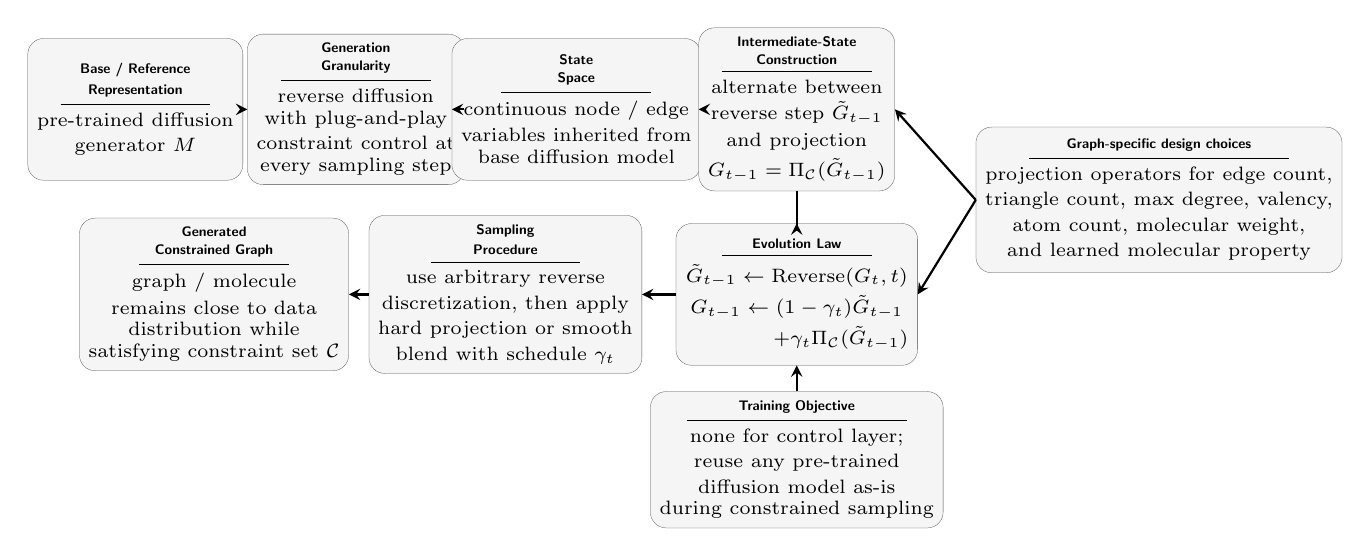
\begin{tikzpicture}[
    >=stealth,
    font=\scriptsize,
    box/.style={
        draw=black!70,
        rounded corners=2mm,
        ultra thin,
        minimum width=2.2cm,
        minimum height=1.8cm,
        align=center,
        fill=gray!8
    },
    side/.style={
        draw=black!70,
        rounded corners=2mm,
        ultra thin,
        minimum width=3.4cm,
        minimum height=1.45cm,
        align=center,
        fill=gray!8
    },
    note/.style={
        draw=black!70,
        rounded corners=2mm,
        ultra thin,
        minimum width=4.1cm,
        minimum height=1.85cm,
        align=center,
        fill=gray!8
    },
    arr/.style={->, thick}
]

\node[box] (base) at (0,0)
{\shortstack[c]{%
{\sffamily\bfseries\tiny Base / Reference}\\
{\sffamily\bfseries\tiny Representation}\\[-0.2mm]
\rule{1.9cm}{0.2pt}\\[0mm]
pre-trained diffusion\\
generator $M$}};

\node[box] (time) at (2.8,0)
{\shortstack[c]{%
{\sffamily\bfseries\tiny Generation}\\
{\sffamily\bfseries\tiny Granularity}\\[-0.2mm]
\rule{1.9cm}{0.2pt}\\[0mm]
reverse diffusion\\
with plug-and-play\\
constraint control at\\
every sampling step}};

\node[box] (state) at (5.6,0)
{\shortstack[c]{%
{\sffamily\bfseries\tiny State}\\
{\sffamily\bfseries\tiny Space}\\[-0.2mm]
\rule{1.9cm}{0.2pt}\\[0mm]
continuous node / edge\\
variables inherited from\\
base diffusion model}};

\node[box] (path) at (8.4,0)
{\shortstack[c]{%
{\sffamily\bfseries\tiny Intermediate-State}\\
{\sffamily\bfseries\tiny Construction}\\[-0.2mm]
\rule{1.9cm}{0.2pt}\\[0mm]
alternate between\\
reverse step $\tilde G_{t-1}$\\
and projection\\
$G_{t-1}=\Pi_{\mathcal C}(\tilde G_{t-1})$}};

\node[box] (out) at (1.0,-2.35)
{\shortstack[c]{%
{\sffamily\bfseries\tiny Generated}\\
{\sffamily\bfseries\tiny Constrained Graph}\\[-0.2mm]
\rule{1.9cm}{0.2pt}\\[0mm]
graph / molecule \\
remains close to data\\
distribution while\\
satisfying constraint set $\mathcal C$}}; 

\node[box] (sample) at (4.7,-2.35)
{\shortstack[c]{%
{\sffamily\bfseries\tiny Sampling}\\
{\sffamily\bfseries\tiny Procedure}\\[-0.2mm]
\rule{1.9cm}{0.2pt}\\[0mm]
use arbitrary reverse\\
discretization, then apply\\
hard projection or smooth\\
blend with schedule $\gamma_t$}}; 

\node[box] (evo) at (8.4,-2.35)
{\shortstack[c]{%
{\sffamily\bfseries\tiny Evolution Law}\\[-0.2mm]
\rule{1.9cm}{0.2pt}\\[0mm]
$\tilde G_{t-1}\leftarrow\mathrm{Reverse}(G_t,t)$\\
$G_{t-1}\leftarrow(1-\gamma_t)\tilde G_{t-1}$\\
$\qquad\qquad + \gamma_t\Pi_{\mathcal C}(\tilde G_{t-1})$}}; 

\draw[arr] (base) -- (time);
\draw[arr] (time) -- (state);
\draw[arr] (state) -- (path);
\draw[arr] (path.south) -- ++(0,-0.45) -| (evo.north);
\draw[arr] (evo) -- (sample);
\draw[arr] (sample) -- (out);

\node[side] (train) at (8.4,-4.45)
{\shortstack[c]{%
{\sffamily\bfseries\tiny Training Objective}\\[-0.2mm]
\rule{2.8cm}{0.2pt}\\[0mm]
none for control layer;\\
reuse any pre-trained\\
diffusion model as-is\\
during constrained sampling}}; 

\draw[arr] (train.north) -- (evo.south);

\node[note] (graphspec) at (13.0,-1.15)
{\shortstack[c]{%
{\sffamily\bfseries\tiny Graph-specific design choices}\\[-0.2mm]
\rule{3.3cm}{0.2pt}\\[0mm]
projection operators for edge count,\\
triangle count, max degree, valency,\\
atom count, molecular weight,\\
and learned molecular property}}; 

\draw[arr] (graphspec.west) -- (path.east);
\draw[arr] (graphspec.west) -- (evo.east);

\end{tikzpicture}
\caption{PRODIGY.}
\end{subfigure}

\vspace{0.8em}

% =========================
% Subfigure (b): GraphBSI
% =========================
\begin{subfigure}[t]{\textwidth}
\centering
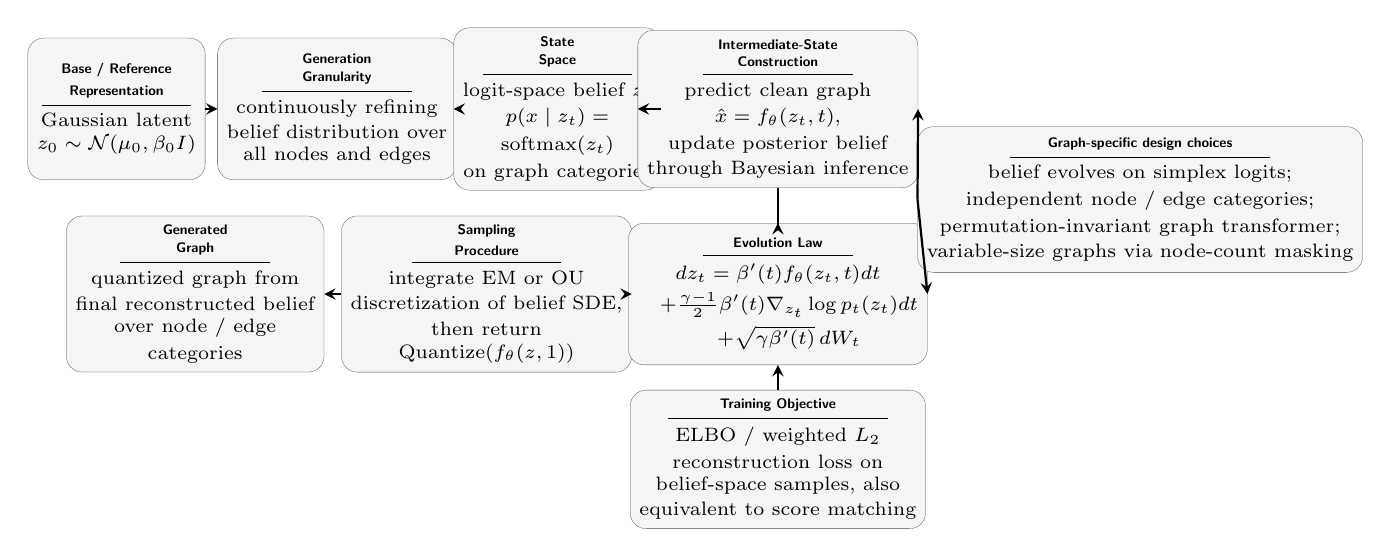
\begin{tikzpicture}[
    >=stealth,
    font=\scriptsize,
    box/.style={
        draw=black!70,
        rounded corners=2mm,
        ultra thin,
        minimum width=2.2cm,
        minimum height=1.8cm,
        align=center,
        fill=gray!8
    },
    side/.style={
        draw=black!70,
        rounded corners=2mm,
        ultra thin,
        minimum width=3.4cm,
        minimum height=1.45cm,
        align=center,
        fill=gray!8
    },
    note/.style={
        draw=black!70,
        rounded corners=2mm,
        ultra thin,
        minimum width=4.1cm,
        minimum height=1.85cm,
        align=center,
        fill=gray!8
    },
    arr/.style={->, thick}
]

\node[box] (base) at (0,0)
{\shortstack[c]{%
{\sffamily\bfseries\tiny Base / Reference}\\
{\sffamily\bfseries\tiny Representation}\\[-0.2mm]
\rule{1.9cm}{0.2pt}\\[0mm]
Gaussian latent\\
$z_0 \sim \mathcal N(\mu_0,\beta_0 I)$}}; 

\node[box] (time) at (2.8,0)
{\shortstack[c]{%
{\sffamily\bfseries\tiny Generation}\\
{\sffamily\bfseries\tiny Granularity}\\[-0.2mm]
\rule{1.9cm}{0.2pt}\\[0mm]
continuously refining\\
belief distribution over\\
all nodes and edges}}; 

\node[box] (state) at (5.6,0)
{\shortstack[c]{%
{\sffamily\bfseries\tiny State}\\
{\sffamily\bfseries\tiny Space}\\[-0.2mm]
\rule{1.9cm}{0.2pt}\\[0mm]
logit-space belief $z_t$\\
$p(x\mid z_t)=$\\$\mathrm{softmax}(z_t)$\\
on graph categories}}; 

\node[box] (path) at (8.4,0)
{\shortstack[c]{%
{\sffamily\bfseries\tiny Intermediate-State}\\
{\sffamily\bfseries\tiny Construction}\\[-0.2mm]
\rule{1.9cm}{0.2pt}\\[0mm]
predict clean graph\\
$\hat x=f_\theta(z_t,t)$,\\
update posterior belief\\
through Bayesian inference}}; 

\node[box] (out) at (1.0,-2.35)
{\shortstack[c]{%
{\sffamily\bfseries\tiny Generated}\\
{\sffamily\bfseries\tiny Graph}\\[-0.2mm]
\rule{1.9cm}{0.2pt}\\[0mm]
quantized graph from\\
final reconstructed belief\\
over node / edge\\
categories}}; 

\node[box] (sample) at (4.7,-2.35)
{\shortstack[c]{%
{\sffamily\bfseries\tiny Sampling}\\
{\sffamily\bfseries\tiny Procedure}\\[-0.2mm]
\rule{1.9cm}{0.2pt}\\[0mm]
integrate EM or OU\\
discretization of belief SDE,\\
then return\\
$\mathrm{Quantize}(f_\theta(z,1))$}}; 

\node[box] (evo) at (8.4,-2.35)
{\shortstack[c]{%
{\sffamily\bfseries\tiny Evolution Law}\\[-0.2mm]
\rule{1.9cm}{0.2pt}\\[0mm]
$d z_t = \beta'(t)f_\theta(z_t,t)dt$\\
$\quad + \frac{\gamma-1}{2}\beta'(t)\nabla_{z_t}\log p_t(z_t)dt$\\
$\quad + \sqrt{\gamma\beta'(t)}\,dW_t$}}; 

\draw[arr] (base) -- (time);
\draw[arr] (time) -- (state);
\draw[arr] (state) -- (path);
\draw[arr] (path.south) -- ++(0,-0.45) -| (evo.north);
\draw[arr] (evo) -- (sample);
\draw[arr] (sample) -- (out);

\node[side] (train) at (8.4,-4.45)
{\shortstack[c]{%
{\sffamily\bfseries\tiny Training Objective}\\[-0.2mm]
\rule{2.8cm}{0.2pt}\\[0mm]
ELBO / weighted $L_2$\\
reconstruction loss on\\
belief-space samples, also\\
equivalent to score matching}}; 

\draw[arr] (train.north) -- (evo.south);

\node[note] (graphspec) at (13.0,-1.15)
{\shortstack[c]{%
{\sffamily\bfseries\tiny Graph-specific design choices}\\[-0.2mm]
\rule{3.3cm}{0.2pt}\\[0mm]
belief evolves on simplex logits;\\
independent node / edge categories;\\
permutation-invariant graph transformer;\\
variable-size graphs via node-count masking}}; 

\draw[arr] (graphspec.west) -- (path.east);
\draw[arr] (graphspec.west) -- (evo.east);

\end{tikzpicture}
\caption{GraphBSI.}
\end{subfigure}

\caption{Pipelines of PRODIGY and GraphBSI. Top: PRODIGY adds projection-based controllable sampling on top of a pre-trained diffusion graph generator. Bottom: GraphBSI performs graph generation by refining a continuous belief over discrete node and edge categories through Bayesian sample inference and SDE-based sampling.}
\label{fig:prodigy_graphbsi_pipelines}
\end{figure*}


\emph{PRODIGY} \cite{sharma2024plug} belongs to the \emph{SDE-based diffusion and score} class because it operates by modifying the \emph{reverse-time stochastic sampling dynamics} of a pre-trained graph diffusion model with projection-based constraint enforcement. Its state space is a \emph{relaxed graph space}, where node features and adjacency variables remain continuous during sampling and are discretized only at the end. It inherits its \emph{base distribution}, forward noising process, and reverse drift--diffusion dynamics from the underlying diffusion model, while adding a \emph{projection operator} after each reverse step, or a smoothed variant of it, to move samples toward a user-specified constraint set. PRODIGY introduces \emph{no new training objective}, since it is purely a plug-and-play sampling method; its controllable component instead relies on analytically derived projectors for constraints such as edge count, degree, valency, atom count, molecular weight, and molecular properties. Its main graph-specific contributions are \emph{explicit constraint enforcement during sampling}, \emph{continuous-to-discrete graph generation}, and \emph{plug-and-play controllability without retraining}


\emph{GraphBSI} \cite{song2025smooth} is best placed under \emph{SDE-based diffusion and score models} within \emph{continuous-time graph generation}. It generates graphs through a \emph{continuous-time stochastic evolution in belief space}, where the latent state represents a distribution over node and edge categories rather than a discrete graph itself. Its state space is therefore a \emph{continuous parameter space of categorical beliefs}, initialized from a \emph{Gaussian prior} over logits. Intermediate states arise from \emph{iterative Bayesian updates} in this latent space, which converge in the infinitesimal-step limit to an \emph{SDE}. The evolution law is a \emph{drift--diffusion process} on the logits, with a noise-controlled family of samplers spanning deterministic probability-flow ODEs to more stochastic samplers. Training uses an \emph{ELBO-derived reconstruction objective}, shown to be equivalent to a weighted score-matching loss under a suitable parameterization. Sampling proceeds by \emph{SDE simulation} in belief space, using either Euler--Maruyama or Ornstein--Uhlenbeck discretization, followed by \emph{quantization} into a discrete graph. Its main graph-specific design choices are \emph{permutation invariance}, \emph{variable-size graph generation via node-count sampling and masking}, and a \emph{continuous-to-discrete formulation} that evolves logits over categorical graph variables rather than graph states directly.


\emph{Evaluation .} PRODIGY and GraphBSI address graph generation challenges from different angles. PRODIGY is strongest on validity requirements and partially on implicit properties, since it can explicitly enforce user-specified structural or molecular constraints during sampling, but it largely inherits its handling of non-unique representations, complex dependencies, and large output spaces from the underlying diffusion backbone, while the overall generator remains only partly more reliable than a standard black-box sampler. By contrast, GraphBSI better accommodates non-unique representations and large output spaces by evolving continuous permutation-invariant beliefs over categorical graph variables rather than discrete construction orders, but it models complex dependencies, implicit global properties, and validity requirements mainly through a learned reconstructor rather than explicit structural enforcement. As a result, PRODIGY offers stronger controllability and constraint satisfaction, whereas GraphBSI offers a smoother and more principled latent-space generation process, though both still retain substantial neural black-box behavior.

\subsection{CTMC and Discrete-State Continuous-Time Models}
\label{sec:ctmc_models}

CTMC-based models provide a continuous-time formulation that acts directly on discrete graph variables through jump processes rather than continuous trajectories. This family is especially appealing for graph generation because it avoids the mismatch introduced by continuous relaxations and preserves the discrete nature of node and edge states throughout generation. The main design questions concern the choice of rate parameterization, the tractability of reverse-time simulation, and the incorporation of graph-specific structure such as sparsity, permutation symmetry, and categorical constraints.

\begin{figure*}[htbp]
\centering

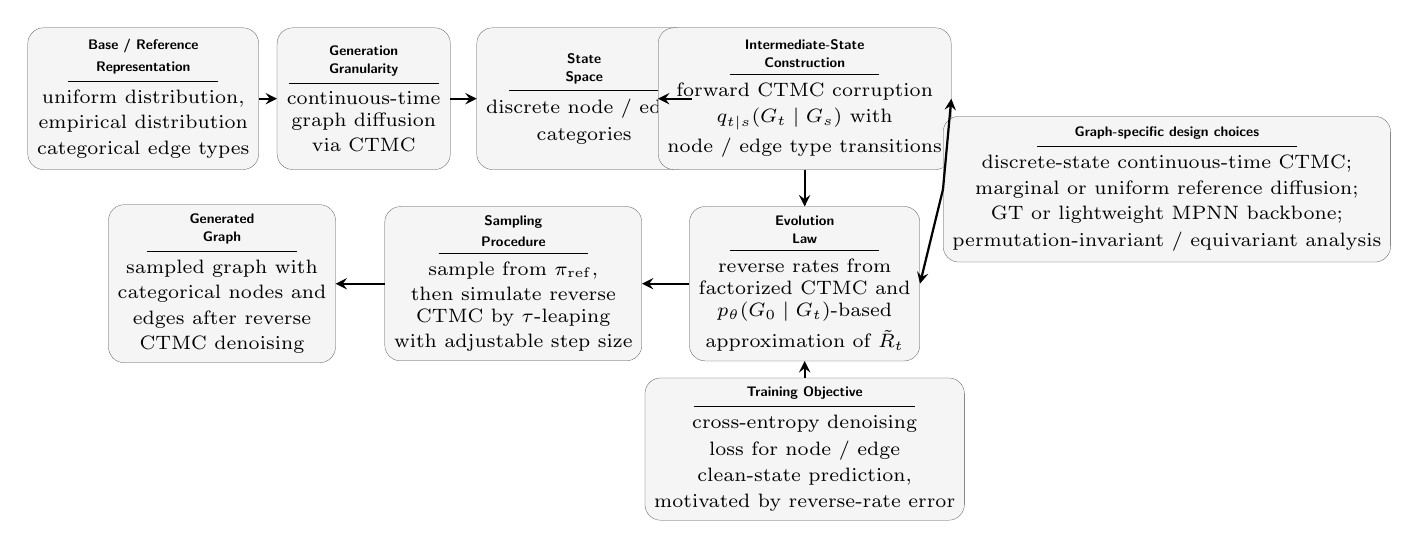
\begin{tikzpicture}[
    >=stealth,
    font=\scriptsize,
    box/.style={
        draw=black!70,
        rounded corners=2mm,
        ultra thin,
        minimum width=2.2cm,
        minimum height=1.8cm,
        align=center,
        fill=gray!8
    },
    side/.style={
        draw=black!70,
        rounded corners=2mm,
        ultra thin,
        minimum width=3.4cm,
        minimum height=1.45cm,
        align=center,
        fill=gray!8
    },
    note/.style={
        draw=black!70,
        rounded corners=2mm,
        ultra thin,
        minimum width=4.1cm,
        minimum height=1.85cm,
        align=center,
        fill=gray!8
    },
    arr/.style={->, thick}
]

% first row
\node[box] (base) at (0,0)
{\shortstack[c]{%
{\sffamily\bfseries\tiny Base / Reference}\\
{\sffamily\bfseries\tiny Representation}\\[-0.2mm]
\rule{1.9cm}{0.2pt}\\[0mm]
uniform distribution, \\
empirical distribution\\
categorical edge types}}; 

\node[box] (time) at (2.8,0)
{\shortstack[c]{%
{\sffamily\bfseries\tiny Generation}\\
{\sffamily\bfseries\tiny Granularity}\\[-0.2mm]
\rule{1.9cm}{0.2pt}\\[0mm]
continuous-time\\
graph diffusion\\
via CTMC}}; 

\node[box] (state) at (5.6,0)
{\shortstack[c]{%
{\sffamily\bfseries\tiny State}\\
{\sffamily\bfseries\tiny Space}\\[-0.2mm]
\rule{1.9cm}{0.2pt}\\[0mm]
discrete node / edge\\
categories}}; 

\node[box] (path) at (8.4,0)
{\shortstack[c]{%
{\sffamily\bfseries\tiny Intermediate-State}\\
{\sffamily\bfseries\tiny Construction}\\[-0.2mm]
\rule{1.9cm}{0.2pt}\\[0mm]
forward CTMC corruption\\
$q_{t|s}(G_t\mid G_s)$ with\\
node / edge type transitions}}; 

% second row
\node[box] (out) at (1.0,-2.35)
{\shortstack[c]{%
{\sffamily\bfseries\tiny Generated}\\
{\sffamily\bfseries\tiny Graph}\\[-0.2mm]
\rule{1.9cm}{0.2pt}\\[0mm]
sampled graph with\\
categorical nodes and\\
edges after reverse\\
CTMC denoising}}; 

\node[box] (sample) at (4.7,-2.35)
{\shortstack[c]{%
{\sffamily\bfseries\tiny Sampling}\\
{\sffamily\bfseries\tiny Procedure}\\[-0.2mm]
\rule{1.9cm}{0.2pt}\\[0mm]
sample from $\pi_{\mathrm{ref}}$,\\
then simulate reverse\\
CTMC by $\tau$-leaping\\
with adjustable step size}}; 

\node[box] (evo) at (8.4,-2.35)
{\shortstack[c]{%
{\sffamily\bfseries\tiny Evolution}\\
{\sffamily\bfseries\tiny Law}\\[-0.2mm]
\rule{1.9cm}{0.2pt}\\[0mm]
reverse rates from\\
factorized CTMC and\\
$p_\theta(G_0\mid G_t)$-based\\
approximation of $\tilde R_t$}}; 

\draw[arr] (base) -- (time);
\draw[arr] (time) -- (state);
\draw[arr] (state) -- (path);
\draw[arr] (path.south) -- ++(0,-0.45) -| (evo.north);
\draw[arr] (evo) -- (sample);
\draw[arr] (sample) -- (out);

% side boxes
\node[side] (train) at (8.4,-4.45)
{\shortstack[c]{%
{\sffamily\bfseries\tiny Training Objective}\\[-0.2mm]
\rule{2.8cm}{0.2pt}\\[0mm]
cross-entropy denoising\\
loss for node / edge\\
clean-state prediction,\\
motivated by reverse-rate error}}; 

\draw[arr] (train.north) -- (evo.south);

\node[note] (graphspec) at (13.0,-1.15)
{\shortstack[c]{%
{\sffamily\bfseries\tiny Graph-specific design choices}\\[-0.2mm]
\rule{3.3cm}{0.2pt}\\[0mm]
discrete-state continuous-time CTMC;\\
marginal or uniform reference diffusion;\\
GT or lightweight MPNN backbone;\\
permutation-invariant / equivariant analysis}}; 

\draw[arr] (graphspec.west) -- (path.east);
\draw[arr] (graphspec.west) -- (evo.east);

\end{tikzpicture}
\caption{DisCo pipeline. DisCo formulates graph generation as a discrete-state continuous-time diffusion process over categorical node and edge types, trained by denoising clean graph prediction and sampled by reverse CTMC simulation with $\tau$-leaping.}
\label{fig:disco_pipeline}
\end{figure*}

\emph{DisCo} \cite{xu2024discrete} is a \emph{discrete-state continuous-time diffusion model} for graph generation that models node and edge types, including non-edges, with a continuous-time Markov chain (CTMC) directly in discrete graph space. It starts from a tractable reference distribution, usually uniform or empirical marginal, and constructs intermediate states through a prescribed continuous-time corruption process defined by shared rate matrices and a time-dependent schedule. To keep inference tractable, the forward and reverse processes are factorized over nodes and edges, with reverse rates estimated by a graph-to-graph neural backbone. The model is trained by cross-entropy denoising of clean node and edge types from noisy graphs at sampled times, and generation proceeds by reverse CTMC simulation with 
$\tau$-leaping, which allows flexible efficiency-quality trade-offs while preserving permutation symmetry under node reordering.


\emph{Evaluation .} DisCo is strong on permutation symmetry, sampling flexibility, and discrete-state faithfulness, making it a principled continuous-time alternative to discrete-time graph diffusion. Its main compromises are the factorized forward process and a continued reliance on standard benchmark metrics for many graph properties, while validity and structural fidelity still depend substantially on the backbone model.

\subsection{Bridge-Based Formulations}
\label{sec:bridge_models}

Bridge-based formulations generate graphs by defining a stochastic interpolation between a reference distribution and the data distribution, typically relative to a chosen diffusion or prior process. Compared with standard denoising or flow-based models, these approaches emphasize the probability path itself and often provide a more global transport perspective on generation. In graph domains, they are particularly relevant when one wants to combine stochasticity, endpoint conditioning, and structured interpolation within a single framework.


\begin{figure*}[htbp]
\centering

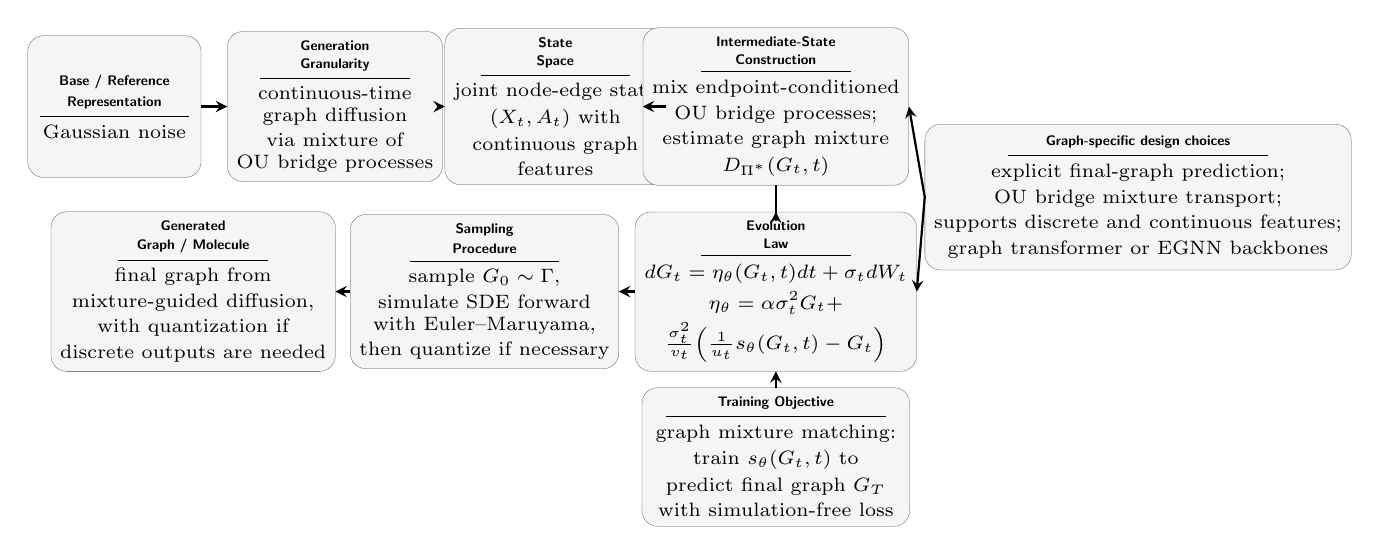
\begin{tikzpicture}[
    >=stealth,
    font=\scriptsize,
    box/.style={
        draw=black!70,
        rounded corners=2mm,
        ultra thin,
        minimum width=2.2cm,
        minimum height=1.8cm,
        align=center,
        fill=gray!8
    },
    side/.style={
        draw=black!70,
        rounded corners=2mm,
        ultra thin,
        minimum width=3.4cm,
        minimum height=1.45cm,
        align=center,
        fill=gray!8
    },
    note/.style={
        draw=black!70,
        rounded corners=2mm,
        ultra thin,
        minimum width=4.1cm,
        minimum height=1.85cm,
        align=center,
        fill=gray!8
    },
    arr/.style={->, thick}
]

% first row
\node[box] (base) at (0,0)
{\shortstack[c]{%
{\sffamily\bfseries\tiny Base / Reference}\\
{\sffamily\bfseries\tiny Representation}\\[-0.2mm]
\rule{1.9cm}{0.2pt}\\[0mm]
Gaussian noise}};

\node[box] (time) at (2.8,0)
{\shortstack[c]{%
{\sffamily\bfseries\tiny Generation}\\
{\sffamily\bfseries\tiny Granularity}\\[-0.2mm]
\rule{1.9cm}{0.2pt}\\[0mm]
continuous-time\\
graph diffusion\\
via mixture of\\
OU bridge processes}};

\node[box] (state) at (5.6,0)
{\shortstack[c]{%
{\sffamily\bfseries\tiny State}\\
{\sffamily\bfseries\tiny Space}\\[-0.2mm]
\rule{1.9cm}{0.2pt}\\[0mm]
joint node-edge state\\
$(X_t,A_t)$ with\\
continuous graph\\ features}}; 

\node[box] (path) at (8.4,0)
{\shortstack[c]{%
{\sffamily\bfseries\tiny Intermediate-State}\\
{\sffamily\bfseries\tiny Construction}\\[-0.2mm]
\rule{1.9cm}{0.2pt}\\[0mm]
mix endpoint-conditioned\\
OU bridge processes;\\
estimate graph mixture\\
$D_{\Pi^\ast}(G_t,t)$}}; 

% second row
\node[box] (out) at (1.0,-2.35)
{\shortstack[c]{%
{\sffamily\bfseries\tiny Generated}\\
{\sffamily\bfseries\tiny Graph / Molecule}\\[-0.2mm]
\rule{1.9cm}{0.2pt}\\[0mm]
final graph from\\
mixture-guided diffusion,\\
with quantization if\\
discrete outputs are needed}}; 

\node[box] (sample) at (4.7,-2.35)
{\shortstack[c]{%
{\sffamily\bfseries\tiny Sampling}\\
{\sffamily\bfseries\tiny Procedure}\\[-0.2mm]
\rule{1.9cm}{0.2pt}\\[0mm]
sample $G_0\sim\Gamma$,\\
simulate SDE forward\\
with Euler--Maruyama,\\
then quantize if necessary}}; 

\node[box] (evo) at (8.4,-2.35)
{\shortstack[c]{%
{\sffamily\bfseries\tiny Evolution}\\
{\sffamily\bfseries\tiny Law}\\[-0.2mm]
\rule{1.9cm}{0.2pt}\\[0mm]
$dG_t=\eta_\theta(G_t,t)dt+\sigma_t dW_t$\\
$\eta_\theta=\alpha\sigma_t^2G_t +$\\
$\frac{\sigma_t^2}{v_t}\!\left(\frac{1}{u_t}s_\theta(G_t,t)-G_t\right)$}}; 

\draw[arr] (base) -- (time);
\draw[arr] (time) -- (state);
\draw[arr] (state) -- (path);
\draw[arr] (path.south) -- ++(0,-0.45) -| (evo.north);
\draw[arr] (evo) -- (sample);
\draw[arr] (sample) -- (out);

% side boxes
\node[side] (train) at (8.4,-4.45)
{\shortstack[c]{%
{\sffamily\bfseries\tiny Training Objective}\\[-0.2mm]
\rule{2.8cm}{0.2pt}\\[0mm]
graph mixture matching:\\
train $s_\theta(G_t,t)$ to\\
predict final graph $G_T$\\
with simulation-free loss}}; 

\draw[arr] (train.north) -- (evo.south);

\node[note] (graphspec) at (13.0,-1.15)
{\shortstack[c]{%
{\sffamily\bfseries\tiny Graph-specific design choices}\\[-0.2mm]
\rule{3.3cm}{0.2pt}\\[0mm]
explicit final-graph prediction;\\
OU bridge mixture transport;\\
supports discrete and continuous features;\\
graph transformer or EGNN backbones}}; 

\draw[arr] (graphspec.west) -- (path.east);
\draw[arr] (graphspec.west) -- (evo.east);

\end{tikzpicture}
\caption{GruM pipeline. GruM models graph generation as a mixture of endpoint-conditioned Ornstein--Uhlenbeck bridge processes and learns a graph mixture that predicts the final graph structure, guiding the diffusion trajectory toward valid topology.}
\label{fig:grum_pipeline}
\end{figure*}

\emph{GruM} \cite{jo2023graph} is a \emph{bridge-based} graph generator that models generation as a \emph{mixture of endpoint-conditioned diffusion processes}, specifically an Ornstein--Uhlenbeck bridge mixture transporting samples from a prior to the data distribution. It operates in a \emph{relaxed continuous graph space}, where node features and adjacency matrices evolve continuously and are quantized only at the end if needed, starting from an arbitrary prior that is instantiated in practice as Gaussian noise. Intermediate states follow a \emph{bridge path} guided by a predicted graph mixture, and the evolution is governed by an SDE whose drift depends on this predicted terminal graph. Training uses a \emph{likelihood-based bridge objective} that reduces to matching the predicted graph mixture to the terminal graph, while sampling simulates the learned SDE with Euler--Maruyama integration from the prior toward the data distribution. Its main graph-specific strengths are the explicit modeling of terminal graph topology, support for both discrete structure and continuous features, and graph neural parameterization that avoids reliance on a fixed node ordering.

\emph{Evaluation .} GruM is especially strong on complex dependencies, topology-aware generation, and validity-sensitive graph synthesis, because it explicitly learns a prediction of the final graph rather than only denoising intermediate noise. Its main limitation is that permutation symmetry is handled more practically than theoretically, and the method remains a deep generative model whose control and interpretability, while improved, are still not complete.

\label{sec:ct_summary}



% =========================
\section{Comparative Taxonomy of Time-Dependent Graph Generation}
\label{sec:comparative_taxonomy}

The preceding sections show that discrete-time and continuous-time graph generators are best viewed as two complementary ways of specifying a temporal transformation from a simple reference distribution to a target graph distribution. Across both perspectives, the main modeling question is the same: how to define a trajectory over intermediate states, how to learn the local rule governing that trajectory, and how to recover valid graph samples efficiently at the end. What differs is the parameterization of time, the form of the local dynamics, the state space in which the process evolves, and the degree to which graph structure is preserved explicitly during generation.



\subsection{Comparison by Time Domain}
\label{sec:compare_time_domain}

The most immediate distinction concerns the representation of time. Discrete-time methods define generation through a finite sequence of transitions, so the number of denoising, editing, or refinement steps is part of the model design itself. This gives them a direct and often interpretable control over generation budgets and intermediate states. In graph settings, this is especially attractive when intermediate objects are intended to remain meaningful graphs, as in edge-editing, categorical denoising, masking, or constrained reverse refinement. Representative examples include GraphGUIDE, DiGress, ConStruct, EDGE, GraphARM, and LayerDAG.

Continuous-time methods instead define a process over a continuous interval, typically through an ODE, an SDE, or a continuous-time jump process. Here the learned model is conceptually separated from the numerical procedure used to simulate it. This gives greater flexibility in solver design, stochasticity control, and the choice of simulation budget, but also introduces sensitivity to discretization error and computational overhead. In practice, continuous-time formulations are especially appealing when one wants to connect graph generation to transport, diffusion, or stochastic-process viewpoints, as seen in CGF, ModFlow, CatFlow, BWFlow, GGBall, GraphBSI, DisCo, and GruM.

A useful way to interpret this contrast is that discrete-time models usually make temporal resolution an explicit modeling choice, whereas continuous-time models treat temporal resolution primarily as an inference-time approximation choice. This difference influences not only efficiency, but also how tightly training and sampling are coupled.

\subsection{Comparison by evolution law}

A second key axis is the form of the evolution law. In discrete-time models, the local dynamics are typically implemented as finite-step transition kernels, denoising updates, autoregressive expansions, or editing rules. These are naturally aligned with graph manipulations such as edge flipping, node masking, edge absorption, or layerwise construction. As a result, discrete-time generators often offer transparent step-by-step semantics and are comparatively easy to adapt when one needs explicit graph edits or constrained reverse moves.

In continuous-time models, the evolution law can take several forms. ODE-based methods describe deterministic transport through a velocity field, as in continuous normalizing flows and flow matching. SDE-based models describe stochastic continuous dynamics through drift and diffusion terms, typically learned through score or denoising objectives. CTMC-based methods define the evolution directly on discrete states through time-dependent jump rates. Bridge-based models emphasize endpoint-conditioned stochastic transport, often making the probability path itself a central modeling object. This diversity makes the continuous-time literature more heterogeneous, but also more expressive from a modeling perspective.

At a high level, ODE-based methods emphasize smooth transport and flexible path design, SDE-based methods emphasize stochastic refinement and generative robustness, CTMC-based methods preserve discrete graph semantics throughout generation, and bridge-based methods provide a global transport perspective between source and target distributions.


\begin{table*}[!t]
\centering
\caption{Representative continuous-time graph generative models organized by the main taxonomy axes.}
\label{tab:taxonomy_models_continuous}
\small
\renewcommand{\arraystretch}{1.15}
\setlength{\tabcolsep}{4pt}
\begin{tabularx}{\textwidth}{|
    >{\raggedright\arraybackslash}p{2.8cm}|
    >{\raggedright\arraybackslash}p{2.9cm}|
    >{\raggedright\arraybackslash}p{2.5cm}|
    >{\raggedright\arraybackslash}X|}
\hline
\textbf{Method} & \textbf{Evolution Law} & \textbf{State Space} & \textbf{Intermediate-State Construction} \\
\hline
CGF~\cite{deng2019continuous} & ODE-based continuous normalizing flow & Relaxed graph space & Continuous transport path induced by neural ODE dynamics \\
\hline
ModFlow~\cite{verma2022modular} & ODE-based continuous normalizing flow & Relaxed graph space & Continuous transport path over coupled node trajectories \\
\hline
CatFlow / VFM~\cite{eijkelboom2024vfm} & ODE-based flow matching / variational velocity model & Relaxed categorical graph space & Coupling- or interpolant-based construction \\
\hline
GGFlow~\cite{hou2024ggflow} & Discrete-state flow matching / conditional probability velocity & Discrete graph space & Coupling-based categorical interpolation with OT-informed endpoint pairing \\
\hline
DeFoG~\cite{qin2025defog} & CTMC / discrete flow matching & Discrete graph space & Prescribed linear interpolation path with jump-process reverse denoising \\
\hline
BWFlow~\cite{bwflow} & ODE-based flow matching & Relaxed or mixed graph space & Bures--Wasserstein interpolant-based construction \\
\hline
GGBall~\cite{ggball} & Riemannian ODE-based flow matching & Hyperbolic latent space & Geometry-aware geodesic interpolant \\
\hline
EDP-GNN~\cite{niu2020permutation} & Score-based stochastic refinement / annealed Langevin dynamics & Continuous relaxed adjacency space & Prescribed Gaussian noising path \\
\hline
PRODIGY~\cite{sharma2024plug} & Reverse-time SDE with projection-guided correction & Relaxed graph space & Prescribed forward noising path with projection-corrected reverse updates \\
\hline
GraphBSI~\cite{song2025smooth} & Drift--diffusion process in belief space & Relaxed categorical belief space & Smooth belief-space interpolation induced by Bayesian updates \\
\hline
DisCo~\cite{xu2024discrete} & Factorized CTMC with learned reverse rates & Discrete categorical graph space & Jump-process path \\
\hline
GruM~\cite{jo2023graph} & Bridge SDE / OU-bridge mixture dynamics & Relaxed graph space & Bridge-based construction relative to prior and endpoint mixture \\
\hline
\end{tabularx}
\end{table*}

\subsection{Comparison by State Space}
\label{sec:compare_state_space}



\begin{table*}[!t]
\centering
\caption{Representative discrete-time graph generative models organized by the main taxonomy axes.}
\label{tab:taxonomy_models_discrete}
\small
\renewcommand{\arraystretch}{1.15}
\setlength{\tabcolsep}{4pt}
\begin{tabularx}{\textwidth}{|
    >{\raggedright\arraybackslash}p{2.8cm}|
    >{\raggedright\arraybackslash}p{2.9cm}|
    >{\raggedright\arraybackslash}p{2.5cm}|
    >{\raggedright\arraybackslash}X|}
\hline
\textbf{Method} & \textbf{Evolution Law} & \textbf{State Space} & \textbf{Intermediate-State Construction} \\
\hline
GraphGUIDE~\cite{tseng2023graphguide} & Bernoulli transition kernels / reverse denoising & Discrete graph space & Prescribed Bernoulli noising path \\
\hline
ConStruct~\cite{madeira2024generative} & Transition kernels / reverse denoising with projector & Discrete graph space & Edge-absorbing noising path with constrained reverse refinement \\
\hline
EDP~\cite{haefeli2022diffusion} & Transition kernels / reverse denoising & Discrete graph space & Prescribed discrete noising path to Erd\H{o}s--R\'enyi prior \\
\hline
DiGress~\cite{vignac2022digress} & Transition kernels / reverse denoising & Discrete attributed graph space & Prescribed discrete noising path with marginal-preserving transitions \\
\hline
EDGE~\cite{chen2023efficient} & Transition kernels / reverse denoising with active-node factorization & Discrete graph space & Edge-removal path to empty-graph prior with degree-guided reverse refinement \\
\hline
GBD~\cite{liu2024advancing} & Reverse beta denoising transitions & Continuous bounded graph space & Prescribed multiplicative beta noising path with concentration modulation \\
\hline
GGSD~\cite{minello2024generating} & Spectral reverse denoising transitions & Relaxed spectral graph space & Prescribed Gaussian noising path in Laplacian spectral space \\
\hline
GraphARM~\cite{kongautoregressive} & Absorbing diffusion / autoregressive reverse kernel & Discrete graph space & Node-absorbing path with reverse node-wise reconstruction \\
\hline
LayerDAG~\cite{li2024layerdag} & Autoregressive layer transitions + denoising kernels & Discrete DAG space & Layerwise transition path with inner discrete noising \\
\hline
MAGNet~\cite{hetzel2025magnet} & Latent-conditioned hierarchical update rules & Latent space & Learned hierarchical transition path over scaffold and motif structure \\
\hline
\end{tabularx}
\end{table*}

State space remains one of the most consequential design choices in time-dependent graph generation. Some methods evolve directly in discrete graph space, where each intermediate state is itself a graph or attributed graph. This is the clearest setting for GraphGUIDE, DiGress, ConStruct, EDGE, GGFlow, DeFoG, and DisCo. The main advantage is faithfulness to the graph domain: intermediate states are combinatorial objects, structural constraints can often be expressed directly, and reverse updates can be interpreted in graph-theoretic terms. The main disadvantage is that optimization and parameterization become more difficult as graph size and attribute complexity grow.

Other methods evolve in continuous relaxations of graph variables, such as softened adjacency matrices, node-score vectors, bounded continuous graph variables, spectral representations, or belief logits. This is common in EDP-GNN, GBD, GGSD, CGF, ModFlow, CatFlow, GraphBSI, PRODIGY, and GruM. These formulations are more compatible with ODEs, SDEs, and gradient-based learning, but they create a gap between the evolving state and the final discrete graph, which must later be closed through thresholding, quantization, decoding, or projection.

A third option is latent-space evolution, where transport is performed over learned graph embeddings rather than graph variables themselves. GGBall is the clearest example in the current survey. Latent evolution may improve scalability and representation power, especially when geometry-aware interpolation is helpful, but it shifts the burden to the encoder--decoder pipeline and makes structural guarantees less direct.

Overall, discrete graph space usually offers stronger interpretability and more direct validity control, while relaxed or latent spaces offer greater compatibility with continuous dynamics and richer geometric modeling.


\subsection{Comparison by intermediate-state construction}

The reviewed literature also differs substantially in how intermediate states are constructed. In many discrete-time diffusion models, the path is prescribed in advance through a corruption process, such as Bernoulli edge perturbation, categorical noising, edge absorption, Gaussian perturbation, or beta diffusion. The learning problem is then mainly to approximate the reverse process. This makes supervision simple and stable, but it also ties the model to the chosen forward path.

Flow-matching and transport-based methods instead place more weight on the design of the probability path itself. Their intermediate states are induced by an interpolant, a coupling, or a geometry-aware displacement between source and target samples. CatFlow uses a simple interpolation in relaxed categorical space, GGFlow uses OT-informed conditional interpolation in discrete graph space, BWFlow uses a Bures--Wasserstein interpolant in a graph-aware relaxed space, and GGBall uses geodesic interpolation in hyperbolic latent space. In these models, path quality is often as important as network architecture.

Bridge-based methods add a different perspective: instead of prescribing a simple corruption path or a deterministic interpolant, they define intermediate distributions through a stochastic process conditioned on endpoints or endpoint mixtures. GruM illustrates this viewpoint in graph generation by using an OU-bridge mixture guided by terminal-graph prediction.

Finally, CTMC and other jump-based models construct intermediate states through discrete events rather than smooth interpolation. This makes them especially natural for categorical graph generation, where the core state variables are already discrete.


\subsection{Comparison by Training Objective}
\label{sec:compare_training}


Different temporal formulations induce different learning objectives. Discrete-time denoising methods are commonly trained by reconstruction or cross-entropy objectives that predict the clean graph, the clean node/edge labels, or the next reverse update from a corrupted intermediate state. This is the dominant pattern in GraphGUIDE, DiGress, ConStruct, EDGE, and related models.

Continuous-time score-based methods typically learn local information about the evolving density, either through denoising score matching or equivalent denoising objectives. ODE-based likelihood models instead optimize exact or approximate log-likelihoods via change-of-variables arguments, as in CGF and ModFlow. Flow-matching methods learn the local generator of a prescribed path, often through velocity regression or, in categorical settings, through endpoint-prediction objectives that induce the local flow. CTMC-based methods generally rely on denoising or marginal-prediction losses that support tractable reverse-rate approximation. Bridge-based methods tend to optimize likelihood- or KL-related objectives defined relative to an endpoint-conditioned stochastic process.

Thus, the training objective is not merely an implementation detail: it determines whether the model learns a reverse kernel, a score, a velocity field, a rate operator, or a terminal-state predictor, and this in turn shapes the interpretability, flexibility, and computational profile of the method.


\subsection{Comparison by Sampling Behavior}
\label{sec:compare_sampling}

The practical behavior of these models is often most visible at sampling time. Discrete-time generators usually perform a finite sequence of reverse transitions, edits, or refinements. This often makes the trade-off between speed and quality easy to interpret, and it supports meaningful inspection of intermediate states. However, long reverse chains can still be expensive, especially for dense attributed graphs.

Continuous-time models are typically sampled through numerical simulation. ODE-based methods require integration, SDE-based methods require reverse-time stochastic simulation or associated probability-flow ODE solvers, and CTMC-based methods require jump simulation, Euler stepping, or $\tau$-leaping. This makes continuous-time methods more flexible in principle, because solver choice, step size, and stochasticity can often be changed without retraining, but also more sensitive to inference-time design.

A particularly important distinction is whether training and sampling are tightly coupled. In many discrete-time denoising models, the forward process, training objective, and reverse sampler are tightly linked. By contrast, several continuous-time methods partly decouple these choices. Flow matching avoids full trajectory simulation during training, and methods such as DeFoG and DisCo explicitly allow post-training changes in simulation behavior. This decoupling is one of the practical strengths of continuous-time formulations.

\subsection{Comparison by Graph Constraints}
\label{sec:compare_constraints}

Across both time regimes, graph-specific design choices remain central. The first is symmetry handling. Since graphs admit many equivalent representations under node permutation, models must either be permutation equivariant, rely on invariant representations, impose canonicalization, or otherwise reduce ordering sensitivity. Many modern methods rely on graph neural or transformer backbones to mitigate this issue, but few eliminate it entirely.

The second is dependency modeling. Graph generation requires capturing dependencies among nodes, edges, attributes, and often higher-order structural motifs. Methods such as BWFlow, GGBall, GGFlow, ModFlow, and GruM illustrate different ways of strengthening dependency modeling, whether through geometry-aware transport, discrete conditional paths, coupled node dynamics, or endpoint-aware stochastic transport.

The third is structural validity and controllability. Some methods directly preserve or project onto constraint sets, as in ConStruct and PRODIGY; others encourage validity indirectly through representation choice, priors, or decoder design. In general, hard validity guarantees remain the exception rather than the rule, especially outside specialized domains such as DAG generation.

The fourth is scalability and sampling efficiency. Sparse priors, factorized reverse updates, active-node strategies, spectral representations, latent transport, and solver flexibility all serve as mechanisms for coping with large graph spaces. Yet no single strategy resolves the tension between expressiveness, exact structural control, and computational efficiency.

\subsection{Synthesis}

Taken together, the survey suggests that discrete-time methods currently offer the clearest path when interpretability, direct graph manipulation, and explicit constraint handling are primary goals, whereas continuous-time methods offer a broader and often more principled modeling toolkit for transport design, stochastic refinement, solver flexibility, and geometry-aware generation. Neither perspective dominates universally. Instead, the most suitable choice depends on which aspect of graph generation is prioritized: exact graph-space faithfulness, transport smoothness, controllability, efficiency, or structural inductive bias.

% =========================
\section{Evaluation Protocols and Experimental Practice}
\label{sec:evaluation_protocols}

Evaluating graph generative models remains challenging because generation quality is multi-faceted and often depends on the graph domain, the representation, and the intended downstream task. In practice, evaluation is rarely captured by a single number: a model may match global graph statistics while still producing low-quality, repetitive, or structurally invalid samples. For this reason, we organize this section around evaluation metrics, benchmark design, illustrative empirical comparison, and practical issues of efficiency and reproducibility.

\subsection{Evaluation metrics}
\label{subsec:evaluation_metrics}

A strong evaluation metric for graph generative models should reflect how well generated graphs match the reference distribution in terms of \emph{fidelity} and \emph{diversity}, while also being \emph{sample efficient} and \emph{computationally efficient} \cite{thompson2022evaluation}. These criteria are broadly aligned with the desiderata discussed in \cite{obray2022evaluation}, which summarize a good graph-generation evaluation metric in terms of \emph{expressivity}, \emph{robustness}, and \emph{efficiency}. In this view, fidelity and diversity can be understood as aspects of expressivity, while sample and computational efficiency refine the broader notion of efficiency, so the two perspectives are complementary rather than conflicting.

Broadly, evaluation metrics for graph generation can be grouped into four families: \emph{descriptor-based distributional metrics}, \emph{learned-feature metrics}, \emph{classifier-based metrics}, and \emph{intrinsic-quality-based metrics}.

\paragraph{Descriptor-based distributional metrics.}
These methods compute hand-crafted graph statistics for each graph and then compare the empirical distributions of those statistics between generated and reference sets. Their main advantage is interpretability, since each metric can often be traced back to a recognizable graph property. However, they also suffer from well-known limitations: performance depends strongly on the selected descriptors, multiple descriptor-specific scores are often needed, and kernel-based distances such as Maximum Mean Discrepancy (MMD) or Wasserstein distance can be sensitive to kernel choice and bandwidth selection \cite{krimmel2025polygraph}. Common graph descriptors include degree distributions, clustering coefficients, orbit counts, and Laplacian spectra.

\paragraph{Learned-feature metrics.}
Here graphs are first embedded into a learned representation space, often using graph neural networks, and then compared in that feature space. These metrics aim to capture richer dependencies than hand-crafted statistics alone, potentially incorporating node and edge attributes more naturally. Depending on the setup, the encoder may be randomly initialized, self-supervised, or pretrained. Learned-feature metrics can therefore offer a more expressive view of graph similarity, although they may be less interpretable and can inherit biases from the chosen encoder architecture or training procedure. The comparison can again use MMD or Fr\'echet-style distances. Representative feature extractors include random GNNs \cite{thompson2022evaluation}, contrastively trained GNNs \cite{shirzad2022evaluating}, and other pretrained or self-supervised graph encoders \cite{krimmel2025polygraph}.

\paragraph{Classifier-based metrics.}
These methods recast evaluation as a discrimination problem between generated and reference samples. Instead of directly computing a kernel distance between two empirical distributions, they train a classifier to separate real from generated graphs and use the classifier's performance or likelihood-based objective as an estimate of distributional discrepancy \cite{krimmel2025polygraph}. This perspective can provide bounded and more easily interpretable scalar scores, and it is especially appealing when multiple descriptors or representations must be combined. At the same time, classifier-based evaluation depends on the capacity of the discriminator, sample size, and train--test protocol, and therefore requires careful reporting.

\paragraph{Intrinsic-quality-based metrics.}
In addition to comparing generated and reference distributions, many graph generation papers report intrinsic quality indicators that assess the generated set itself. Common examples include \emph{validity}, \emph{uniqueness}, and \emph{novelty} \cite{guo2022systematic}. Validity measures whether generated samples satisfy structural or domain-specific rules; uniqueness measures the proportion of non-duplicate generated samples; and novelty measures the proportion of generated samples that do not simply reproduce training examples. These metrics are especially common in molecular generation, but they also appear in general graph generation when validity can be defined through benchmark-specific graph properties such as planarity, connectivity, or community structure. For example, GruM evaluates general graph generation using both MMD-based structural statistics and a combined V.U.N.\ criterion, and reports validity, uniqueness, and novelty for molecular benchmarks \cite{jo2024grum}.

In practice, these metric families capture different aspects of generation quality. Descriptor-based, learned-feature, and classifier-based metrics primarily assess how closely the generated distribution matches the reference distribution, whereas intrinsic-quality-based metrics assess whether the generated samples themselves are structurally meaningful, non-trivial, and diverse. A sound evaluation protocol should therefore avoid relying on only one type of metric.

Representative benchmarks in graph generation include synthetic datasets such as planar graphs, stochastic block models, and tree-like families, as well as citation, protein-contact, or ego-network collections used as generic graph benchmarks. These benchmarks are useful because they make it possible to study how metrics respond to controlled perturbations, but they also expose a recurring issue in the literature: benchmark sizes are often small, making metric variance and ranking instability an important concern.

\subsection{Benchmark design and reporting practice}
\label{subsec:benchmark_reporting}

Beyond the choice of metric, evaluation quality depends critically on how experiments are designed and reported. Two papers using the same model family may reach different conclusions simply because they use different dataset splits, sample sizes, kernel settings, or variance estimation procedures. Consequently, benchmark design and reporting practice are not secondary details, but central components of credible graph generation evaluation.

A first issue is the choice of dataset and split protocol. Synthetic benchmarks are useful because they provide controllable distributions and allow large-scale sampling, but they may fail to reflect the structural richness of real-world applications. Real-world benchmarks offer more realistic distributions, yet they are often smaller and less standardized. In task-specific settings, split choice can be especially important: random splits may overestimate generalization, while scaffold, temporal, or structure-aware splits may provide a more realistic picture of model performance.

A second issue is the number of generated and reference samples used for evaluation. Many graph generation papers evaluate on relatively small sample sets, which can introduce high variance into descriptor distributions and instability into kernel-based distances such as MMD. This makes it essential to report not only mean scores but also uncertainty estimates, subsampling variance, confidence intervals, or repeated-trial statistics whenever possible. Without such information, apparent model improvements may simply reflect estimator noise.

A third issue concerns hyperparameter disclosure and reproducibility. When evaluation relies on kernel methods, authors should specify the chosen descriptors, kernels, bandwidths, and any tuning strategy. When learned-feature or classifier-based metrics are used, the feature extractor, discriminator, training protocol, and test procedure should be described clearly enough to enable replication. Likewise, post-processing steps, invalid-sample filtering, rejection procedures, and decoding heuristics should be explicitly reported because they can materially change the final evaluation.

A fourth issue is fair comparison across model classes. Different generative families---such as autoregressive, diffusion, latent-variable, flow-based, or discrete editing models---may differ not only in sample quality but also in generation budget, post-processing requirements, and the extent to which validity is enforced by construction. Benchmark protocols should therefore avoid comparing methods under mismatched computational budgets or incompatible reporting conventions.

Overall, good experimental practice requires that evaluation protocols be documented with the same rigor as model architectures. In graph generation, where metrics are numerous and often imperfect, careful reporting is essential for making results interpretable and comparable across papers.

\subsection{Illustrative empirical comparison on synthetic benchmarks}
\label{subsec:illustrative_benchmark}

To complement the methodological discussion above, we include a small-scale empirical comparison under a unified protocol on two synthetic graph benchmarks. The goal of this experiment is not to provide a definitive ranking of all graph generative models, but to illustrate how conclusions may change across metric families even when models are evaluated on the same datasets with the same sample budget.

We recommend selecting a representative subset of time-dependent graph generators spanning the main families discussed in this survey. A practical benchmark set may include three discrete-time models (e.g., GraphGUIDE, DiGress, and ConStruct) and three continuous-time models (e.g., EDP-GNN, DisCo, and GruM). This yields a manageable yet diverse comparison across discrete denoising, score-based continuous-time diffusion, discrete-state CTMC generation, and bridge-based stochastic generation.

For the synthetic datasets, we recommend two widely used graph benchmarks with complementary structural biases, such as stochastic block models (SBM) and planar graphs. These datasets provide controlled target distributions and make it easier to assess metric sensitivity, ranking stability, and the interaction between structure preservation and model inductive bias.

The empirical comparison should evaluate at least four metric families:
(i) descriptor-based distributional metrics, such as MMD on degree distributions, clustering coefficients, orbit counts, and spectral statistics;
(ii) learned-feature metrics, computed in a graph-neural embedding space;
(iii) classifier-based metrics, which estimate how easily generated and reference graphs can be distinguished; and
(iv) intrinsic-quality-based metrics, such as validity or benchmark-specific feasibility rates.

Table~\ref{tab:synthetic_benchmark_setup} summarizes the proposed model and dataset setup, while Table~\ref{tab:synthetic_benchmark_results} reports the main quantitative results.

\begin{table}[http]
\centering
\caption{Illustrative synthetic benchmark setup.}
\label{tab:synthetic_benchmark_setup}
\small
\begin{tabular}{l l l}
\toprule
Category & Representative models & Notes \\
\midrule
Discrete-time & GraphGUIDE, DiGress, ConStruct & denoising / constrained diffusion \\
Continuous-time & EDP-GNN, DisCo, GruM & score-based / CTMC / bridge-based \\
Datasets & SBM, Planar & synthetic graph benchmarks \\
\bottomrule
\end{tabular}
\end{table}


\begin{table*}[t]
\centering
\caption{Aggregated empirical comparison results.}
\label{tab:synthetic_benchmark_results}
\small
\begin{tabular}{l l r r r r r r}
\toprule
Dataset & Model & Classifier separation & Degree MMD & Clustering MMD & Orbit MMD & Spectral MMD & Learned-feature MMD \\
\midrule
Planar & ConStruct & 0.000000 & 0.000627 & 0.001017 & 0.221169 & 0.014274 & 1.400688 \\
Planar & DiGress & 0.318966 & 0.000534 & 0.001015 & 0.178744 & 0.014051 & 0.475956 \\
Planar & DisCo & 0.224138 & 0.000602 & 0.001008 & 0.180737 & 0.013334 & 0.656563 \\
Planar & EDP-GNN & 0.000000 & 0.001006 & 0.017639 & 0.218053 & 0.014307 & 1.517441 \\
Planar & GraphGUIDE & 0.232759 & 0.000599 & 0.001010 & 0.180585 & 0.013956 & 0.478038 \\
Planar & GruM & 0.129310 & 0.000416 & 0.000790 & 0.152959 & 0.007125 & 0.431248 \\
\midrule
SBM & ConStruct & 0.000000 & 0.000030 & 0.000026 & 0.038882 & 0.002031 & 1.115000 \\
SBM & DiGress & 0.517241 & -0.000003 & 0.000022 & 0.002495 & 0.000270 & 0.024221 \\
SBM & DisCo & 0.362069 & 0.000006 & 0.000035 & 0.006252 & 0.001028 & 0.373067 \\
SBM & EDP-GNN & 0.000000 & 0.810661 & 0.810671 & 0.602778 & 0.730083 & 0.807446 \\
SBM & GraphGUIDE & 0.387931 & 0.000040 & 0.178352 & 0.010386 & 0.001606 & 0.457012 \\
SBM & GruM & 0.068966 & -0.000005 & 0.000151 & 0.015455 & 0.001932 & 0.617231 \\
\bottomrule
\end{tabular}
\end{table*}

\subsection{Efficiency and scalability}
\label{subsec:efficiency_scalability}

Evaluation should also account for the practical cost of training and using graph generative models. A model that achieves strong fidelity on small graphs but becomes prohibitively slow or memory-intensive on larger ones may be of limited practical value. For this reason, efficiency and scalability deserve explicit discussion alongside sample-quality metrics.

Training efficiency concerns the computational resources required to fit the model, including optimization time, hardware demand, and memory consumption. These costs can vary widely across generative paradigms: autoregressive methods may incur sequential training or decoding overhead, diffusion models often require many denoising steps, and flow-based or continuous-time approaches may trade off stronger likelihood structure against integration cost. Reporting training efficiency helps contextualize whether improvements in generation quality come at acceptable computational expense.

Sampling efficiency is equally important. Some methods can produce samples in a single pass, while others require iterative refinement, long Markov chains, or repeated validity correction. In practice, sampling cost may determine whether a model can be used for large-scale candidate generation or interactive design workflows. Therefore, evaluation should ideally report generation throughput, wall-clock sampling time, and the dependence of sampling cost on graph size.

Scalability with respect to graph size and attribute richness is another major concern. Many models perform well on small benchmark graphs but struggle when the number of nodes, edges, or labels increases. Memory requirements, batching limitations, and quadratic or worse computational growth can all become bottlenecks. Accordingly, a convincing evaluation should indicate how performance and cost change as graphs become larger or more complex.

Finally, evaluation itself can be expensive. Descriptor computation, orbit counting, learned embedding extraction, and repeated kernel or classifier-based comparisons may incur substantial runtime, especially when uncertainty estimates are reported. Thus, efficiency should be considered not only for the generator but also for the overall evaluation pipeline. This is particularly important when models are tuned through repeated evaluation during development.

In summary, efficiency and scalability are not merely engineering considerations. They shape which graph generative models are viable in practice and should therefore be reported as first-class evaluation dimensions.

\subsection{Summary of recommendations}
\label{subsec:evaluation_recommendations}

Based on the discussion above, a sound evaluation protocol for graph generative models should report more than a single distribution-matching score. At minimum, authors should clarify the evaluation objective and report metrics that reflect both distributional similarity and intrinsic sample quality.

In particular, it is advisable to combine interpretable descriptor-based statistics with more expressive learned-feature or classifier-based metrics when possible, and to complement them with intrinsic-quality-based measures such as validity, uniqueness, and novelty whenever these are meaningful for the task. Evaluation should also be tied to clear benchmark protocols, including dataset choice, split strategy, sample budget, and uncertainty estimation.

Authors should disclose all metric-specific design choices, including descriptors, kernels, hyperparameters, feature extractors, classifiers, filtering rules, and post-processing steps. Repeated trials or subsampling-based uncertainty estimates should be included whenever metric variance may affect model ranking. Finally, efficiency should be reported alongside sample quality, including training cost, sampling cost, graph-size scaling, and the computational overhead of the evaluation pipeline itself.

Taken together, these practices can make graph generation results more interpretable, reproducible, and comparable across model families and application domains.


\section{Applications of Time-Dependent Graph Generation}
\label{sec:applications}

Time-dependent graph generation has found particularly strong applications in scientific domains where the target object is relational, high-dimensional, and subject to nontrivial structural constraints. In these settings, generative models are useful not only for unconditional sampling, but also for conditional design, optimization, completion, and simulation of structured objects. Although the application landscape is still expanding, current work is especially concentrated in molecular design, protein design and structural biology, and materials generation.

\subsection{Molecular Design and Structure-Based Drug Design}
\label{sec:app_molecular}

Molecular design is the most established application area for time-dependent graph generation, especially in de novo drug design and structure-based drug design. In this setting, atoms are represented as nodes and bonds as edges, while generation aims to produce chemically valid molecules that satisfy desired constraints such as novelty, synthesizability, drug-likeness, or target-specific binding affinity \cite{alakhdar2024diffusion}. Time-dependent generative models are particularly attractive in this setting because they support iterative refinement of molecular structure and can naturally accommodate conditional information, including physicochemical properties, molecular scaffolds, and protein binding pockets.

A major branch of this literature focuses on \emph{structure-based drug design} (SBDD), where the model generates ligands conditioned on a target protein pocket. In this setting, time-dependent generation is used not merely to sample plausible molecules, but to guide the search toward compounds that fit the local geometry and interaction landscape of the binding site. For example, FLAG generates ligands fragment-by-fragment using a motif vocabulary and explicit 3D pocket context, improving the realism of generated substructures while retaining competitive binding-related performance \cite{zhang2023flag}. IRDIFF extends this target-aware setting by incorporating retrieval augmentation, using reference ligands with favorable binding affinities to steer diffusion-based generation toward better protein-specific candidates \cite{huang2024irdiff}. VoxBind shows that this application can also be approached through voxelized molecular representations rather than point clouds, and reports improved diversity, fewer steric clashes, and stronger binding affinity on SBDD benchmarks \cite{pinheiro2024voxbind}.

Recent work also shows that this application area is broader than target-aware ligand generation alone. DECOMPOPT formulates structure-based molecular optimization with a controllable and decomposed diffusion model, explicitly covering both de novo design and controllable tasks such as R-group optimization and scaffold hopping \cite{zhou2024decompopt}. More generally, molecular applications increasingly blur the boundary between generation and downstream molecular assessment. UniGEM argues that molecular generation and molecular property prediction should be treated jointly rather than as isolated tasks, and proposes a unified diffusion-based framework that improves both generative and predictive performance \cite{feng2025unigem}. This reflects a broader shift in molecular applications: graph generation is no longer viewed only as distribution learning over molecules, but as part of a larger design pipeline involving controllable generation, screening, optimization, and property-aware refinement.

Overall, molecular design remains the clearest demonstration of the practical value of time-dependent graph generation. At the same time, it also exposes its main limitations: validity constraints are often only partially enforced, target-specific utility can diverge from generic distributional fidelity, and evaluation must often combine intrinsic graph quality with chemically meaningful and task-specific criteria.

\subsection{Protein Design and Structural Biology}
\label{sec:app_protein}

A second major application area is protein design and structural biology. In contrast to small-molecule generation, these tasks place greater emphasis on large-scale 3D geometry, structural diversity, conformational flexibility, and downstream designability. Time-dependent generative models have become increasingly important here because they provide a principled way to sample complex distributions over protein structures rather than predicting only a single deterministic state.

One prominent use case is \emph{de novo protein backbone generation}. In this setting, the goal is to generate novel backbone structures that are designable, diverse, and sufficiently realistic to support subsequent sequence design or experimental validation. Genie showed early evidence that equivariant diffusion over residue-centered geometric representations can produce protein backbones with improved designability, novelty, and diversity relative to earlier baselines \cite{lin2023genie}. More recent works extend this line in different directions. FoldFlow formulates protein backbone generation through flow matching on $SE(3)$ and demonstrates that transport-based continuous-time modeling can generate high-quality, designable, and novel proteins \cite{bose2024foldflow}. Proteus improves practical performance by combining diffusion with stronger architectural inductive biases, emphasizing both designability and efficiency in de novo protein backbone generation \cite{wang2024proteus}. Prote\'ina pushes further toward scale and controllability by developing a large-scale flow-based protein backbone generator with hierarchical fold conditioning, enabling both unconditional and controlled protein structure synthesis at much larger scale \cite{geffner2025proteina}.

A second line of work focuses less on static backbone design and more on \emph{protein conformational landscapes}. In many biological settings, function depends not on a single folded state but on an ensemble of accessible conformations or on transitions between metastable states. Time-dependent generative models are especially well suited to this regime because they can model distributions over structures and trajectories rather than single outputs. AlphaFLOW adapts flow matching to protein structure prediction models in order to generate conformational ensembles, showing that time-dependent generative modeling can capture protein flexibility and serve as a proxy for some expensive simulation workloads \cite{jing2024alphaflow}. CONFDIFF likewise incorporates force guidance into an $SE(3)$ diffusion model to generate protein conformations that are both diverse and better aligned with low-energy regions of the landscape \cite{wang2024confdiff}. MDGEN broadens this perspective further by formulating direct generative modeling of molecular dynamics trajectories, enabling applications such as forward simulation, interpolation, upsampling, and inpainting of molecular motion \cite{jing2024mdgen}.

Taken together, these works show that protein applications of time-dependent generation now span both \emph{design} and \emph{dynamics}. This makes protein design and structural biology a particularly rich application area: the same generative principles support de novo backbone generation, controllable structure synthesis, conformational ensemble modeling, and trajectory-level surrogate modeling of biomolecular motion.

\subsection{Materials and Periodic Structure Generation}
\label{sec:app_materials}

A third emerging application area is materials generation, especially the generation and prediction of periodic structures. Unlike molecular generation, where the target is typically a single finite graph, materials applications often require modeling periodic unit cells, lattice structure, and repeated spatial organization. This introduces additional constraints related to symmetry, periodicity, and long-range structural consistency.

Recent work shows that time-dependent generative modeling can address this setting effectively. TGDMat proposes a text-guided joint diffusion framework for periodic material generation, jointly modeling atom types, coordinates, and lattice structure while conditioning on textual descriptions of desired material properties and structural characteristics \cite{das2025tgdmat}. This is especially notable because it moves beyond unconditional material generation toward a more realistic design interface in which users specify desired attributes of the target material. MOFFlow focuses specifically on metal-organic frameworks (MOFs), a challenging family of crystalline materials with large unit cells and modular structure. By treating metal nodes and organic linkers as rigid bodies and using Riemannian flow matching in $SE(3)$, MOFFlow provides a scalable generative approach for MOF structure prediction and demonstrates strong performance on large systems that are difficult for more generic crystal-generation methods \cite{kim2025mofflow}.

These studies suggest that materials generation deserves to be treated as a distinct application area rather than as a simple extension of molecular generation. The relevant objects are larger, more structured, and more constrained by symmetry and periodic geometry, while the downstream goals often concern porosity, stability, lattice arrangement, or application-specific material functionality. As a result, materials generation highlights how time-dependent graph generation can extend beyond finite molecular graphs to more complex scientific design problems involving periodic and modular relational structure.



% =========================
\section{Open Challenges and Future Directions}
\label{sec:open_challenges}

Despite rapid progress, several core challenges in time-dependent graph generation remain unresolved. Current methods often achieve strong benchmark performance, but important questions about scalability, validity, permutation ambiguity, evaluation, and reliability are still open. Below we summarize the main directions for future work.

\subsection{Scalability to larger and more heterogeneous graphs}

Scalability remains a major challenge. Many methods work best on small graphs, moderate attribute vocabularies, or narrowly curated benchmarks, partly because of the combinatorial growth of graph spaces and partly because repeated denoising, numerical integration, or reverse jump simulation is costly. Dense node--edge parameterizations, full-graph transformers, and long sampling chains can all become bottlenecks.

Promising directions include sparse or local transition rules, active-set or subgraph-based updates, multiscale and coarse-to-fine generation, and adaptive solvers that focus computation where it matters most. Variable-size graph generation under realistic size distributions is also an important direction.

\subsection{Permutation symmetry and graph representation}

Although many recent methods use permutation-equivariant architectures, permutation ambiguity is still only partly addressed. The same graph can admit many equivalent representations, which affects both learning and evaluation. Continuous relaxations do not remove this issue, and direct discrete graph-space models typically mitigate rather than solve it.

Future work may benefit from stronger use of invariant or canonical graph representations, symmetry-aware couplings, spectral or relational abstractions, and objectives defined over graph equivalence classes. More broadly, graph representation should be treated as a core modeling choice, not merely a preprocessing step.

\subsection{Constraint satisfaction and domain validity}

Many target domains impose hard constraints, such as chemical valency, type consistency, connectivity, acyclicity, planarity, or application-specific logical rules. Yet most current models enforce validity only indirectly through training data, architectural bias, or post hoc repair.

A key future direction is to incorporate constraints more directly into the generative process, for example through constrained state spaces, projector-guided reverse steps, validity-preserving transitions, structure-aware transport paths, or hybrid symbolic--neural designs. The main challenge is to do so without making training or sampling intractable.

\subsection{Capturing global and implicit graph properties}

Many important graph properties are global, indirect, or higher-order. Local denoising and factorized transitions often struggle to preserve motifs, long-range dependencies, spectral structure, hierarchy, or functional behavior. These properties are often checked only after sampling rather than controlled during generation.

Future work should therefore explore objectives and architectures that capture global structure more directly, such as graph-level critics, multiscale consistency objectives, topology-aware path design, and structured transport spaces beyond raw adjacency variables.

\subsection{Evaluation and benchmarking}

Evaluation remains one of the weakest points in the literature. Current practice varies widely in datasets, preprocessing, metric choices, sample budgets, validity filters, and reporting conventions, which makes cross-paper comparison difficult.

Future work should move toward more standardized and transparent protocols, with clearer reporting of sample counts, wall-clock cost, solver settings, variance across runs, and the difference between raw and filtered generations. Metric coverage should also be broader, combining descriptor-based, learned-feature, classifier-based, and intrinsic-quality measures such as validity, novelty, and uniqueness. Benchmark suites should likewise expand beyond a few molecule and toy-graph datasets.

\subsection{Controllability, interpretability, and reliability}

As graph generators move into reliability-sensitive applications, controllability and interpretability become increasingly important. Many current models remain difficult to diagnose, hard to steer toward desired structural outcomes, and challenging to trust when outputs must satisfy implicit constraints not fully reflected in the training data.

Promising directions include more transparent trajectory parameterizations, controllable path distortion, conditional and goal-directed generation, uncertainty-aware sampling, and debugging tools that reveal which parts of a graph or trajectory drive model behavior.

\subsection{Toward unified and application-aware graph generation}

A broader direction is to move from family-specific advances toward more unified and modular frameworks. Many existing methods differ less in overall goal than in how they instantiate time, state space, path construction, and local dynamics. This suggests the value of frameworks in which coupling, transport geometry, representation, validity mechanisms, and samplers can be varied systematically.

At the same time, future models should become more application-aware. Different domains require different trade-offs among validity, diversity, scalability, and controllability. The long-term goal is therefore not a single best generator, but a clearer design language for matching temporal generative mechanisms to graph-domain requirements.

\section{Conclusion}
\label{sec:conclusion}

This survey reviewed graph generation from the perspective of explicit temporal evolution and compared discrete-time and continuous-time formulations within a common framework. Rather than treating denoising, transport, diffusion, jump processes, and bridge-based generation as isolated families, we organized them as different ways of defining a trajectory from a simple reference distribution to a target graph distribution.

The main comparative axes are time representation, evolution law, state space, intermediate-state construction, training objective, sampling behavior, and graph-specific design choices. Discrete-time methods are often attractive when interpretability, explicit graph edits, and constraint-aware reverse transitions are important, whereas continuous-time methods provide a broader toolkit for deterministic transport, stochastic refinement, geometry-aware interpolation, and flexible solver design. These views are therefore better understood as complementary rather than competing.

Several broader lessons emerge across both regimes. State space strongly shapes validity, interpretability, and scalability; path design determines what intermediate states look like and how learning proceeds; and graph-specific issues such as permutation ambiguity, higher-order dependency modeling, structural validity, and sampling efficiency remain central throughout. At the same time, empirical progress has outpaced evaluation standardization, making comparisons sensitive to datasets, metrics, preprocessing, and inference budgets.

Overall, time-dependent graph generation has developed into a rich and diverse area spanning discrete denoising, continuous transport, score-based stochastic generation, discrete-state jump processes, and bridge-based formulations. Continued progress will depend not only on stronger architectures, but also on better handling of graph symmetry, more principled validity mechanisms, scalable samplers, clearer theory, and more reliable evaluation practice. We hope this survey provides a useful common language for those developments.


\bibliographystyle{plainnat}
\bibliography{reference}


\section{Notation and Glossary}
\label{sec:appendix_notation}

\begin{itemize}[leftmargin=*]
  \item $p_{\mathrm{data}}$: data distribution over graphs.
  \item $p_0$: base or reference distribution.
  \item $x_t$: intermediate variable along a path between base and data.
  \item $u_\theta(x,t)$: learned time-dependent operator (velocity field / transition operator / rate function).
\end{itemize}

\section{Implementation Details}
\label{sec:appendix_impl}

\paragraph{Overview.}
This appendix can include implementation notes, hyperparameters, architectures, and training details for reproducibility.

\section{Extra Figures and Qualitative Samples (Optional)}
\label{sec:appendix_figs}

\paragraph{Overview.}
This appendix can include extra qualitative samples, ablation plots, and detailed comparisons.


\end{document}
